\chapter{Rider control identification in bicycling using gray box approach} \label{hapticFB}

\section{Introduction}

Balancing a bicycle in motion is an acquired skill which is poorly understood. From the first appearance of the modern bicycle in the late 1880s until now, dynamic models of uncontrolled bicycles have provided fundamental insight into bicycle stability in relation to speed and geometry\cite{meijaard2007linearized, kooijman2011bicycle}. Further research into human control is needed to design safer bicycles and explore the potential of new safety systems.  In depth-analysis of the rider sensory dynamics  including delays and thresholds are necessary to probe the dynamics of the rider-bicycle balance control mechanism.

Research in the field of cybernetics started in the 1950s to advance aircraft technology and understand pilot control. \citet{mcruer1959human} were one of the first who tried to model the human operator as a servo system element with  time delay. The so called "McRuer cross over model" was later extended to the "McRuer precision model" which accounted for low frequency neuromuscular lags \cite{mcruer1967manual}.  Results showed that humans act as a first order integrator near the systems cross-over frequency. Among the first researchers who focused in the manual control of bicycles were \citet{van1970influence}. They used a stationary bicycle simulator and system identification techniques to identify the rider control at a constant speed of 4.2 m/s . They described the rider as a proportional– integral–derivative (PID) position controller with delay. Although, their results are questionable since the bicycle simulator had no visual display and the obtained controller has not been experimentally validated. \citet{roland1971massing, roland1973computer} developed a bicycle stability and path following torque controller. The controller consisted of an inner and outer loop responsible for roll stabilization and lateral tracking, respectively. The stabilization controller was described as a PID with delay, whereas the tracking controller as a simple proportional controller. Results showed adequate performance but validation of the simulated responses has not been examined yet. \citet{weir1973manual} developed a cross-over model for Sharp's  \cite{sharp1971stability} motorcycle model in order to identify the transfer functions of the various control input–output relations. He concluded that steer torque response to lean angle error is the easiest way to balance a motorcycle in motion. \citet{eaton1975man} later conducted experiments to validate both the theoretical motorcycle model of  \citet{sharp1971stability} and rider model of \citet{weir1973manual} . Despite the fact that, he excluded the lean torque and used only the inner roll stabilization loop as a control input, results showed Low uncertainty was present in the estimated control parameters and low discrepancy in the fitting of the steer torque responses. \citet{hess2012modeling} attempted to introduce a task independent handling qualities metric for bicycle control. For this reason, he developed a model with five gains, two fixed second-order filters, and a preview time. \citet{schwab2013} recently tried to model the bicycle rider using lateral force perturbation experiments. A rider control model applying steering torque at the handlebars has been developed to explore the potential feedback of sensory cues during the bicycle balancing task. The identified rider control parameters, after model reduction, stabilize the system and mimic realistic rider control behavior.

The majority of aforementioned modeling approaches represent the rider as a torque controller and incorporate system delays. Albeit, the selected delays do not attribute directly to the physical response time of the visual, vestibular and proprioceptive system. Furthermore, none of these models include any type of internal model control (IMC) as frequently happens in most of human motor control studies \cite{francis1976internal, garcia1982internal, wolpert1995internal, gillespie2016human}. Consequently, the ability of humans to adapt and altered steering dynamics even when feedback is intermittent or delayed has never been examined.  Aside from that, the effect of haptic steering feedback in the balancing of bicycling has never been examined parametrically . Therefore, the role of the sensory receptors and in particular of the proprioception muscle splindes (position feedback) and golgi tendon organs (force feedback) during the riding process remains a black box .

The aim of this study is to evaluate the performance of three different control approaches with increased complexity and also examine the effect of  handlebar torque feedback during the steering and balancing task. The performance of all models are compared with the experimentally derived non-parametric finite impulse responses (FIR's) of  \citet{dialynaseffect}. Two metrics are used to assess the performance of the three controllers and to analyse the impact of torque feedback on rider control. The covariance coefficient (CV) of the estimated controller parameters is used as a measure of uncertainty, whereas the variance accounted (VAF) as a measure of fitting between the simulated and actual responses .The paper is organized as follows: First, the experimental set-up and experimental procedure are presented. Next, the methods and results, are presented. The article ends with a discussion and conclusion section highlighting the main findings of this research.

% In the lateral perturbation experiments conducted for two experimental conditions (torque feedback on and off), a statistical significant difference for control effort and task performance  could not be discerned. This indicated that the  rider despite the reduced feedback and changed bicycle dynamics managed to compensate and produce similar outputs. For this reason, a gray box analysis is conducted in this work to get further insights on what and why might have led to the findings derived in \cite{dialynaseffect}.

\section{Methods}
  In this work system identification techniques are employed to investigate the effectiveness of torque feedback via a gray box analysis of a rider control model. The ultimate goal is to formulate a model that best simulates bicycle rider balance behavior. This is done by comparing the parametric  results of  three torque feedback level conditions. In the first, the torque feedback loop is part of the rider control model. In the second, it is removed by setting its corresponding gain value to zero. In the third, the effectiveness of torque feedback is reduced by altering the plant dynamics and creating a steering configuration where the forces that would naturally transfer from the front wheel contact point to the handlebars are canceled, similar to how the haptics off case was implemented in the experimental condition \cite{dialynaseffect}. The full methodology is summarized in the list below:
\begin{enumerate}
    \item Black box identification : the procedure described in \cite{dialynaseffect} is followed to produce impulse response functions (IRFs), through the use of a FIR model, for steering angle \ensuremath{\delta}, roll angle \ensuremath{\phi}, yaw angle \ensuremath{\psi} and steer torque  \ensuremath{T_\delta}. This is done in order to extract the linear relationship between disturbance and measurements effectivelly filtering intrasubject variabilty. In the case of \ensuremath{T_\delta} instead of considering the whole bicycle rider closed loop system as a black box, the bicycle rider open loop is chosen with input the disturbance \ensuremath{w} and output the control input \ensuremath{T_\delta} (see \cref{fig:blackbox}).
    \item The produced IRFs \ensuremath{h^\delta(\tau)}, \ensuremath{h^\phi(\tau)}, \ensuremath{h^\psi(\tau)}, \ensuremath{h^{T_\delta}(\tau)} are filtered using zero-phase low pass filter with a cutoff frequency of 10 \si{\hertz}.
    \item The IRFs are averaged over all participants in order to produce the mean rider response. The variance accounted for \ensuremath{\mathit{VAF}} between each individual's  response and the mean rider's is calculated. The rider with the highest  \ensuremath{\mathit{VAF}}  accross all speed levels  is chosen as the median rider. All further analysis is conducted on the response of the median rider. Analysis is chosen to be conduceted on the median rider since intersubject variability was low as is shown in \cite{dialynaseffect}.
    \item The IRFs of the median rider are convolved with the measured disturbances of each run to produce the non-parametric output \ensuremath{y_\delta(t)}, \ensuremath{y_\phi(t)}, \ensuremath{y_\psi(t)}, \ensuremath{y_{T_\delta}(t)}.
    \item Zero Delay Model gray box identification: A gray box model  is fit to the measured lateral force and the filtered response of the FIR
    model for each run. This is repeated for three conditions. In the first, the control process dynamics approximate a normal bicycle and will be referred to as haptic feedback on (haptics on), while  the rider has the torque feedback loop connected. In the second, the control process dynamics approximate again a normal bicycle, but the internal torque feedback loop of the rider is severed.In the third condition the steering dynamics change to that of steer-by-wire. This means that the coupling between roll and steer dyanamics is modified. The rider is only receiving feedback due to the inertia of the handlebar and motor drive components. This condition is referred to haptic feedback off (haptics off).
    \item Variable Delay Model gray box identification: The model is updated with time delays. The model  is fit to the measured lateral force and the filtered response of the FIR model for each run. This is repeated for the three conditions described above. 
    \item Reafferent Optimal Prediction (ROP) Model gray box identification: The gray box model is updated with a delay compensation algorithm. The model is fit to the measured lateral force and the filtered response of the FIR model for each run. This is repeated for the three conditions described above.
    \item Assessment on the importance of torque feedback is made based on the the normalized covariance of the identified gray box parameters and the change of \ensuremath{\mathit{VAF}}  in the lateral force to steer angle fit between conditions.
    \item Assessment on the delay compensation strategy used is made based on the fitting performance across gray box models. Additionally the predictor is compared with a more conventional approach found in motor control literature. 

\end{enumerate}
\begin{figure}[h]
    \centering{
     \includegraphics[width=.49\linewidth,trim={0 2cm 8.5cm 0.3cm},clip]{images/blackbox3.pdf}
     \includegraphics[width=.49\linewidth,trim={7.5cm 2cm 0 0.4cm},clip]{images/blackbox2.pdf}

    }
    \caption{The bicycle rider closed loop black box system used in the FIR model for extracting the linear relationship between disturbance \ensuremath{w} and outputs \ensuremath{\phi,\delta,\psi} (left). The bicycle rider open loop black box system used in the FIR model for extracting the linear relationship between disturbance \ensuremath{w} and control input \ensuremath{T_\delta} (right).  }
    \label{fig:blackbox}
\end{figure}



\subsection{Bicycle Model}
The bicycle model used is the so called Whipple-Carvalho model the dynamics of which have been expressed in a set of linearized equations by \citet{meijaard2007linearized}. In the original model three assumptions are made. The first is that the rider is rigidly attached in the saddle with the mass of the arms and legs acting as a point. Secondly, the contact between tire and ground is modeled as a non slipping rolling point contact meaning that the wheels can rotate without lateral slip. Lastly it is assumed that the total energy of the system is preserved. The resulting non-holonomic mechanical model has three velocity degrees of freedom, the forward speed, the rear frame roll rate \ensuremath{\dot{\phi}} and the steering rate \ensuremath{\dot{\delta}}.
\begin{figure}[ht]
    \centering
    \includegraphics[scale=0.3]{images/figure3_1.png}
    \caption{ The Whipple-Carvalho bicycle model consists of four rigid bodies: rear wheel R, rear frame B, front frame H and front wheel F connected via hinges. The center of mass locations are expressed relative to the x - and z -coordinates shown (with origin at P and y pointing towards the reader). The other parameters shown are the steer axis tilt \ensuremath{\lambda}, wheelbase \ensuremath{w} and trail \ensuremath{c}. The model at its most expanded form is described by 25 parameters.\cite{meijaard2007linearized}}
    \label{fig:figure2}
\end{figure}
The lateral motion is described by  two coupled second order differential equations given by \cref{eq:paper1}.
\begin{equation}
    \mathbf{M} \ddot{q}+v \mathbf{C}_{1} \dot{q}+\left[g \mathbf{K}_{0}+v^{2} \mathbf{K}_{2}\right] \mathbf{q}=\mathbf{f}
    \label{eq:paper1}
\end{equation}

where \ensuremath{\mathbf{q}} is a vector containing the roll and steer angles, \ensuremath{\mathbf{f}} is a vector containing the roll and steer torques, \ensuremath{g} is the gravitational acceleration and \ensuremath{\mathbf{M},\;v\mathbf{C}_{1},\;g \mathbf{K}_{0}+v^{2} \mathbf{K}_{2}} are the "mass", "damping" and "stiffness" ratios in matrix form respectively. The entries in the constant coefficient matrices  \ensuremath{\mathbf{M},\mathbf{C}_{1}, \mathbf{K}_{0},  \mathbf{K}_{2}} are calculated from a set of 25 bicycle parameters related to inertial and design properties of the steer by wire bicycle (see \cref{tb:paper1}).

To determine the stability of the open loop system in a straight ahead motion the characteristic polynomial derived from
\begin{equation}
    \operatorname{det}\left(\mathbf{M} \lambda^{2}+v \mathbf{C}_{1} \lambda+g \mathbf{K}_{0}+v^{2} \mathbf{K}_{2}\right)=0
    \label{eq:paper2}
\end{equation}

is solved for a forward speed range from 0 to 10 \si{\meter\per\second} where \ensuremath{\lambda} are the eigenvalues of the system (see \cref{fig:paper2}). The two interesting eigenmodes defined by the locus plot are the weave and capsize. The weave corresponds to an oscillatory mode as can be seen by the existence of imaginary parts and represents a motion in which the bicycle sways about its heading. The oscillatory motions exponentially fades when forward speed is larger than 4.39 \si{\meter\per\second}. The capsize on the other hand has an eigenvector dominated by lean and leads to a gradual roll drift to infinity when the eigenvalue crosses the zero line around 6.67 \si{\meter\per\second}.
\begin{figure}[ht]
    \centering
    \captionsetup{justification=centering,margin=2cm}

    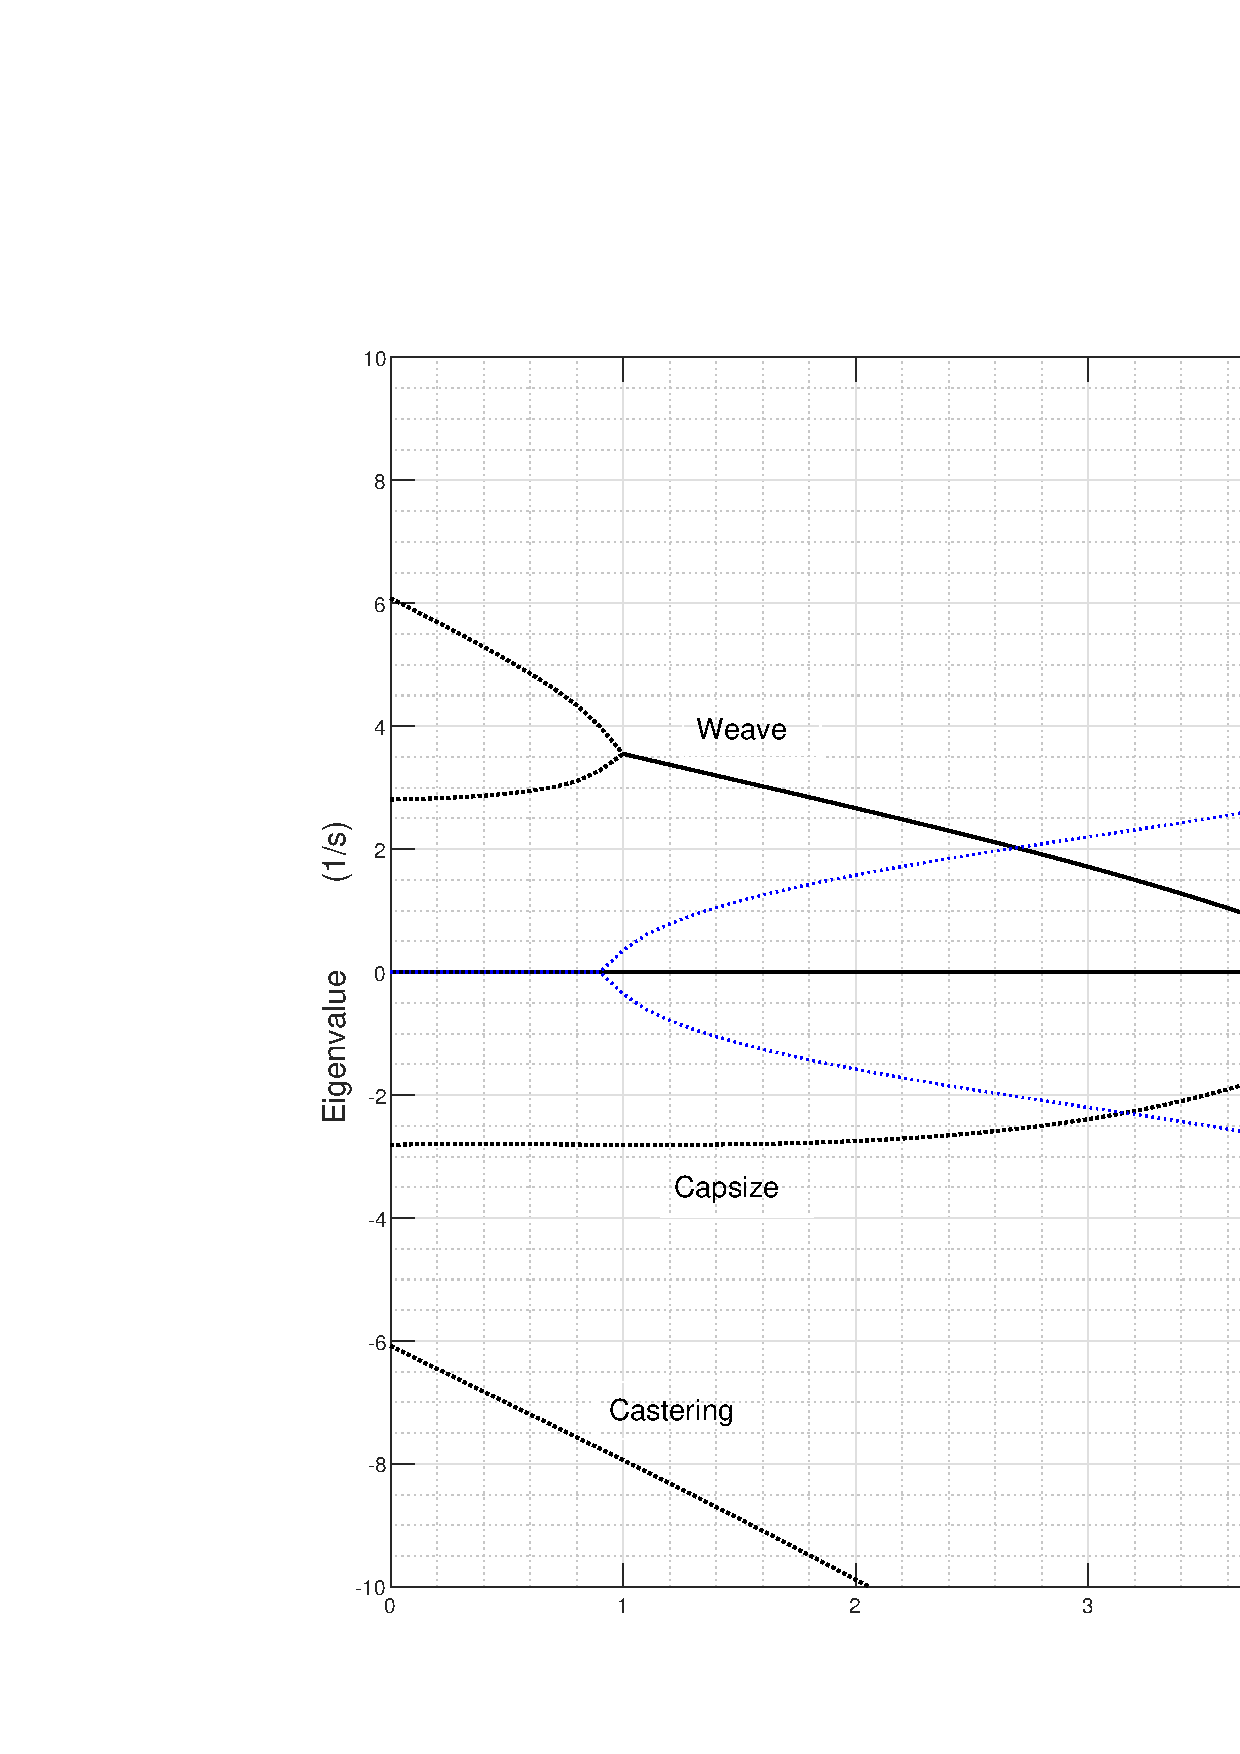
\includegraphics[scale=0.6]{images/root_locus_steerbywire.png}
    \caption{Root locus plot of the steer by wire bicycle. Dotted blue lines indicate the real part of the eigenvalues while dotted cyan show the imaginary part. The stable region corresponds to speeds  \ensuremath{4.39\lessapprox v \lessapprox 6.67\; \si{\meter\per\second}}}
    \label{fig:paper2}
\end{figure}
Since in the experimental setup the task could not be isolated to purely balance the equations are extended to include heading. Heading is defined as a linear combination of steer angle and steer rate as expressed by \citet{meijaard2007linearized} in \cref{eq:paper3}. 

\begin{equation}
    \dot{\psi}=\frac{v \delta+c \dot{\delta}}{w} \cos \lambda
    \label{eq:paper3}
    \end{equation}

When modeling the haptics off case of the steer-by-wire bicycle the dynamics of the plant need to change accordingly. In that configuration, the forcing steering input is directly proportional to steering acceleration, for this reason the second of the set of equations in \ref{eq:paper1} becomes :
\begin{align}
    M_{22}\ddot{\delta}+ M_{21}\ddot{\phi} + v{C_1}_{22}\dot{\delta} + v{C_1}_{21}\dot{\phi}+[g{K_0}_{22}+v^2{K_0}_{22}]\delta +[g{K_0}_{21}+v^2{K_0}_{21}]\delta &= T_{\delta} \\
    M_{22}\ddot{\delta} &= T_{\delta} \\
    I_{F_{xx}}\ddot{\delta} &= T_{\delta} 
\end{align}
where \ensuremath{I_{F_{xx}}} is the moment of inertia of the  decoupled handlebar assembly.
 
For control purposes \cref{eq:paper1} is expressed in state space form with state vector \ensuremath{\mathbf{x}=[\dot{\phi}, \dot{\delta}, \phi, \delta, \psi]^{T}}, forcing input \ensuremath{\mathbf{f}=T_{\delta}} and output equal to the full state. The  bike is assumed to be controlled only by a steering torque because according to both \citet{moore2012human} and \citet{weir1973manual}  the rear frame roll angle is mainly
 controlled by steering. 
 \begin{equation}
    \dot{\mathbf{x}}=\mathbf{A} \mathbf{x}+\mathbf{B} T_\delta + \mathbf{H}_d w
    \label{eq:bikeEOM}
\end{equation}
\begin{equation}
    \mathbf{y}=\mathbf{C} \mathbf{x}+\mathbf{D} T_\delta
\end{equation}
where matrices \ensuremath{A,B,C,D,H_d} are defined by:
\begin{align}
    \mathbf{A} &=\begin{bmatrix}
        -\mathbf{M}^{-1}v\mathbf{C}_{1} & -\mathbf{M}^{-1}(g \mathbf{K}_{0}+v^{2}\mathbf{K}_{2}) \\
        {\mathbf{I}_2}                    & {\mathbf{0}} \\  {\begin{matrix} {0} & { \frac{c\cdot cos\lambda}{w}}\end{matrix}} &  {\begin{matrix} 0 & { \frac{v \cdot cos\lambda}{w}}\end{matrix} } 
    \end{bmatrix} , \mathbf{B}=\left[ \begin{array}{c}{\mathbf{M}^{-1}} \\ {\mathbf{0}}\end{array}\right] \\
    \mathbf{C} &= {\mathbf{I}_5} , \mathbf{D}=\mathbf{0} \\
    \mathbf{H}_d &= \left[ \begin{array}{c}{\mathbf{M}^{-1}}{\begin{bmatrix} l_g \\ c_s\end{bmatrix} }  \\ {\mathbf{0}}\end{array}\right] 
\end{align}

\ensuremath{\mathbf{H}_d} is the matrix defining the dynamics of the lateral disturbance \ensuremath{w}. In this case the force application point was \ensuremath{l_g} distance from the ground. The constant \ensuremath{c_s} coefficient is due to the coupled roll to steer dynamics and is selected as a fraction of \ensuremath{w} similar to \citet{schwab2013}. This results in an additional  torque perturbation \ensuremath{T\delta } in the handlebars.

\subsection{Rider Control Model}\label{subsec:rider_model}

 The complete high level overview of the model is shown in \cref{fig:paper3}. The output state of the bicycle is concatenated with the steering torque to produce the complete vector of sensory inflow. The measurements attributed to the vestibular, visual and proprioceptive system of the human body are delayed and fed into a prediction algorithm that uses an internal model of the process dynamics to forward the measurements in time. This is made possible by the use of the efference copy, which is an internal copy of an outflowing, movement-producing signal generated by the motor system. The controller  is just a pure gain block with free parameters to be estimated through gray box system identification. The final control forcing input is produced after passing through a transfer function simulating the neuromuscular dynamics.
\begin{figure}[ht]
    \centering
    \captionsetup{justification=centering,margin=2cm}

    \includegraphics[scale=0.8]{images/high_level_block.pdf}
    \caption{Block diagram of the complete rider-bicycle model.} 
    \label{fig:paper3}
\end{figure}

The neuromuscular dynamics block works as a second order filter to simulate the limitations of the human response. In state space form this block is expressed by :

\begin{align}
\dot{x}_{nm} &= \begin{bmatrix}0 & 1 \\ -\omega^2 & -2\zeta\omega\end{bmatrix} \begin{bmatrix} T_\delta \\ \dot{T}_\delta\end{bmatrix} + \begin{bmatrix} 0 \\ \omega^2\end{bmatrix} a     \label{eq:gnmBLOCKA}    
    \\
y_{nm} &= \begin{bmatrix}1 & 0\end{bmatrix} \begin{bmatrix} T_\delta \\ \dot{T}_\delta\end{bmatrix}
    \label{eq:gnmBLOCKB}
\end{align}

where \ensuremath{\alpha} is the controller output representing the efferent neural signal, \ensuremath{\zeta} is the damping coefficient and \ensuremath{\omega_c} is the cutoff frequency. The latter two   parameters are chosen according to activation dynamics present in the shoulder joint \cite{happee2008posture}.

The steer angle \(\delta\) and steer rate \(\dot{\delta}\) feedback is attributed to the muscle spindles, while the torque feedback is made possible with the help of the golgi tendon organs. The roll and heading angle come from the visual system. Lastly the roll rate feedback is attributed to the vestibular system. 

The bicycle model of \cref{eq:bikeEOM} is combined with the neuromuscular dynamics block of \cref{eq:gnmBLOCKA,eq:gnmBLOCKB} to create a combined  plant with state \ensuremath{x=[\dot{\phi}, \dot{\delta}, \phi, \delta, \psi, T_\delta \dot{T}_\delta]^{T}} ,input \ensuremath{a} and \ensuremath{w} and output \ensuremath{y=[\dot{\phi}, \dot{\delta}, \phi, \delta, \psi, T_\delta]^{T}}. In order to make possible the implementation of the predictor which is discrete in nature the state space representation of the combined plant is discretized by zero order hold with a time step of 0.001 \si{\second}. The equivalent model block diagram is shown in \cref{fig:paper4}.

\subsubsection{The reafferent optimal predictor}
Many strategies to counter time delays have been proposed in literature. The most basic predictor is the Smith predictor, which has been explored in motor control research by \citet{miall1993cerebellum}. The Smith predictor compensates for time delays through the use of an internal forward model of the controlled dynamics and an internal model of the sensory delay pathways. The forward model works by utilizing an efferent signal of the control input while the comparison between prediction and measurement is trying to simulate the human's ability to distinguish between reafference and exafference.  Unfortunately the  most basic Smith predictor scheme does not work for unstable open loop systems \cite{smith1957closed}. In this work a modification to the normal Smith predictor scheme is suggested. In place of the forward model a discrete optimal predictor (tapped delay line) is used that forward simulates the amount of steps according to the model of sensory delay (see \cref{fig:delay_line}). This works like a resetting forward model that is updated every time step by the delayed state so the predictor loop does not become unstable. A tapped delay line without the Smith  correction can still work and has been implemented by \citet{van2001adaptive} for modeling stance control but it leads to predictions that do not contain any amount of the effect of the disturbance on the state. The block diagram of the predictor can be seen in \cref{fig:paper4}.

\begin{figure}[h!]
    \centering
    % \captionsetup{justification=centering,margin=2cm}

    \includegraphics[width=0.6\linewidth]{images/smith.pdf}
    \caption{Block diagram of the basic Smith Predictor scheme. The Smith Predictor uses an internal  forward model  to predict the delay-free response \ensuremath{\hat{y}} of the process. It then compares this prediction  with the desired setpoint \ensuremath{r} to decide what adjustments are needed (control \ensuremath{u}). To prevent drifting and reject external disturbances, the Smith predictor also compares the actual process output with a prediction \ensuremath{\hat{y}_d} that takes the dead time into account. The gap \ensuremath{y_e=y_d-\hat{y}_d} is fed back  and contributes to the overall controller input. Note that \ensuremath{y_e} amounts to the perceived state mismatch delayed by the duration of dead time.}
    \label{fig:smith}
\end{figure}


\begin{figure}[h!]
    \centering
    % \captionsetup{justification=centering,margin=2cm}

    \includegraphics[width=\linewidth,trim={0 4.2cm 0 2cm},clip]{images/predictor_plots/tapped_delay.pdf}
    \caption{The discrete optimal predictor consists of a tapped delay line. The tapped delay line used in this work is a forward simulation of the discretised dynamics of the bicycle including neuromuscular dynamics. It uses the efference copy of the known previous control input \ensuremath{a_n}  and the delayed estimate \ensuremath{y^d_n}. \ensuremath{A^*_m} and \ensuremath{B^*_m} are the best available discrete approximation of these dynamics.}
    \label{fig:delay_line}
\end{figure}


 \begin{figure}[ht]
    \centering
    % \captionsetup{justification=centering,margin=2cm}

    \includegraphics[width=\linewidth,trim={0 2.8cm 0 2cm},clip]{images/low_level_block.pdf}
    \caption{Block diagram of the Reafferent Optimal Prediction Model. \ensuremath{A^*} ,\ensuremath{B^*}, \ensuremath{H_d^*} are the discretized matrices of the combined plant dynamics. Matrices \ensuremath{A_m^*} ,\ensuremath{B_m^*} express the dynamics of the internal model of the process. When the internal model is assumed to be perfect \ensuremath{A_m^*=A^*} and \ensuremath{B^*=B^*}. The delayed output measurement is forwarded in time (d times) in the tapped delay line to produce the first undelayed estimate of the output \ensuremath{\hat{y}^p}, which is again delayed through a model of the  internal time delay. The difference between this re-delayed prediction with the delayed measurements creates the error \ensuremath{e} which is added back to  \ensuremath{\hat{y}^p}  to create the final corrected prediction \ensuremath{\hat{y}^c}. }
    \label{fig:paper4}
\end{figure}

\subsection{Parameter Estimation }

In order to assess the effectiveness of the torque feedback loop, three models of incremental complexity are used. In the first the feedback pathways are fed into the controller without delays. In the second delays are added. The third one compensates for time delays by the use of the Reafferent Optimal Predictor (ROP). The three models have the  controller gains as free parameters. More specifically, the gains are estimated by fitting the model output into the non-parametric data-set derived in \cite{dialynaseffect}.  The gains were estimated by minimization of the cost function 
\begin{equation}
    V_{N}(\boldsymbol{\theta})=\frac{1}{N} \mathlarger{\mathlarger{\mathlarger{\sum}}}_{k=1}^{N}\left[64\frac{\left(\hat{y}^{\delta}_k(\mathbf{\theta})-y^\delta_k\right)^{2}}{\underset{k}{\max} \left(y^\delta_k\right)^2}+11\frac{\left(\hat{y}^{\psi}_k(\mathbf{\theta})-y^\psi_k\right)^{2}}{\underset{k}{\max} \left(y^\psi_k\right)^2}+7\cdot10^{-6}\frac{\left(\hat{y}^{T_\delta}_k(\mathbf{\theta})\right)^2}{\underset{k}{\max} \left(y^{T_\delta}_k\right)^2}\right]
    \label{eq:cost}
    \end{equation}

where \ensuremath{\boldsymbol{\theta}} is a vector containing all the free parameters, \ensuremath{\hat{y}^{\delta}} and \ensuremath{\hat{y}^{\psi}} are the outputs of the simulation for the measured external disturbance \ensuremath{w} and the vector of parameters  \ensuremath{\boldsymbol{\theta}} for steer angle \ensuremath{\delta} and heading angle \ensuremath{\psi}  respectively, while \ensuremath{y^\delta} and \ensuremath{y^\psi} are the outputs of the non-parametric model.

The first two terms  of the cost function are trying to match the steering and heading  response of the parametric model with that one of the non-parametric model, while the third on minimizes the amount of input torque generated in order to produce the best possible fit while maintaining minimal control effort. The weights are chosen heuristically. For optimization the genetic algorithm with a fitness limit of 0.03 is first  used in order to produce a good starting parameter vector for gradient descend algorithm to take over, which finally finds the closest possible estimate of the global minimum. For the genetic algorithm a crossover fraction of 0.85  along with a population size 10 times the length of the parameter vector is used.

The gains attributed to the muscle spindle sensors (\ensuremath{K_\delta} and \ensuremath{K_{\dot{\delta}}}) are constrained to be only positive. The assumption is that they work like a delayed steering stiffness and damping. Additionally, the gains \ensuremath{K_\psi} and \ensuremath{K_\phi}  are constrained to fall under -250 and 250 \si{\kilogram\square\meter\per\second}.  When left unconstrained these parameters drive the whole gain vector to unrealistic values for insignificant amount of fitting performance increase (\ensuremath{<0.1\%}).

The impulse response function of the median rider is used. This is determined by taking the mean impulse response function of each measured output and finding the participant which had the highest variance accounted for between the individual response and the mean across all speed levels for all filtered outputs. Each system was identified for three different model conditions: 
\begin{enumerate}
    \item  6 feedback pathways including torque feedback
    \item  5 feedback pathways excluding torque feedback
    \item  6 feedback pathways including torque feedback but bicycle dynamics are switch to "haptics off".
\end{enumerate}
In the thrid condition the internal model used in the predictor is not updated to reflect the changed bicycle dyanamics. This assumption is made due to the fact that no adaptation time  was noted in the experiments for any of the participants when switching the steering configurations so significant tuning of an internal model is not realistic. 

 As metric of model validity the variance accounted for between parametric and non-parametric output is used, defined as
\begin{equation}
\mathrm{VAF_d}(\boldsymbol{\theta})=1 -\sum_{k=1}^{n}\left(y^{d}(k)-\hat{y}^{d}(k, \boldsymbol{\theta})\right)^{2} / \sum_{k=1}^{n}\left(y^{d}(k)^{2}\right)
\end{equation} 
where \ensuremath{d=\{\phi,\delta,\psi\}}. 

In order to assess the importance of the torque feedback, the uncertainty of each parameter is found. Parameters with the lowest uncertainty contribute more to the fit so they are deemed more important. To find the uncertainty the covariance matrix is estimated from :
\begin{align}
    \operatorname{cov}_{\hat{\theta}}  &=V_N(\boldsymbol{\hat{\theta}})\boldsymbol{H}(\boldsymbol{\hat{\theta}})^{-1}
    \label{fig:cov_mat}
    \\ \text{with} \;\;\;\;  \boldsymbol{H}(\boldsymbol{\hat{\theta}})&= \frac{\partial^{2} V_N}{\partial \theta_{i} \partial \theta_{j}}
\end{align}

where \ensuremath{\boldsymbol{\hat{\theta}}} is the closest estimate to the true parameter vector \ensuremath{\theta^*} that produces the true global minimum and \ensuremath{\boldsymbol{H}} is the hessian matrix numerically estimated by the gradient descend algorithm.  However, since bigger parameters are going to have naturally larger variances the diagonal values are normalized by the parameter value to produce the coefficient of variation.

\begin{equation}
    CV_{i}=\sqrt{\frac{\sigma^{2}_{\hat{\theta_i}}}{\hat{\theta}_i^2}}
    \end{equation}

    where \ensuremath{\sigma^{2}_{\hat{\theta_i}}} are the diagonal elements of \ensuremath{ \operatorname{cov}_{\hat{\theta}}}.
% As far as the delays are concerned for \ensuremath{\delta} and \ensuremath{\dot{\delta}} which are attributed to the muscle spindle sensors and for the torque feedback which is attributed to the golgi tendon organs  a delay of 25 \si{\milli\second} is chosen \cite{van2002identification,de2002adaptation}. For the feedback states attributed to visual feedback such as the roll angle \ensuremath{\phi} and yaw angle \ensuremath{\psi} a much greater delay of 200 \si{\milli\second} is chosen. Finally for  the vestibular roll rate feedback a delay of 50 \si{\milli\second} is implemented \cite{barnett2013vestibular}. 
% \cite{whipple1899stability}


\section{Results}


\subsection{Zero Delay Model}
The results of the zero delay model for the median rider are presented in \cref{tb:no_delay}. A \ensuremath{\mathit{VAF}} of over 90 \% is easily achieved for both steer angle and heading, while for roll the discrepancy is larger. A  look into how the model approximates the measured rider input and bicycle states for all forward speeds is seen in \cref{fig:zdm_fitA,fig:zdm_fitB}. Even in the ideal case with zero delays, the model inputs seems to lag behind the measured applied rider torque.

% \begin{figure}[!h]
%     % \centering
%     % \captionsetup{justification=centering,margin=2cm}
%     \makebox[\textwidth][c]{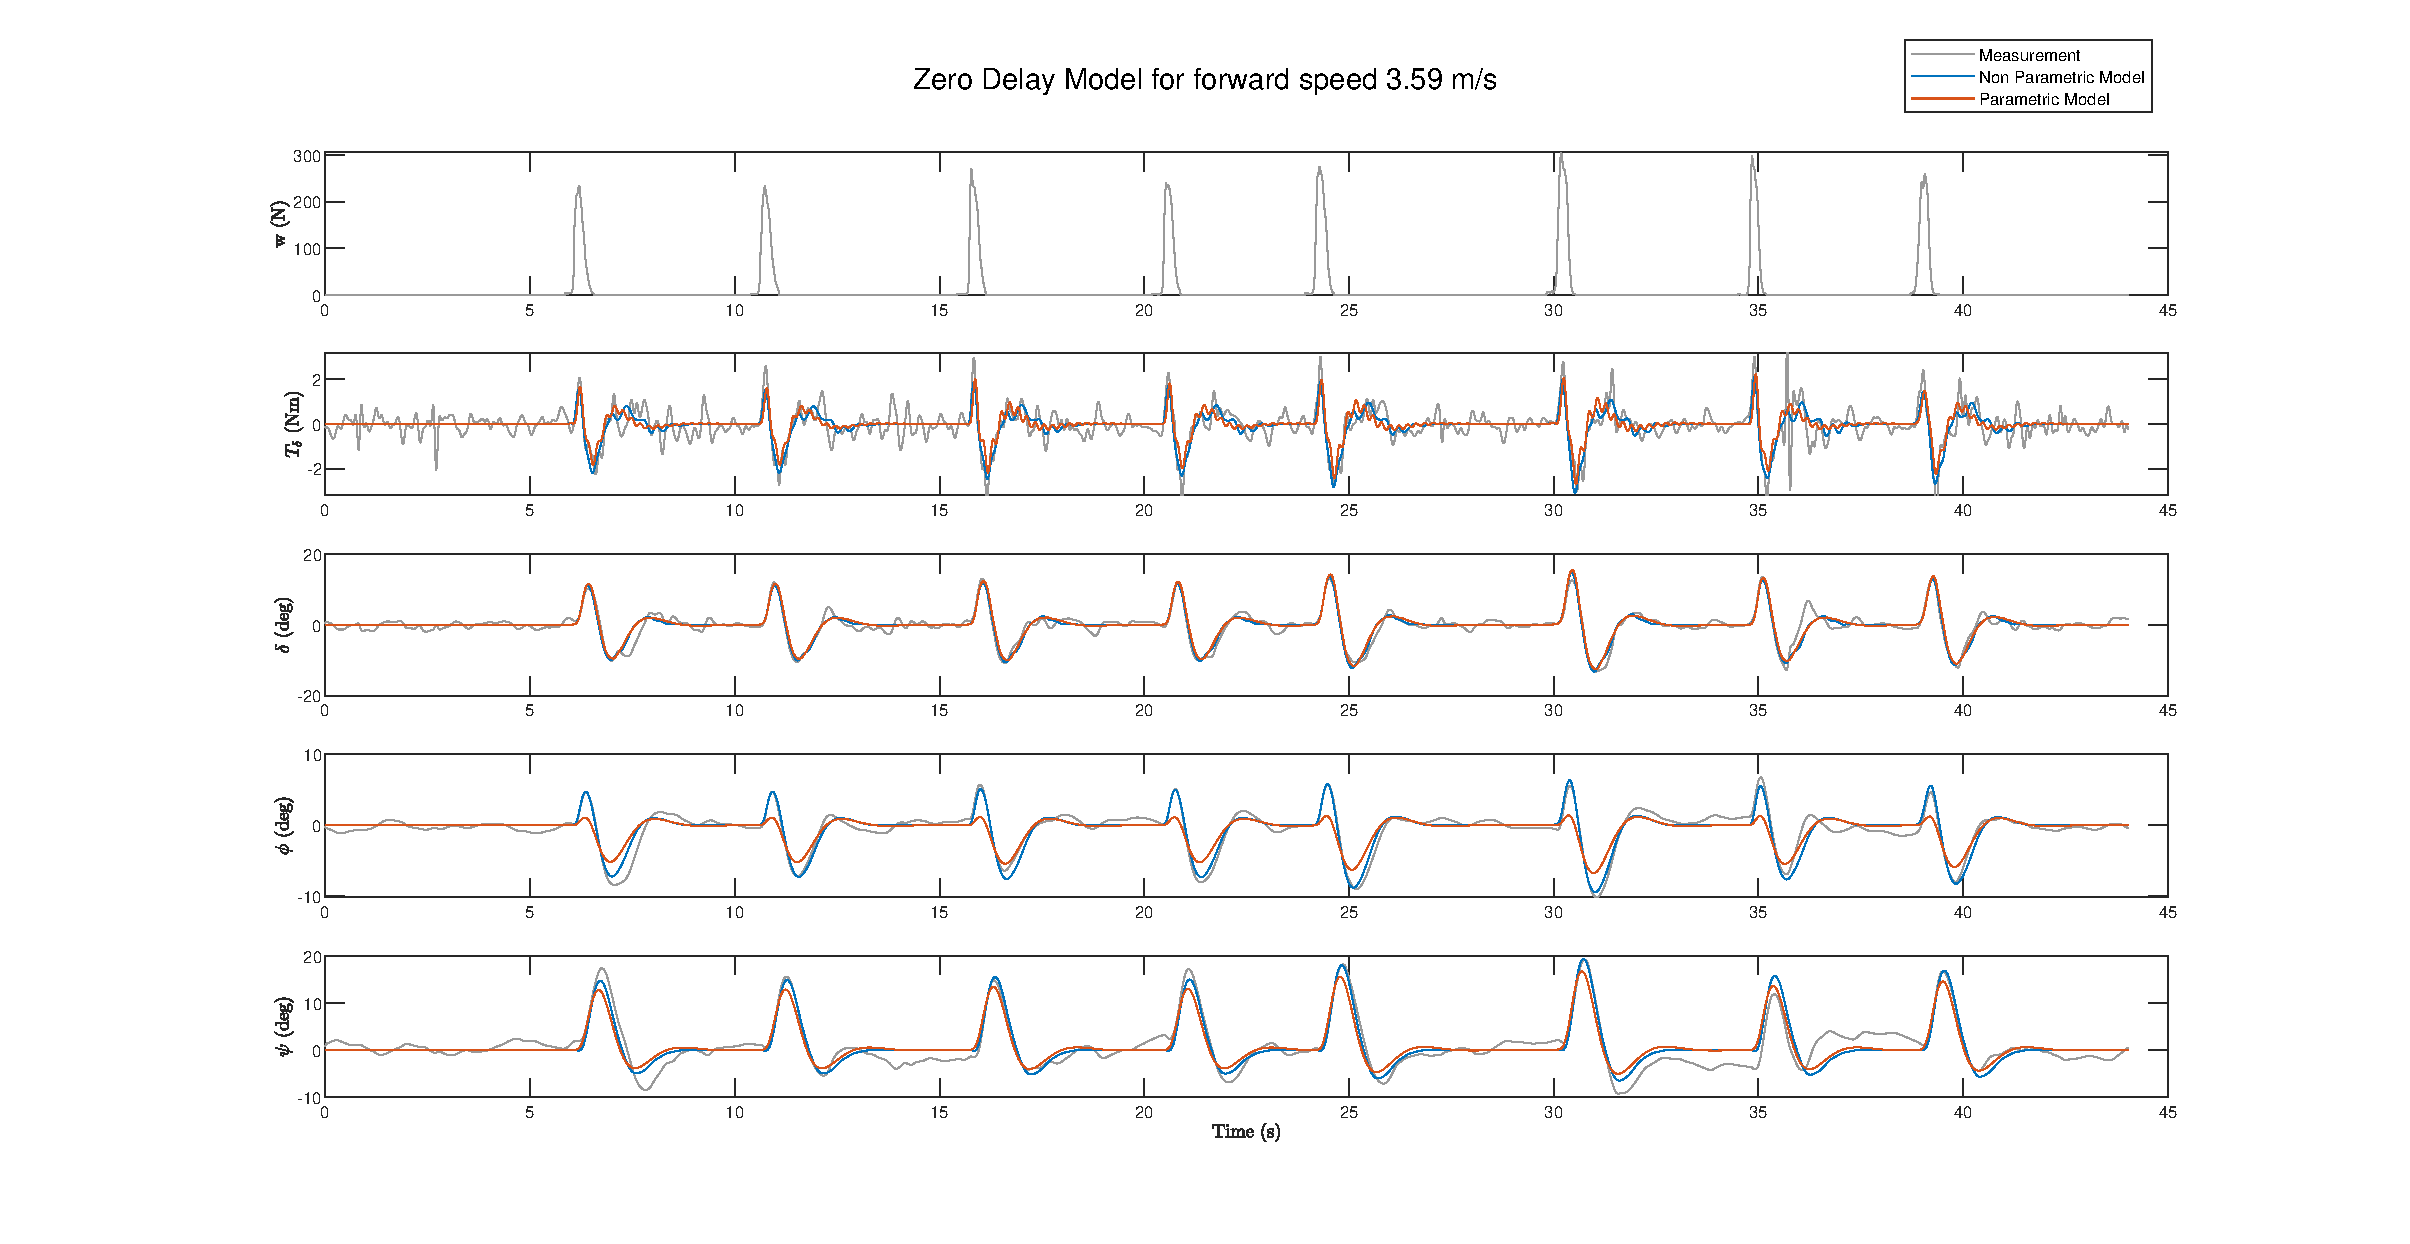
\includegraphics[width=1.4\textwidth]{images/no_delay_result1.eps}}
%     % 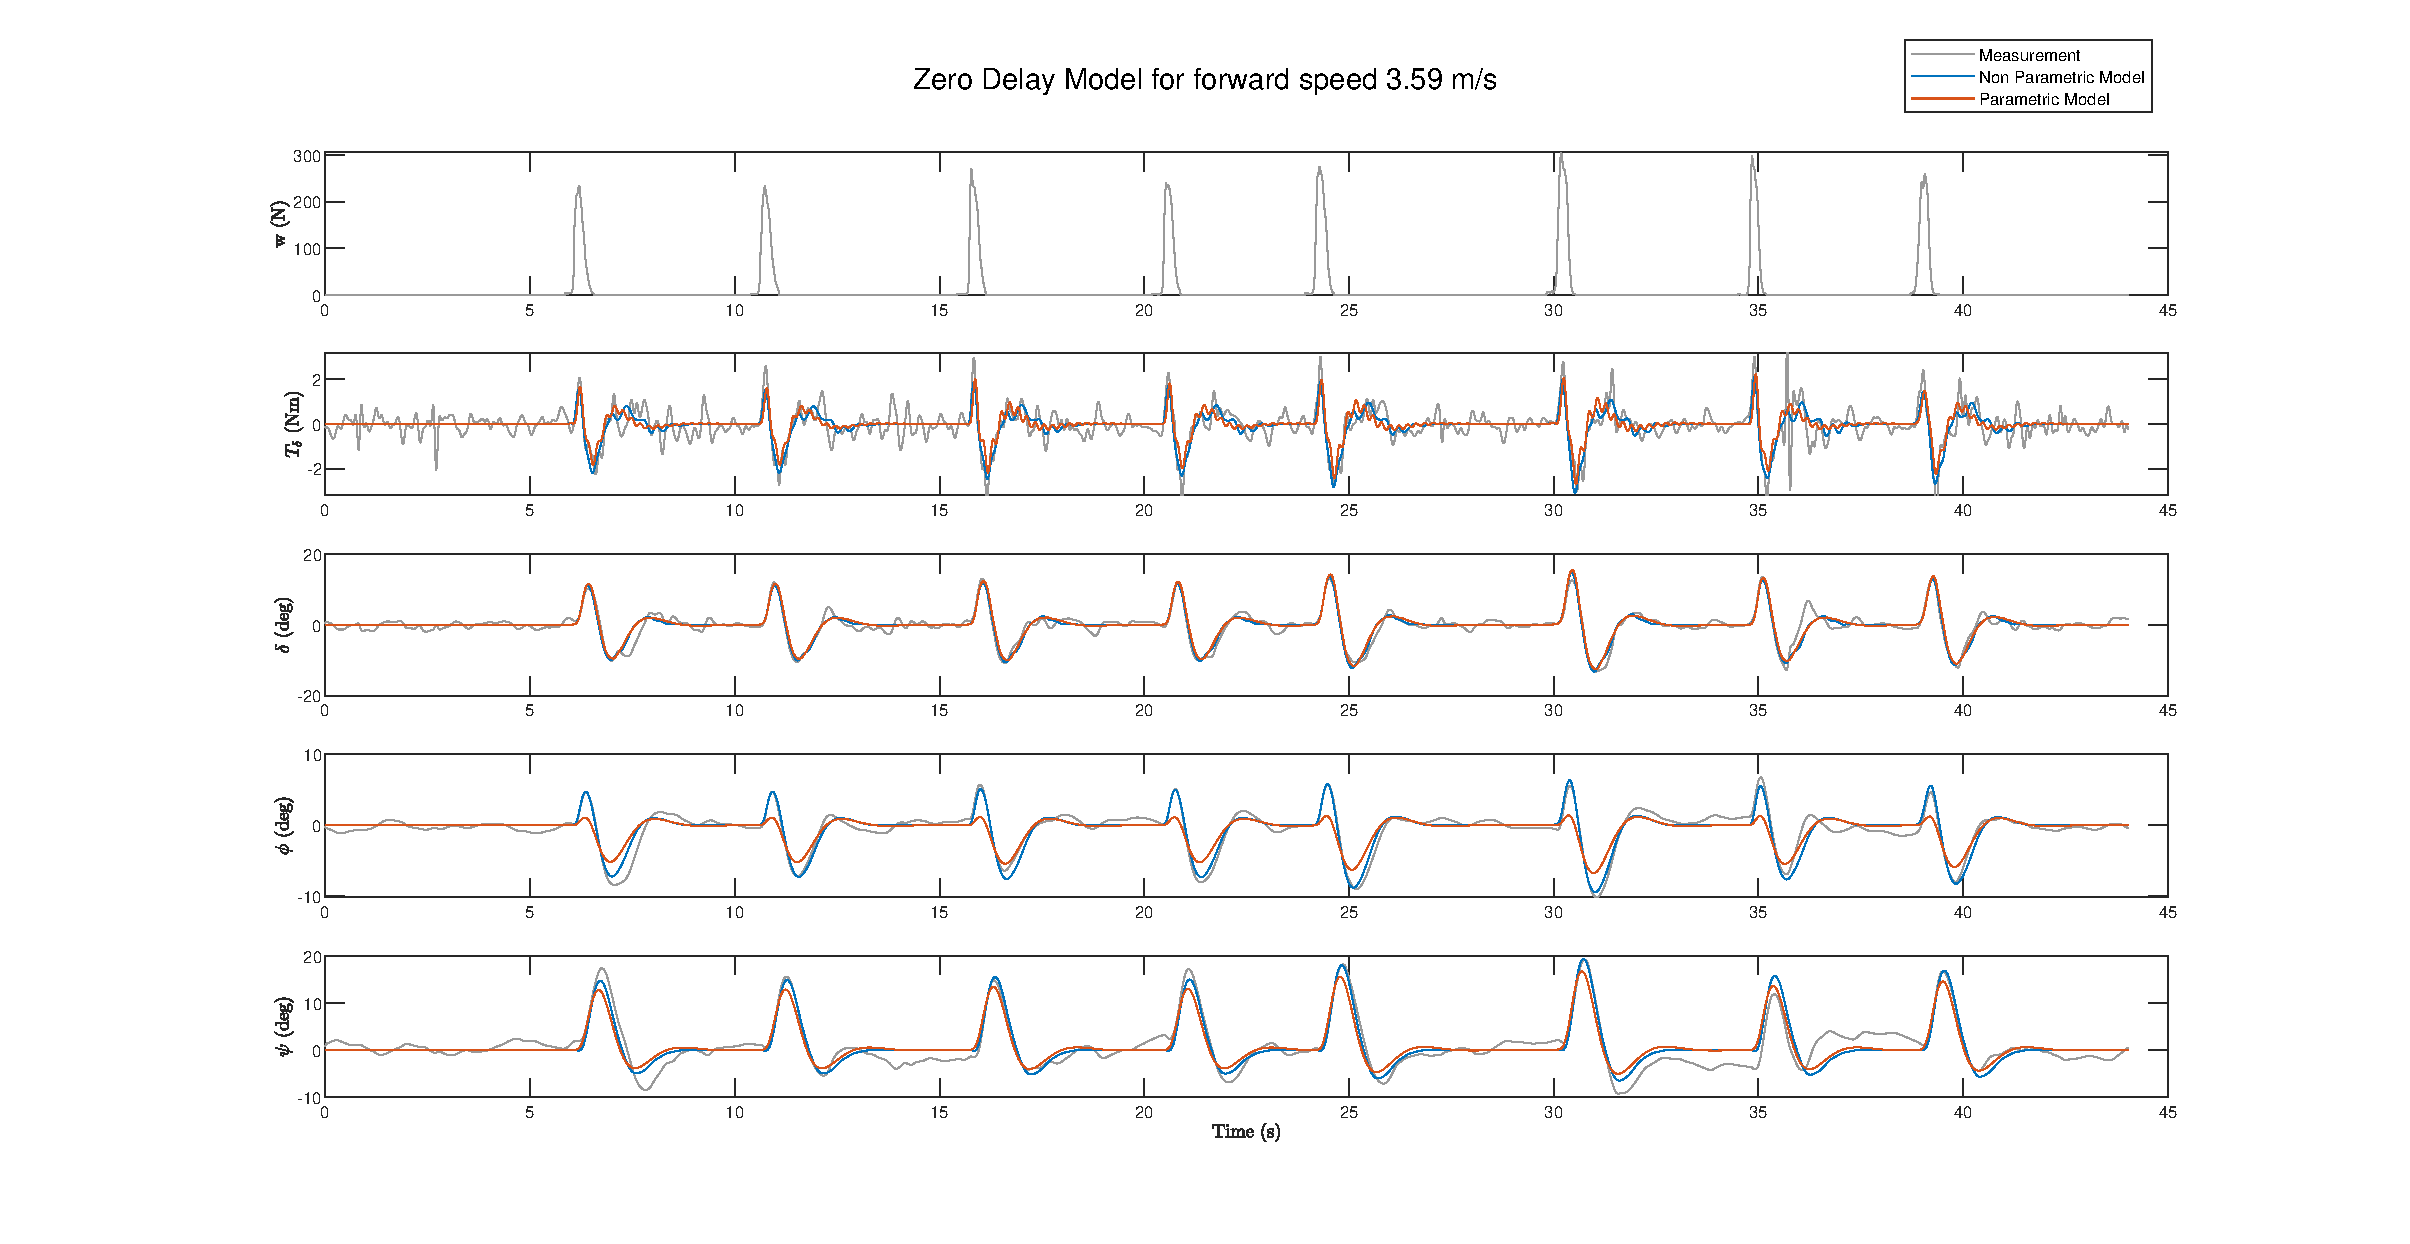
\includegraphics[width=\textwidth]{images/no_delay_result1.eps}
%     \caption{Comparison between parametric model output, non-parametric model ouput and measured signals for the speed level of 3.6 \si{\meter\per\second} for the case where torque feedback activated.}
%     \label{fig:paper5}
% \end{figure}

\begin{figure}[!h]
    \centering
    \begin{subfigure}[b]{\textwidth}
        \centering
        \makebox[\textwidth][c]{ 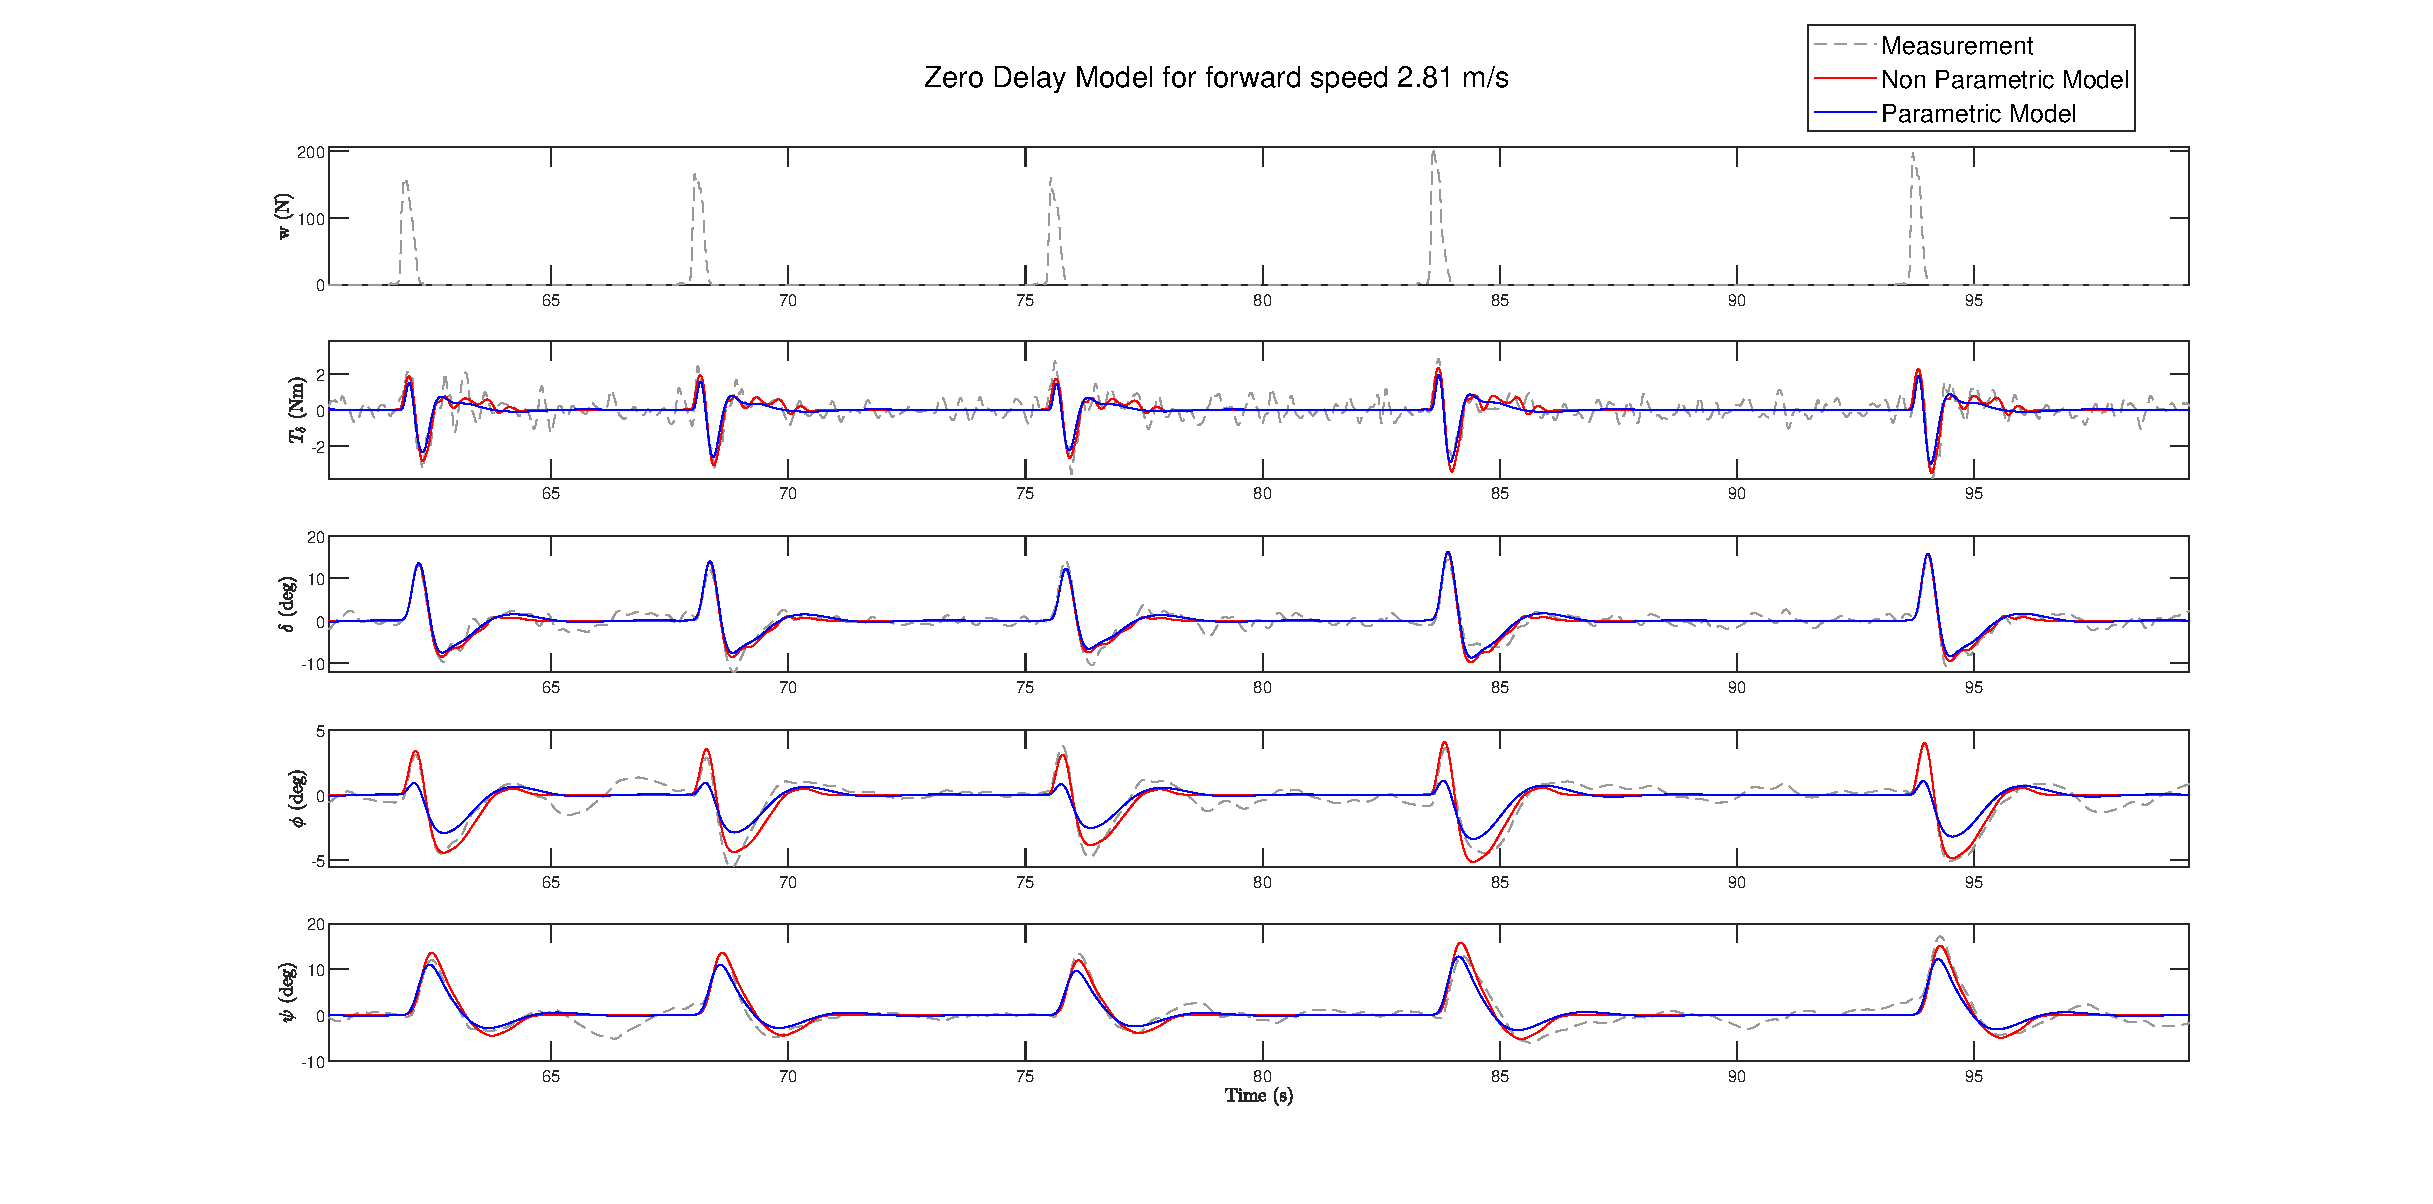
\includegraphics[width=1.4\textwidth]{images/raw_fit_plots/nodelay_28.eps}}
        \caption{}
        \label{fig:zdm_fit1}
    \end{subfigure}
    \begin{subfigure}[b]{\textwidth}
        \centering
        \makebox[\textwidth][c]{ \includegraphics[width=1.4\textwidth]{images/raw_fit_plots/nodelay_36.eps}}
        \caption{}
        \label{fig:zdm_fit2}
    \end{subfigure}
    
    \caption{Comparison between parametric model output (Zero Delay Model), non-parametric model output and measured signals for the two lowest speed levels for the case where torque feedback is present in the rider control model and bicycle is operating under the "haptics on" dynamics.}
    \label{fig:zdm_fitA}
 \end{figure}

 \begin{figure}
    \centering
    \begin{subfigure}[b]{\textwidth}
        \centering
        \makebox[\textwidth][c]{ \includegraphics[width=1.4\textwidth]{images/raw_fit_plots/nodelay_46.eps}}
        \caption{}
        \label{fig:zdm_fit3}
    \end{subfigure}
    \begin{subfigure}[b]{\textwidth}
        \centering
        \makebox[\textwidth][c]{ \includegraphics[width=1.4\textwidth]{images/raw_fit_plots/nodelay_57.eps}}
        \caption{}
        \label{fig:zdm_fit4}
    \end{subfigure}
    
    \caption{Comparison between parametric model output (Zero Delay Model), non-parametric model output and measured signals for the two highest speed levels for the case where torque feedback is present in the rider control model and bicycle is operating under the "haptics on" dynamics.}
    \label{fig:zdm_fitB}
 \end{figure}
From the coefficient of variation, no real difference between the levels of normalized uncertainty is noted. However, \ensuremath{\mathit{VAF}_\delta} drops more than 15-20\% when \ensuremath{T_\delta} feedback is turned off (see \cref{tb:no_delay}), which indicates significant impact on the fit. Additionally,  the steering angle and torque response   becomes significantly more oscillatory when \ensuremath{K_{T_\delta}} feedback is turned off (see \cref{fig:paper6}). Roll stabilization performance does not seem to be affected, however steering effort considerably does. Regarding the haptics off case, where the intent is to simulate the steering feel the participants experienced in the second experimental condition, the level of steering fit degradation is small (\ensuremath{<3\%}).

\begin{figure}[!h]
    \centering
    \captionsetup{justification=centering,margin=2cm}

    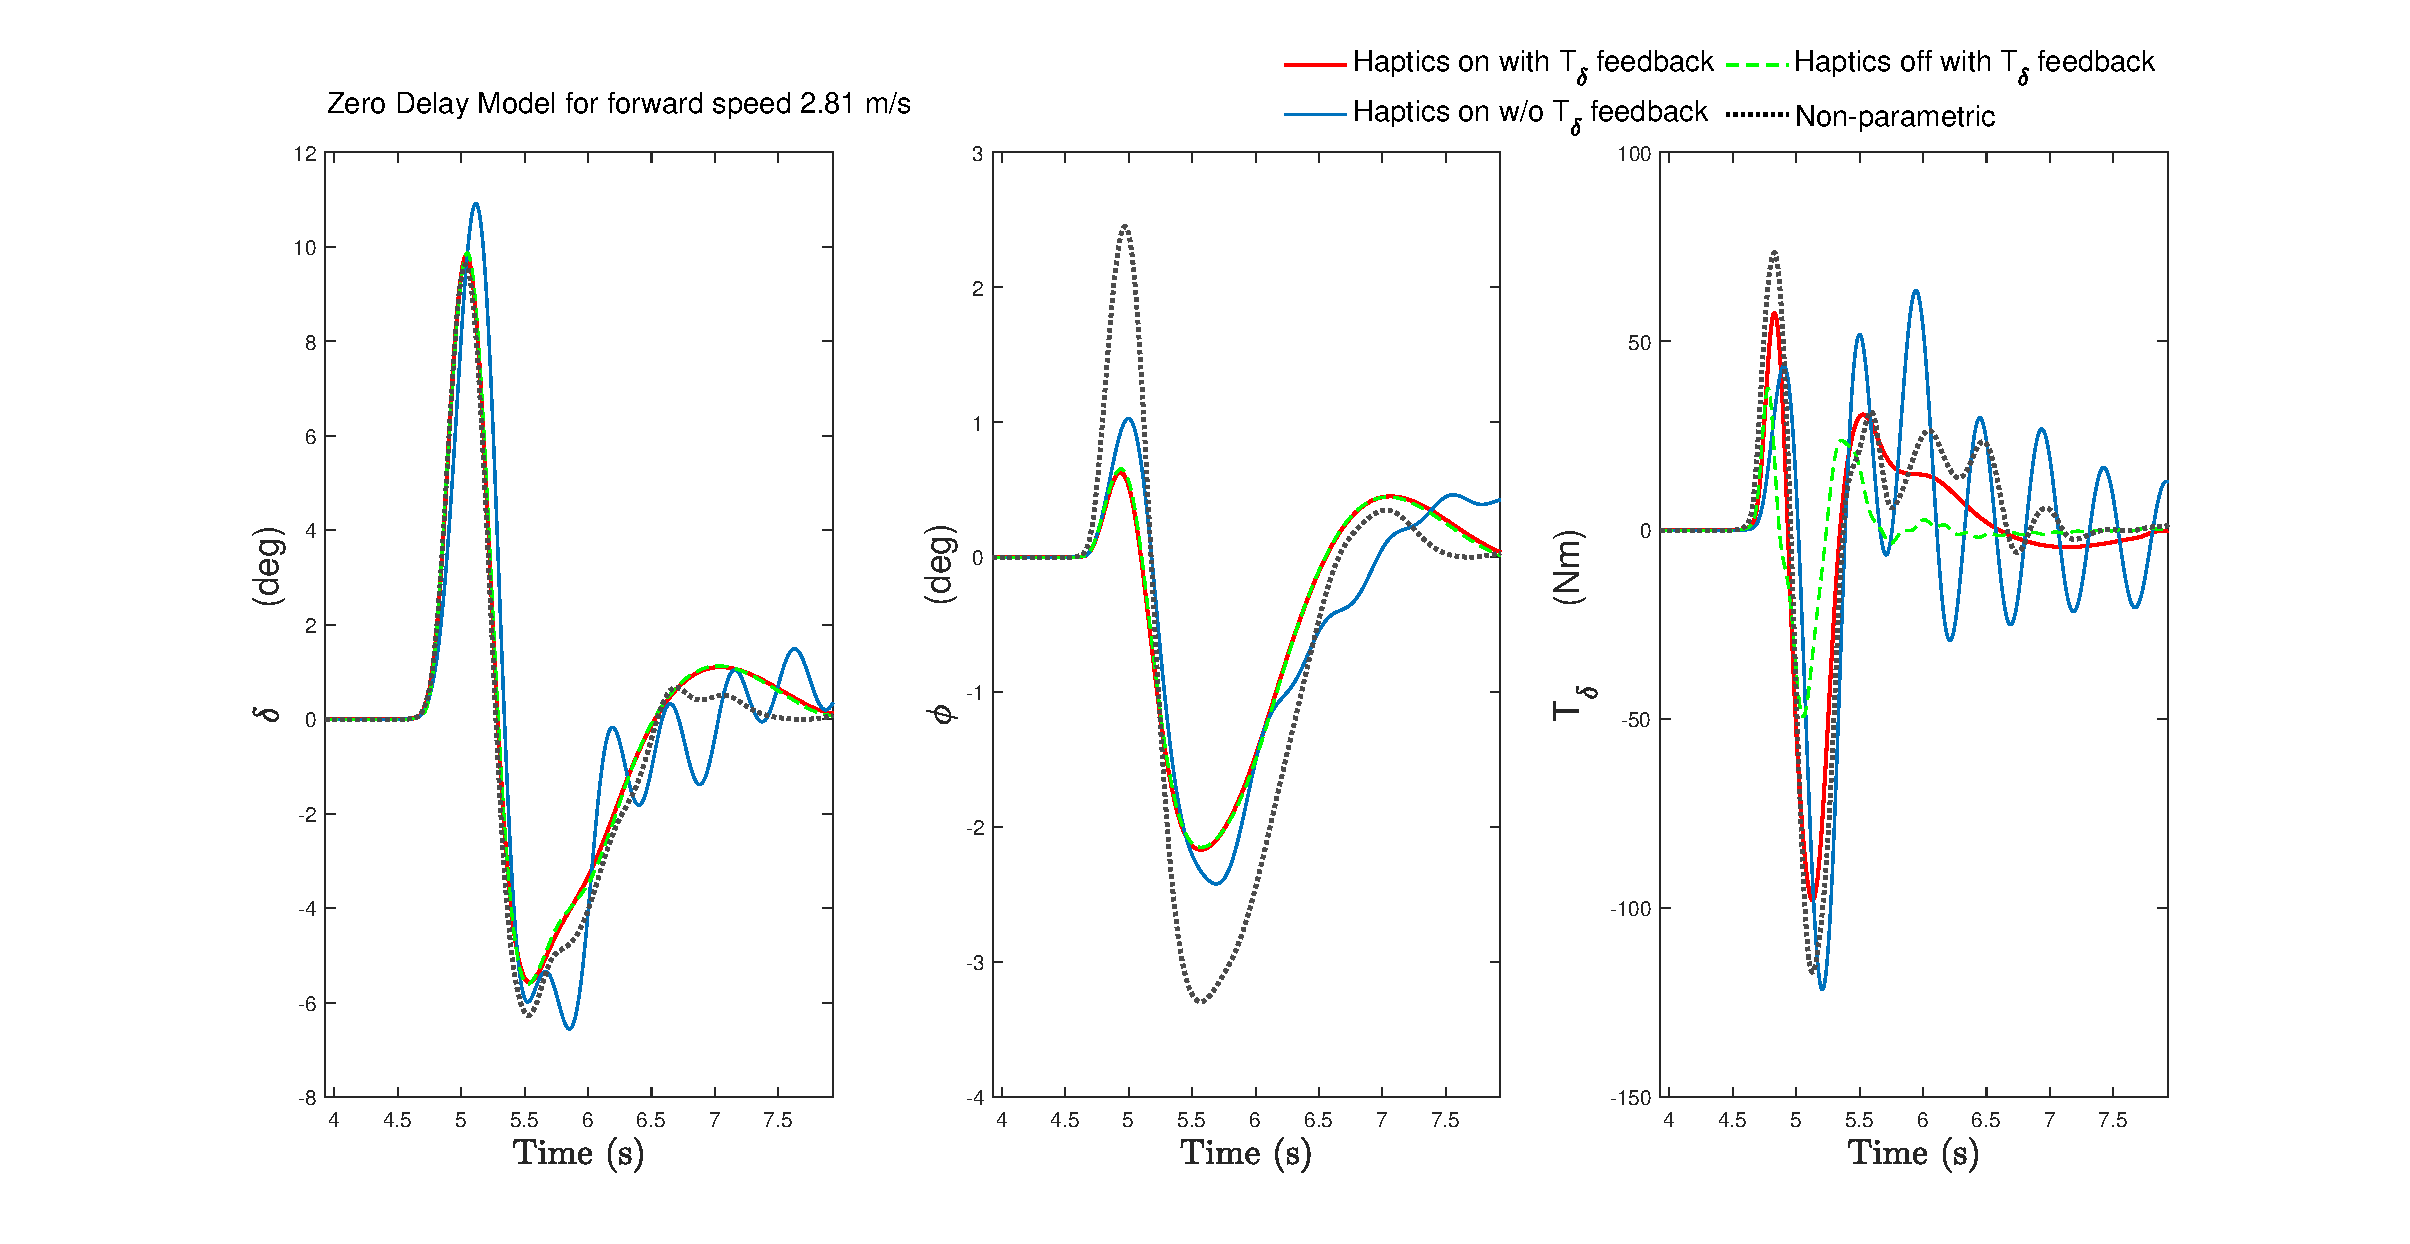
\includegraphics[width=\textwidth]{images/fb_compare_plots/no_delay_fb_compare28.eps}
    \caption{Steering, roll angles and input rider torque compared among torque feedback levels  for the forward speed of 2.81 \si{\meter\per\second} in the Zero Delay Model. Response of the first disturbance in the run is shown.}
    \label{fig:paper6}
\end{figure}



\subsection{Variable Delay Model}
The same procedure is repeated for the gray box model but now introducing  delays in all feedback pathways. For \ensuremath{\delta} and \ensuremath{\dot{\delta}} which are attributed to the muscle spindle sensors and for the torque feedback which is attributed to the golgi tendon organs  a delay of 25 \si{\milli\second} is chosen \cite{van2002identification,de2002adaptation}. For the feedback states attributed to visual feedback such as the roll angle \ensuremath{\phi} and yaw angle \ensuremath{\psi} a much greater delay of 200 \si{\milli\second} is chosen \cite{kawakami2002visual}. Finally for  the vestibular roll rate feedback a delay of 50 \si{\milli\second} is implemented \cite{barnett2013vestibular}. 

The results of the variable delay model for the median rider are presented in \cref{tb:variable}.  Despite the fact that significant delay is introduced into the system the torque feedback loop manages to compensate maintaining a \ensuremath{\mathit{VAF}_\delta} of over 90 \% for low speed levels (see \cref{tb:variable} and \cref{fig:dm_fitA}). In \cref{fig:dm_fitA,fig:dm_fitB} the delayed response of the simulated compared to the real rider is visible between the red and blue lines in the rider torque graph. This is further exaggerated in the two remaining conditions resulting in much more oscillatory steering responses with a visible impact on roll stabilization (see \cref{fig:paper8}). The coefficient of variation of the \ensuremath{K_\delta} parameter in the haptics on with \ensuremath{T_\delta} feedback connected is the highest especially for the two highest speed levels, which indicates that this parameter is not significant for the fit. Between \ensuremath{K_{T_\delta}} feedback on and feedback off, a much larger drop in VAF is noted. Additionally, contrary to the zero delay model an equally significant drop in the fit is noted for the haptics off case. 






\begin{figure}[!h]
    \centering
    \begin{subfigure}[b]{\textwidth}
        \centering
        \makebox[\textwidth][c]{ 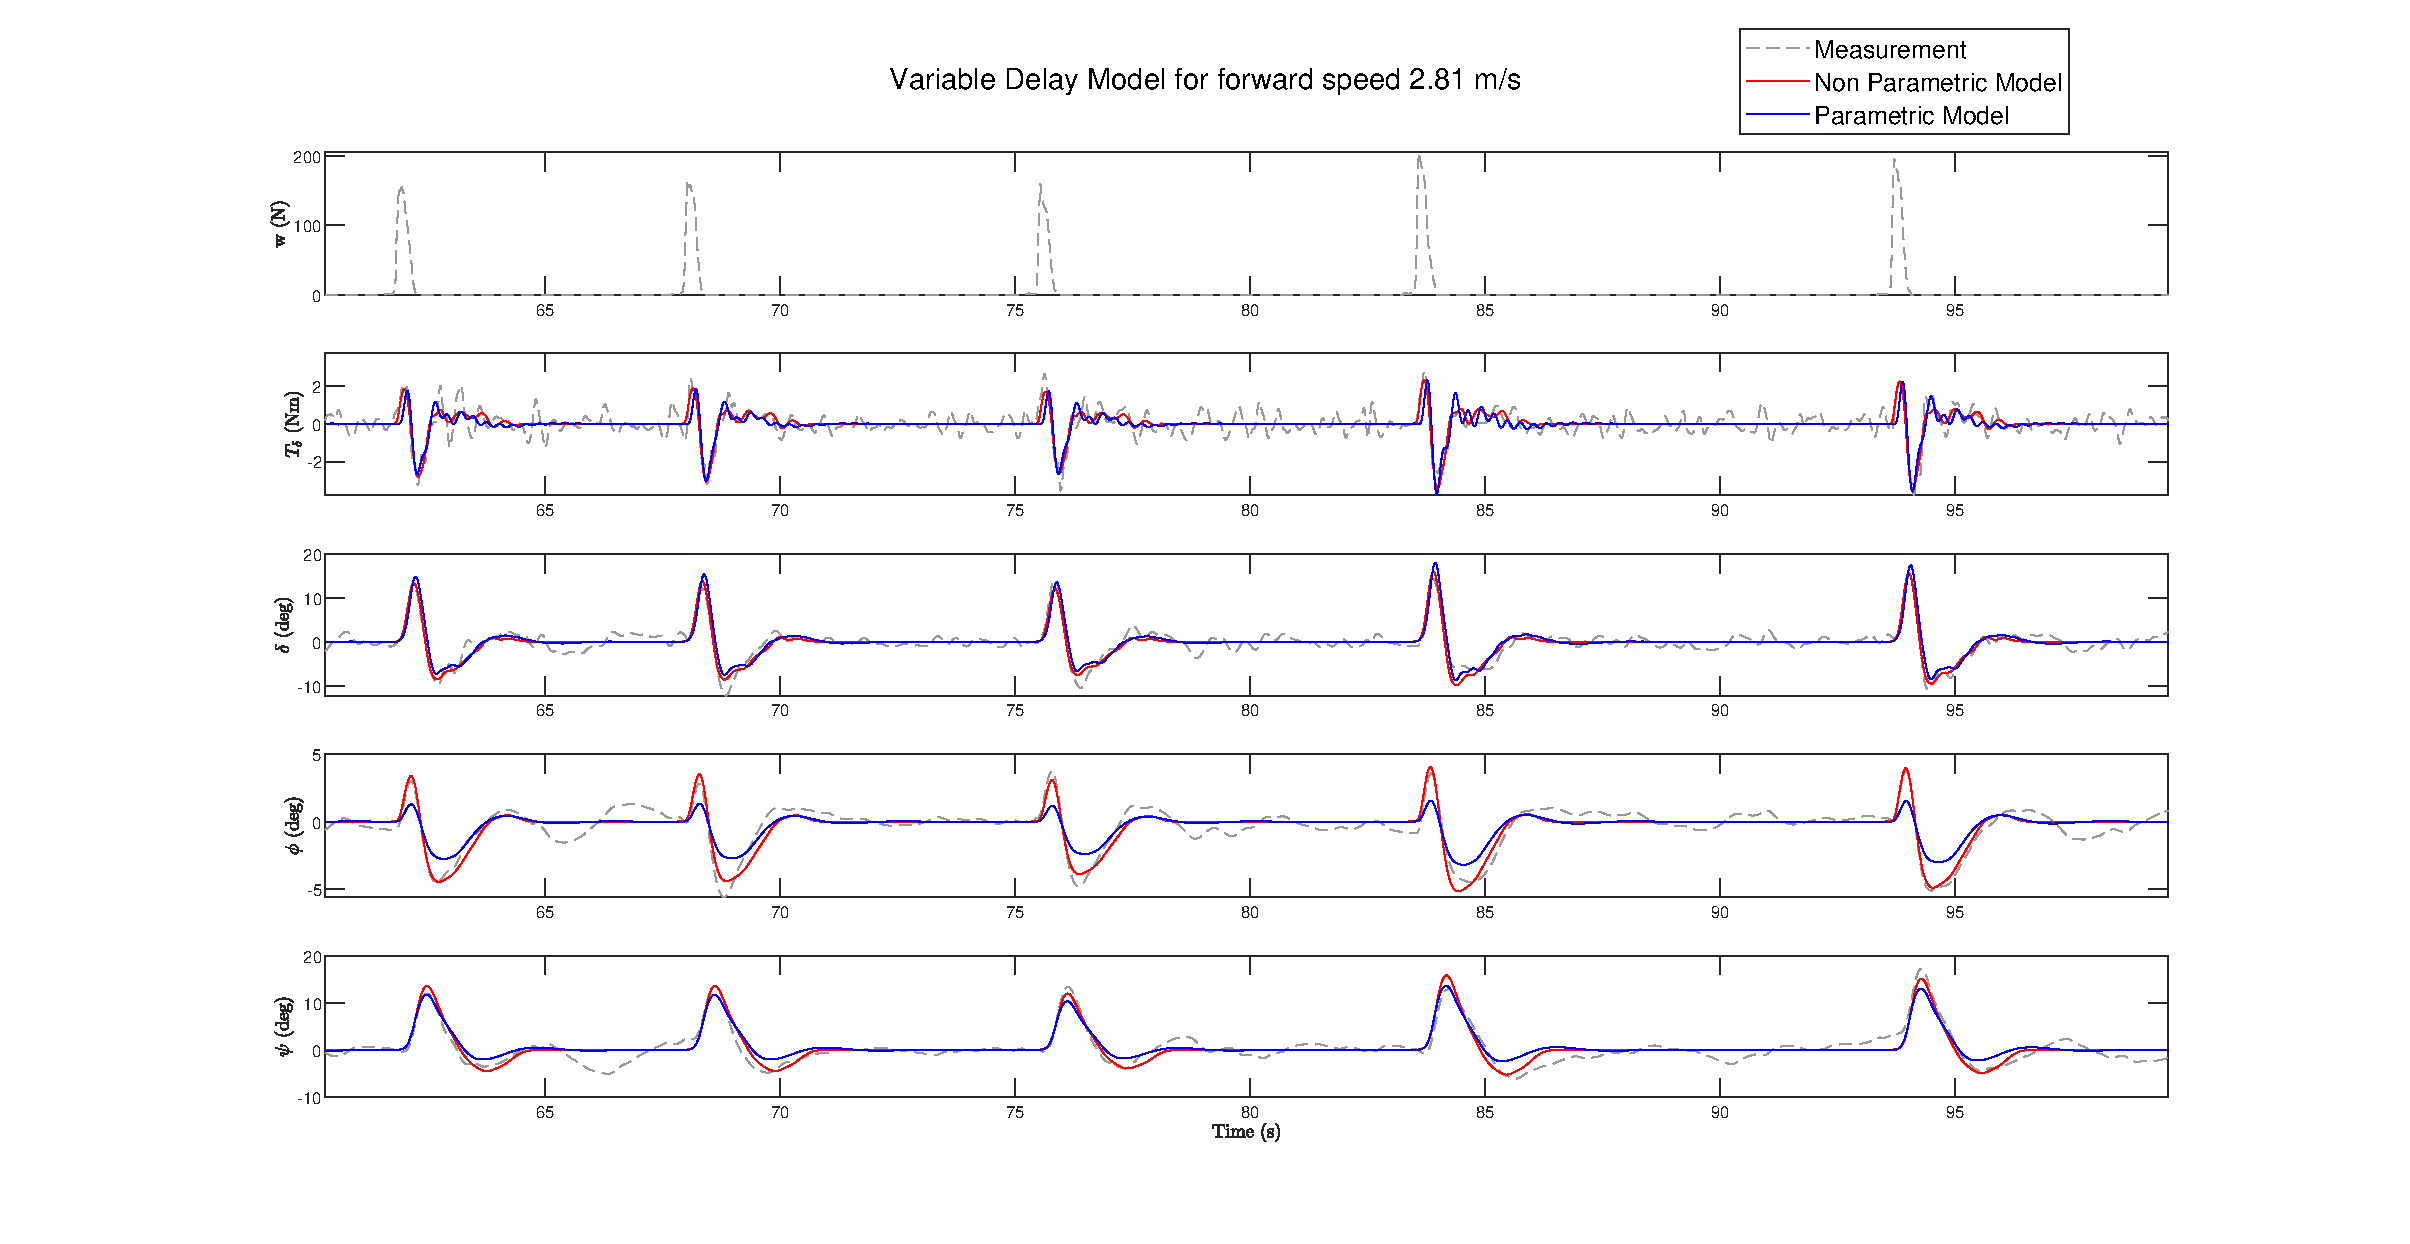
\includegraphics[width=1.4\textwidth]{images/raw_fit_plots/delay_28.eps}}
        \caption{}
        \label{fig:dm_fit1}
    \end{subfigure}
    \begin{subfigure}[b]{\textwidth}
        \centering
        \makebox[\textwidth][c]{ 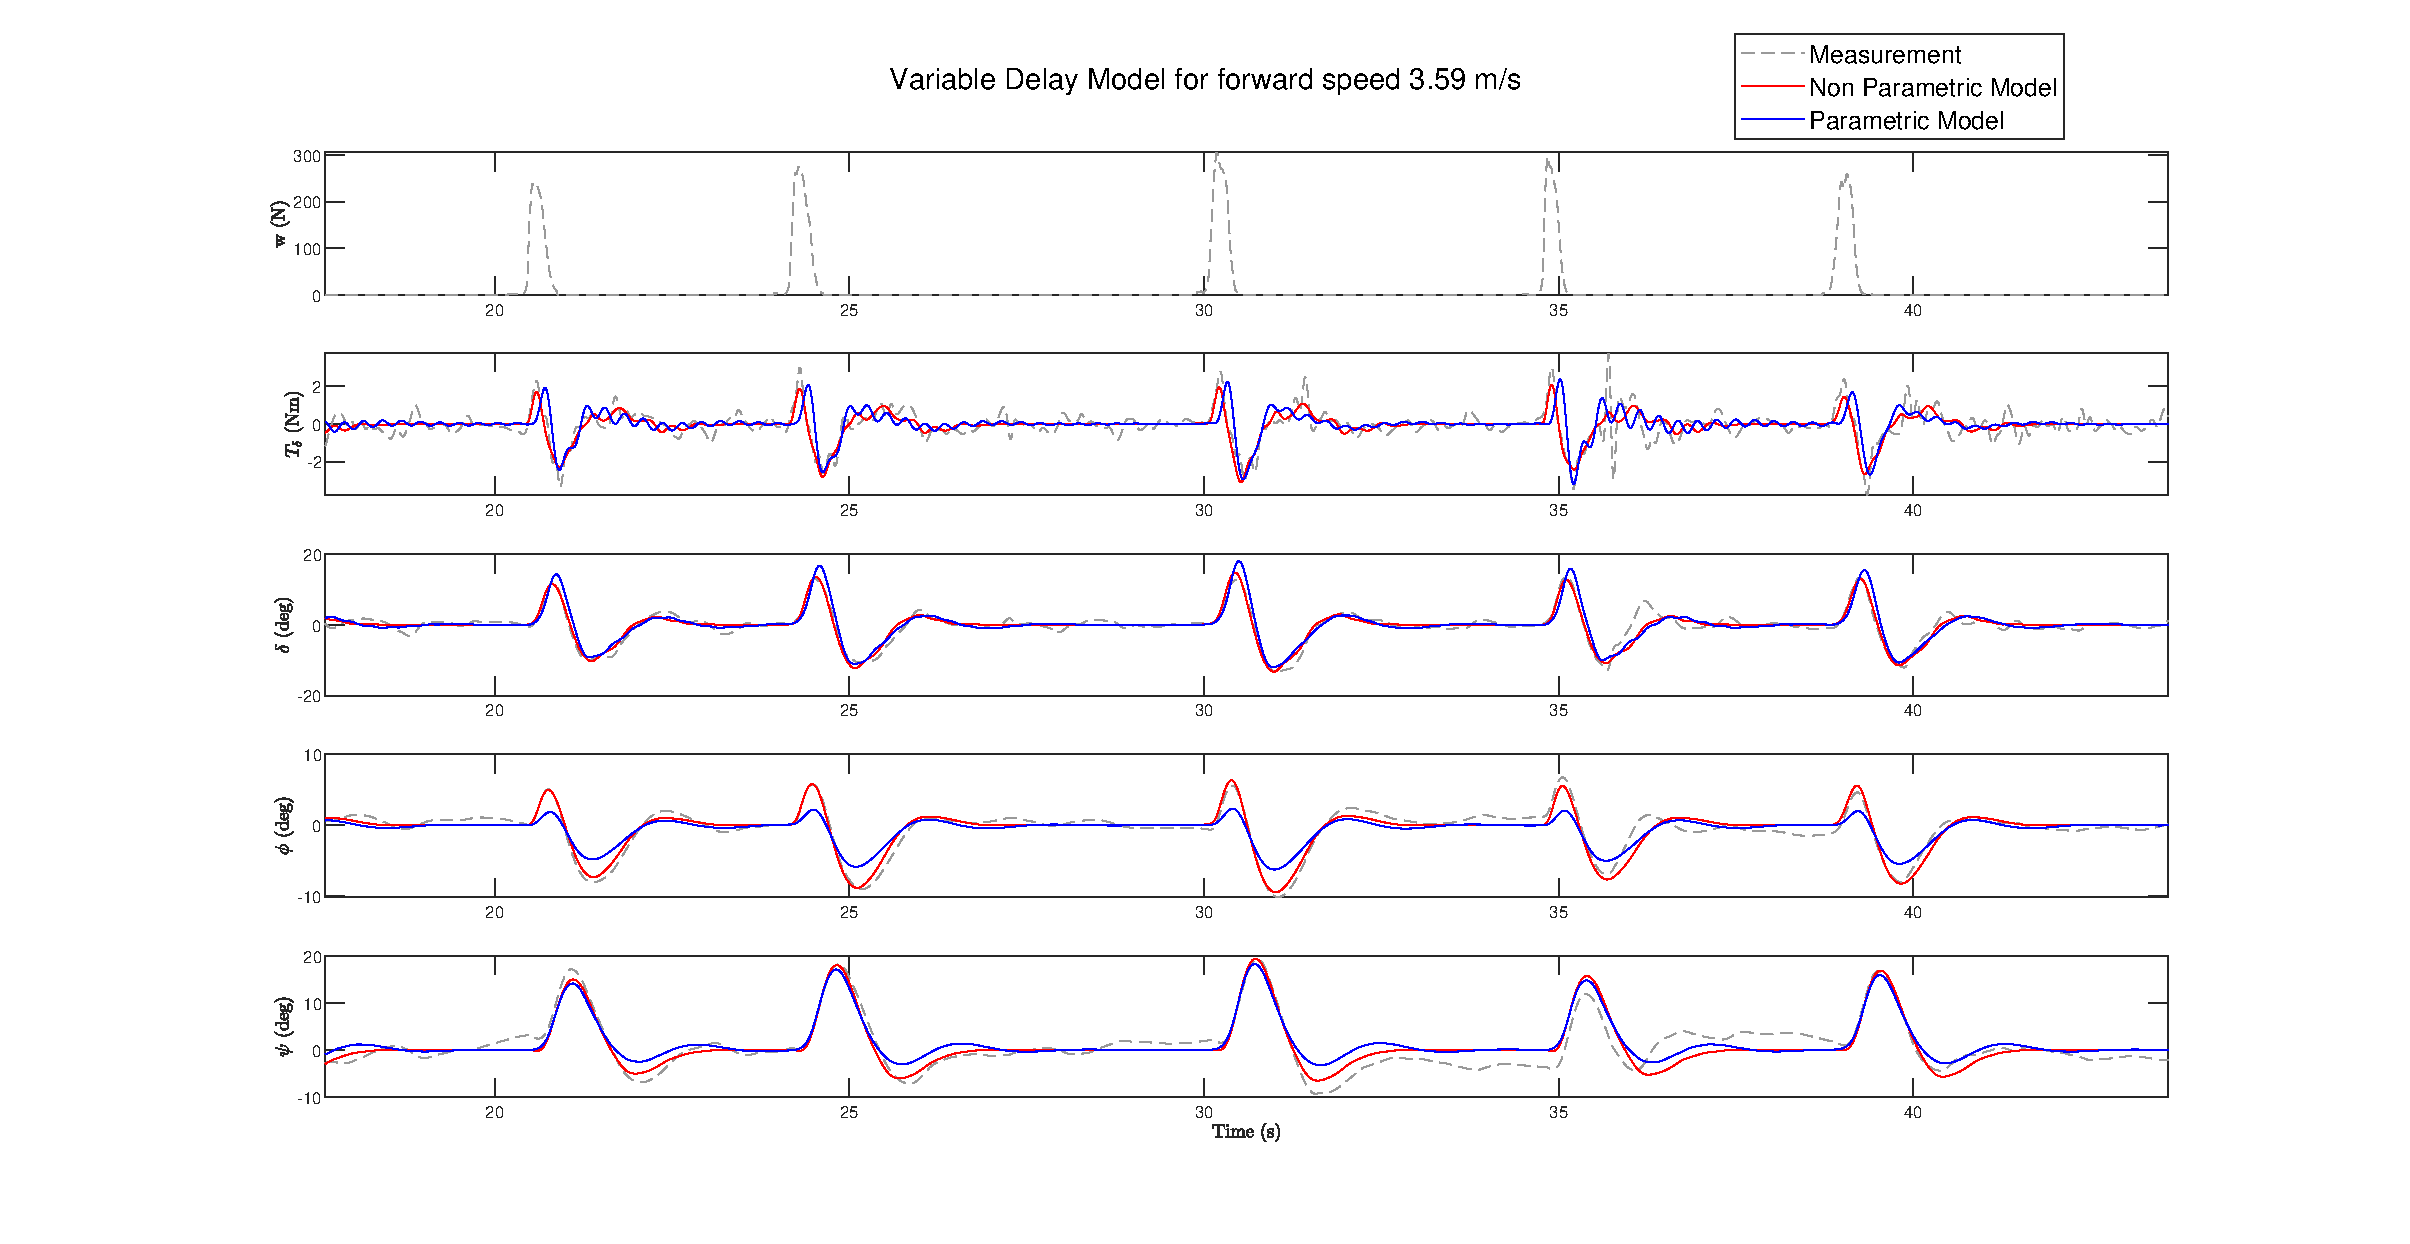
\includegraphics[width=1.4\textwidth]{images/raw_fit_plots/delay_36.eps}}
        \caption{}
        \label{fig:dm_fit2}
    \end{subfigure}
    
    \caption{Comparison between parametric model output (Variable Delay Model), non-parametric model ouput and measured signals for the two lowest speed levels for the case where torque feedback is present in the rider control model and biccyle is operating under the "haptics on" dynamics.}
    \label{fig:dm_fitA}
 \end{figure}

 \begin{figure}
    \centering
    \begin{subfigure}[b]{\textwidth}
        \centering
        \makebox[\textwidth][c]{ 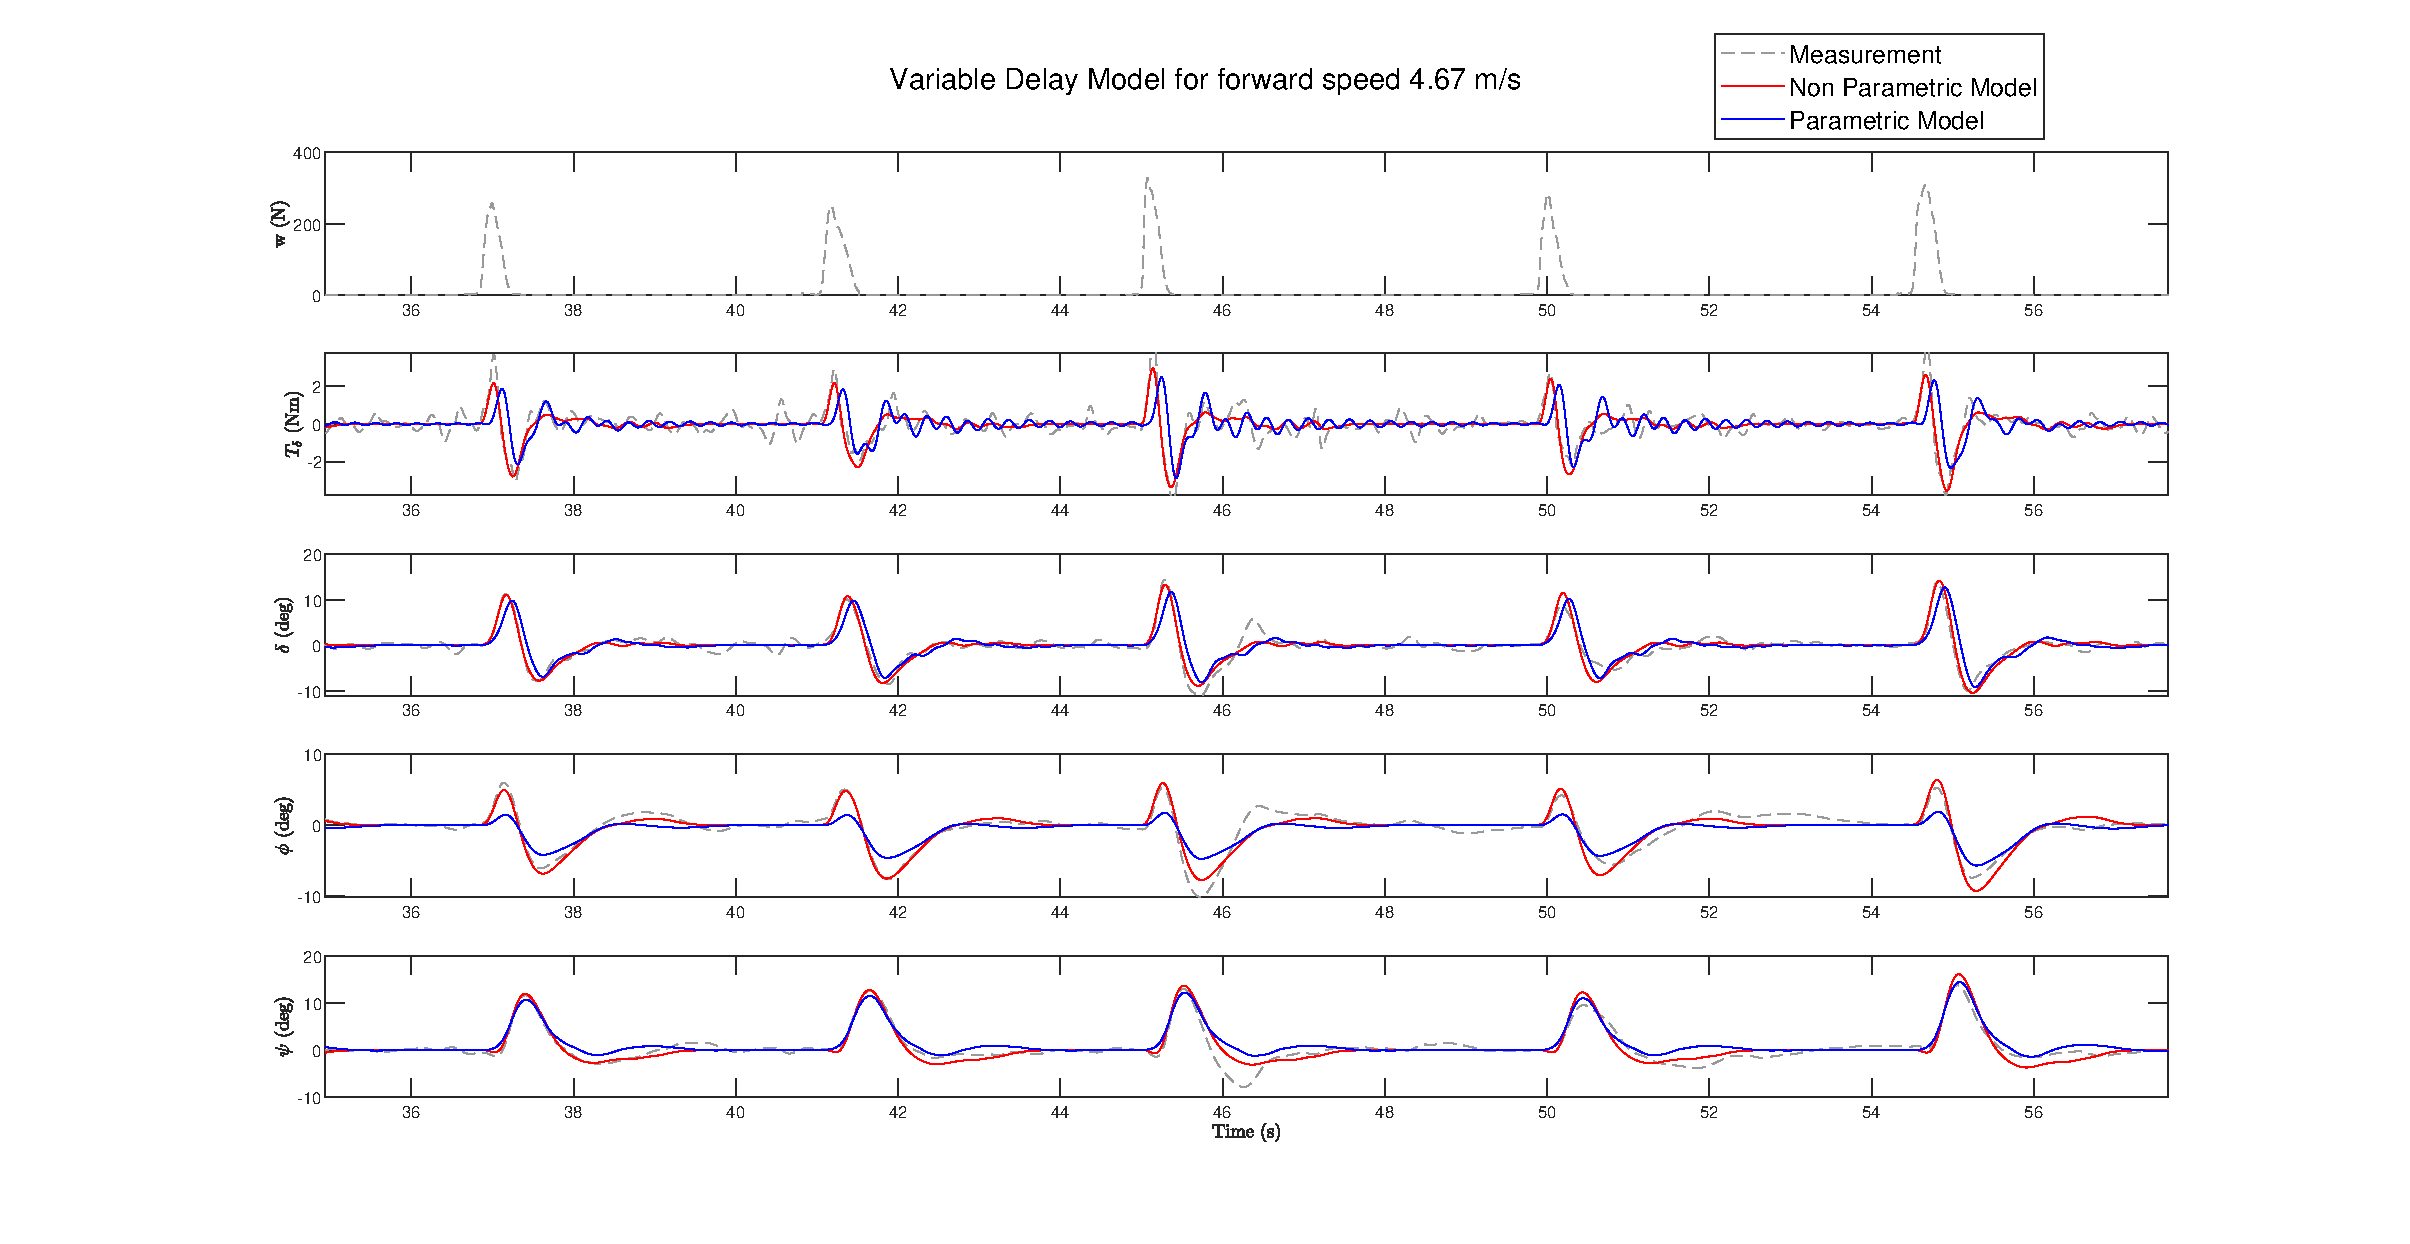
\includegraphics[width=1.4\textwidth]{images/raw_fit_plots/delay_46.eps}}
        \caption{}
        \label{fig:dm_fit3}
    \end{subfigure}
    \begin{subfigure}[b]{\textwidth}
        \centering
        \makebox[\textwidth][c]{ \includegraphics[width=1.4\textwidth]{images/raw_fit_plots/delay_57.eps}}
        \caption{}
        \label{fig:dm_fit4}
    \end{subfigure}
    
    \caption{Comparison between parametric model output (Variable Delay Model), non-parametric model ouput and measured signals for the two highest speed levels for the case where torque feedback is present in the rider control model and biccyle is operating under the "haptics on" dynamics.}
    \label{fig:dm_fitB}
 \end{figure}

\begin{figure}[!h]
    \centering
    \captionsetup{justification=centering,margin=2cm}

    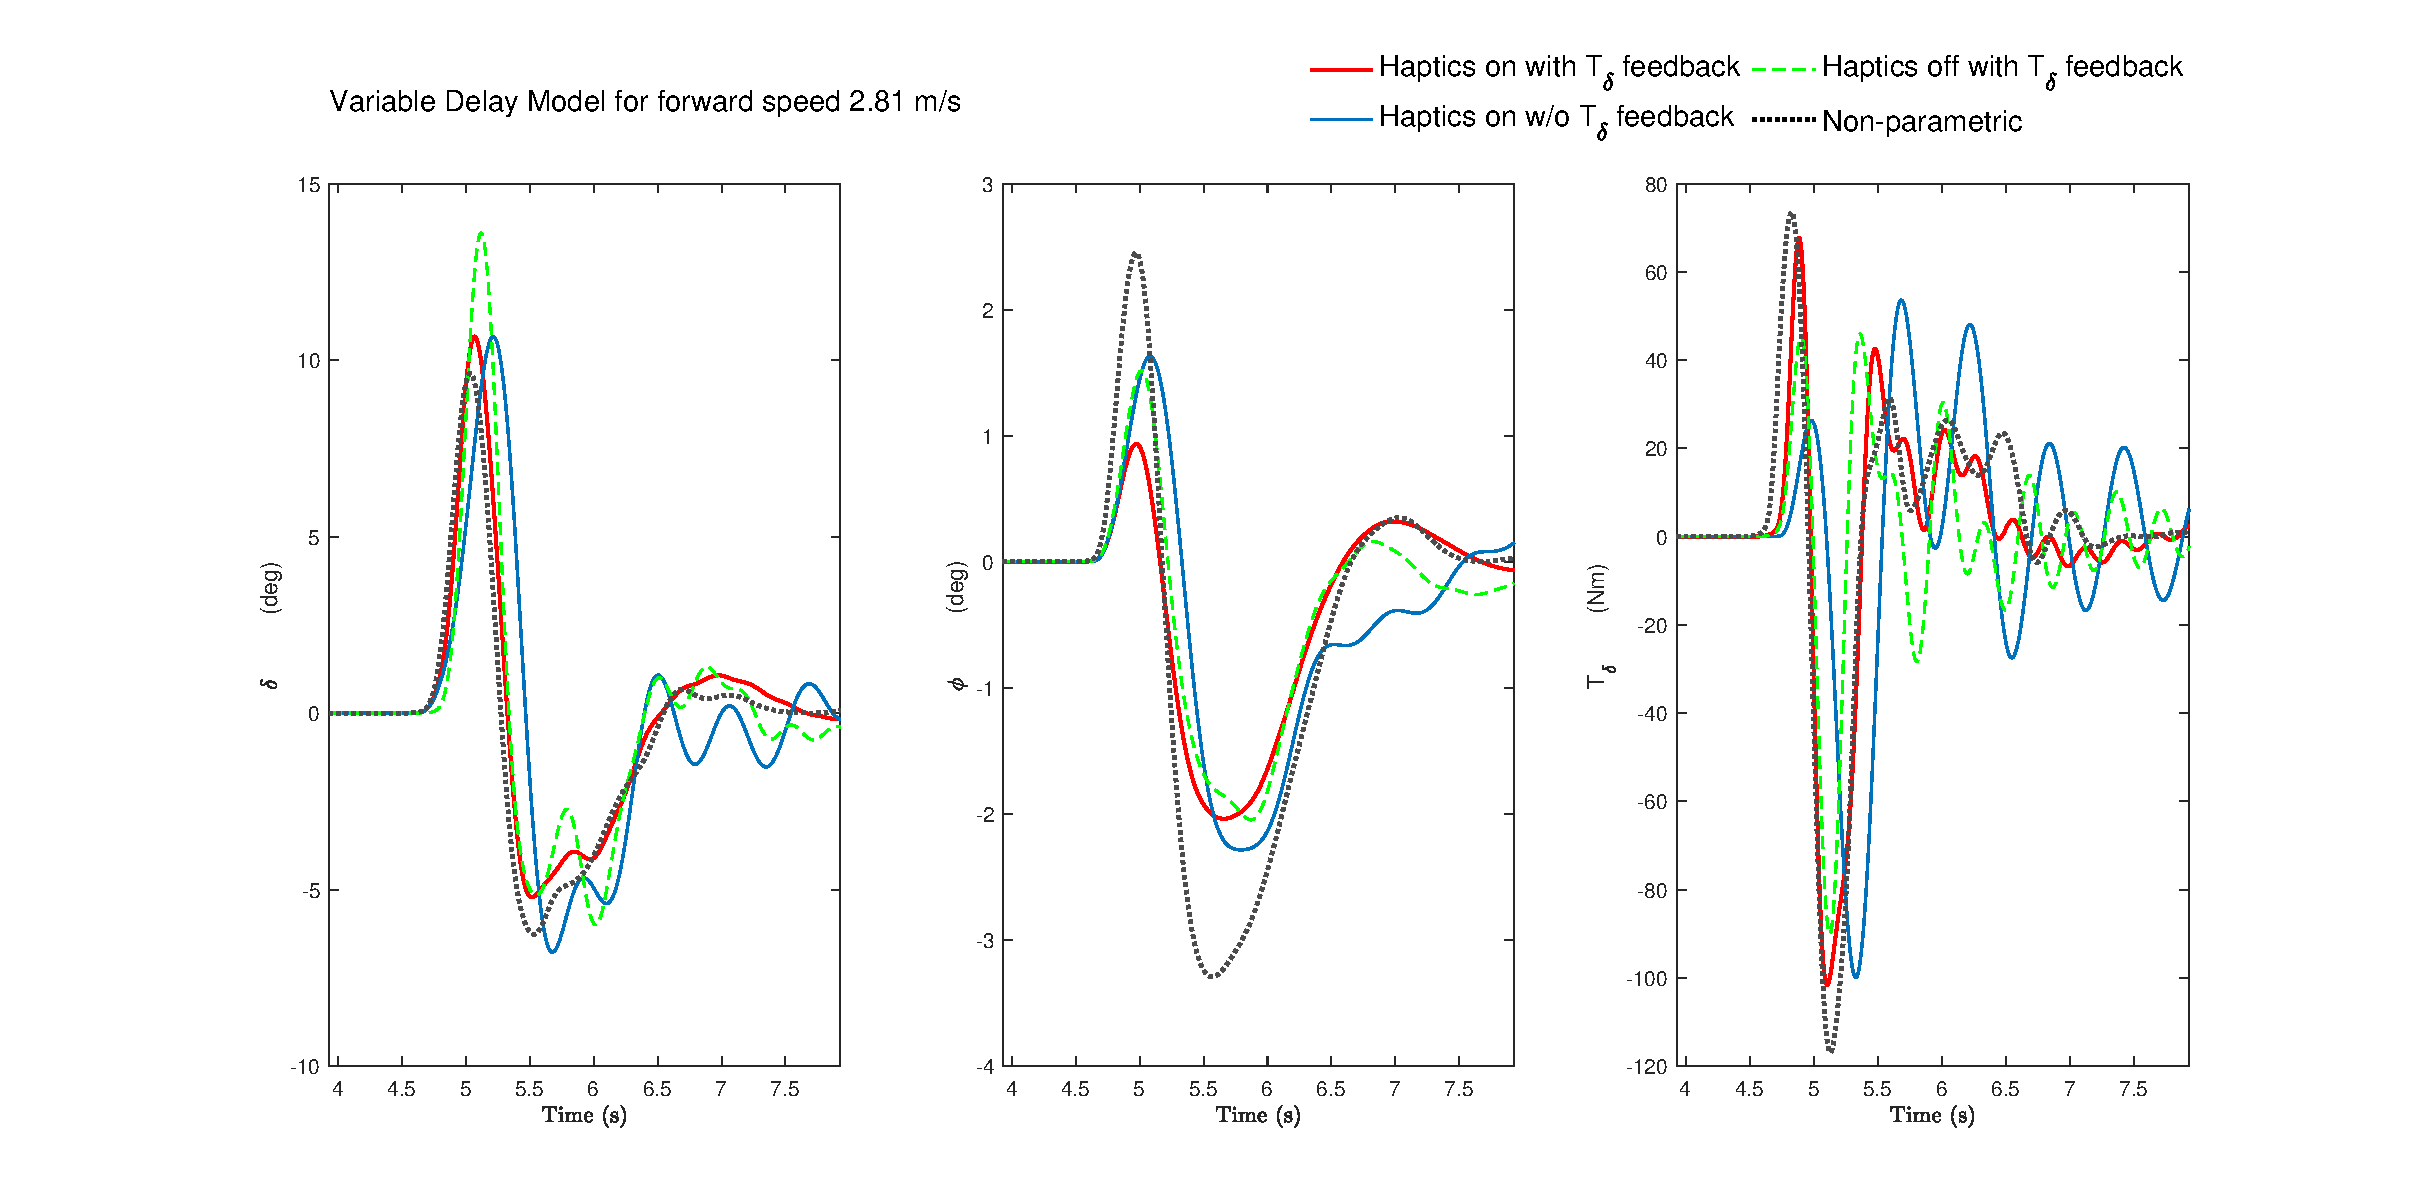
\includegraphics[width=\textwidth]{images/fb_compare_plots/delay_fb_compare28.eps}
    \caption{Steering, roll angle and input rider torque of the median rider compared among torque feedback levels  for the forward speed of 2.81 \si{\meter\per\second} in the Variable Delay Model. Response of the first disturbance in the run is shown.}
    \label{fig:paper8}
\end{figure}


    \subsection{Reafferent Optimal Prediction  Model}

The ROP model of  \cref{fig:paper4} is implemented with a consistent time delay among sensory pathways equal to 50 \si{\milli\second}. Adaptation of the predictor to work with variable time delays is not part of the scope of this work. It is assumed that the internal model of bicycle and neuromuscular dynamics along with the internal model of the inherent time delay responsible for prediction is perfect for controlling the normal bicycle dynamics (\ensuremath{A^*=A_m^*}). However in the haptics off case, where the steering dynamics change, the internal model is not updated in simulation on purpose. This falls inline with what was noted during the experiments where the subjects adapted to the new bicycle dynamics instantaneously, so a full "re-calibration" of the forward model is too far fetched. This way the extent to which the smith prediction principle can counter forward model inaccuracies is also tested. 


The optimization results for the ROP model are presented in \cref{tb:predict} for the median rider. From the \ensuremath{\mathit{VAF}s} and the signals shown in \cref{fig:ropm_fitA,fig:ropm_fitB} it is visible that the quality of the fit is comparable with the ideal zero delay case. In the haptics on with \ensuremath{K_{T_\delta}} feedback condition no significant difference between CVs is noticed, however similar drop in \ensuremath{\mathit{VAF}_\delta} is present as in the zero delay model when  \ensuremath{K_{T_\delta}} feedback is turned off, which indicates significant importance of the golgi tendon organ sensory pathway. In the haptics on without \ensuremath{K_{T_\delta}} feedback case, the gain \ensuremath{K_{\delta}} shows improportionally bigger uncertainty (see \cref{tb:predict}). Furthermore, the steering response exhibits  the same oscillatory behaviour when torque feedback is completely disabled (see \cref{fig:paper10} ). However, the predictor manages to compensate in the haptics off case and achieve good fit which is not present in the variable delay model. In \cref{fig:gains_speed} the gains estimated for the median rider as a function of speed for all torque feedback conditions are presented. Consistent trends could only be discerned for the heading proportional gain \ensuremath{K_\psi}.

\begin{figure}[!h]
    \centering
    \begin{subfigure}[b]{\textwidth}
        \centering
        \makebox[\textwidth][c]{ 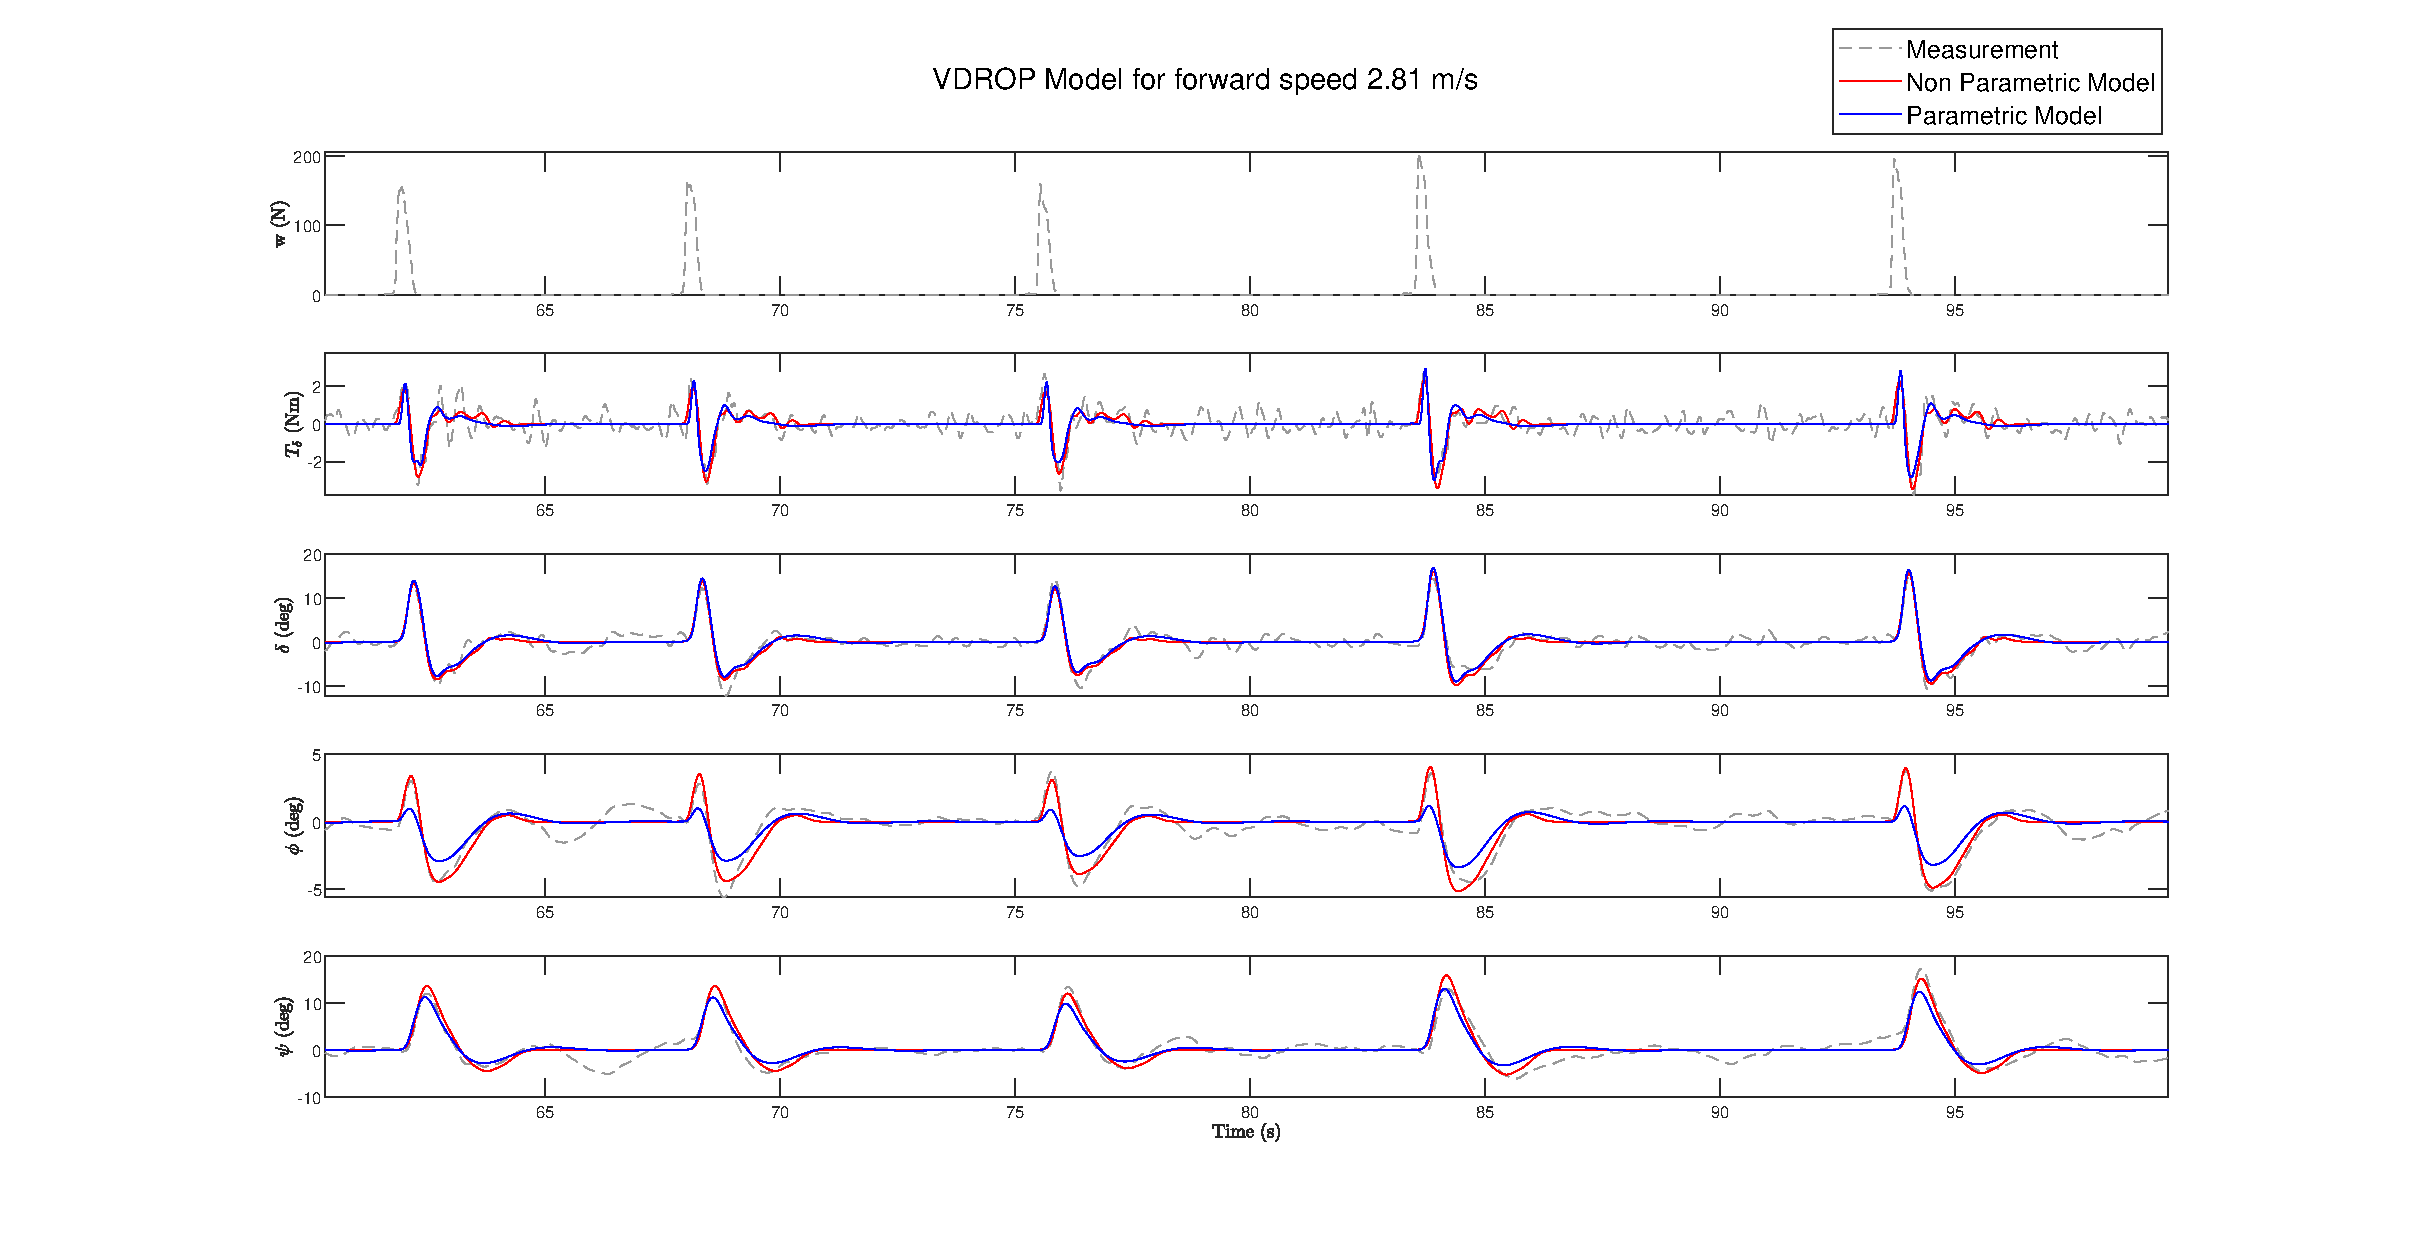
\includegraphics[width=1.4\textwidth]{images/raw_fit_plots/predict_28.eps}}
        \caption{}
        \label{fig:ropm_fit1}
    \end{subfigure}
    \begin{subfigure}[b]{\textwidth}
        \centering
        \makebox[\textwidth][c]{ 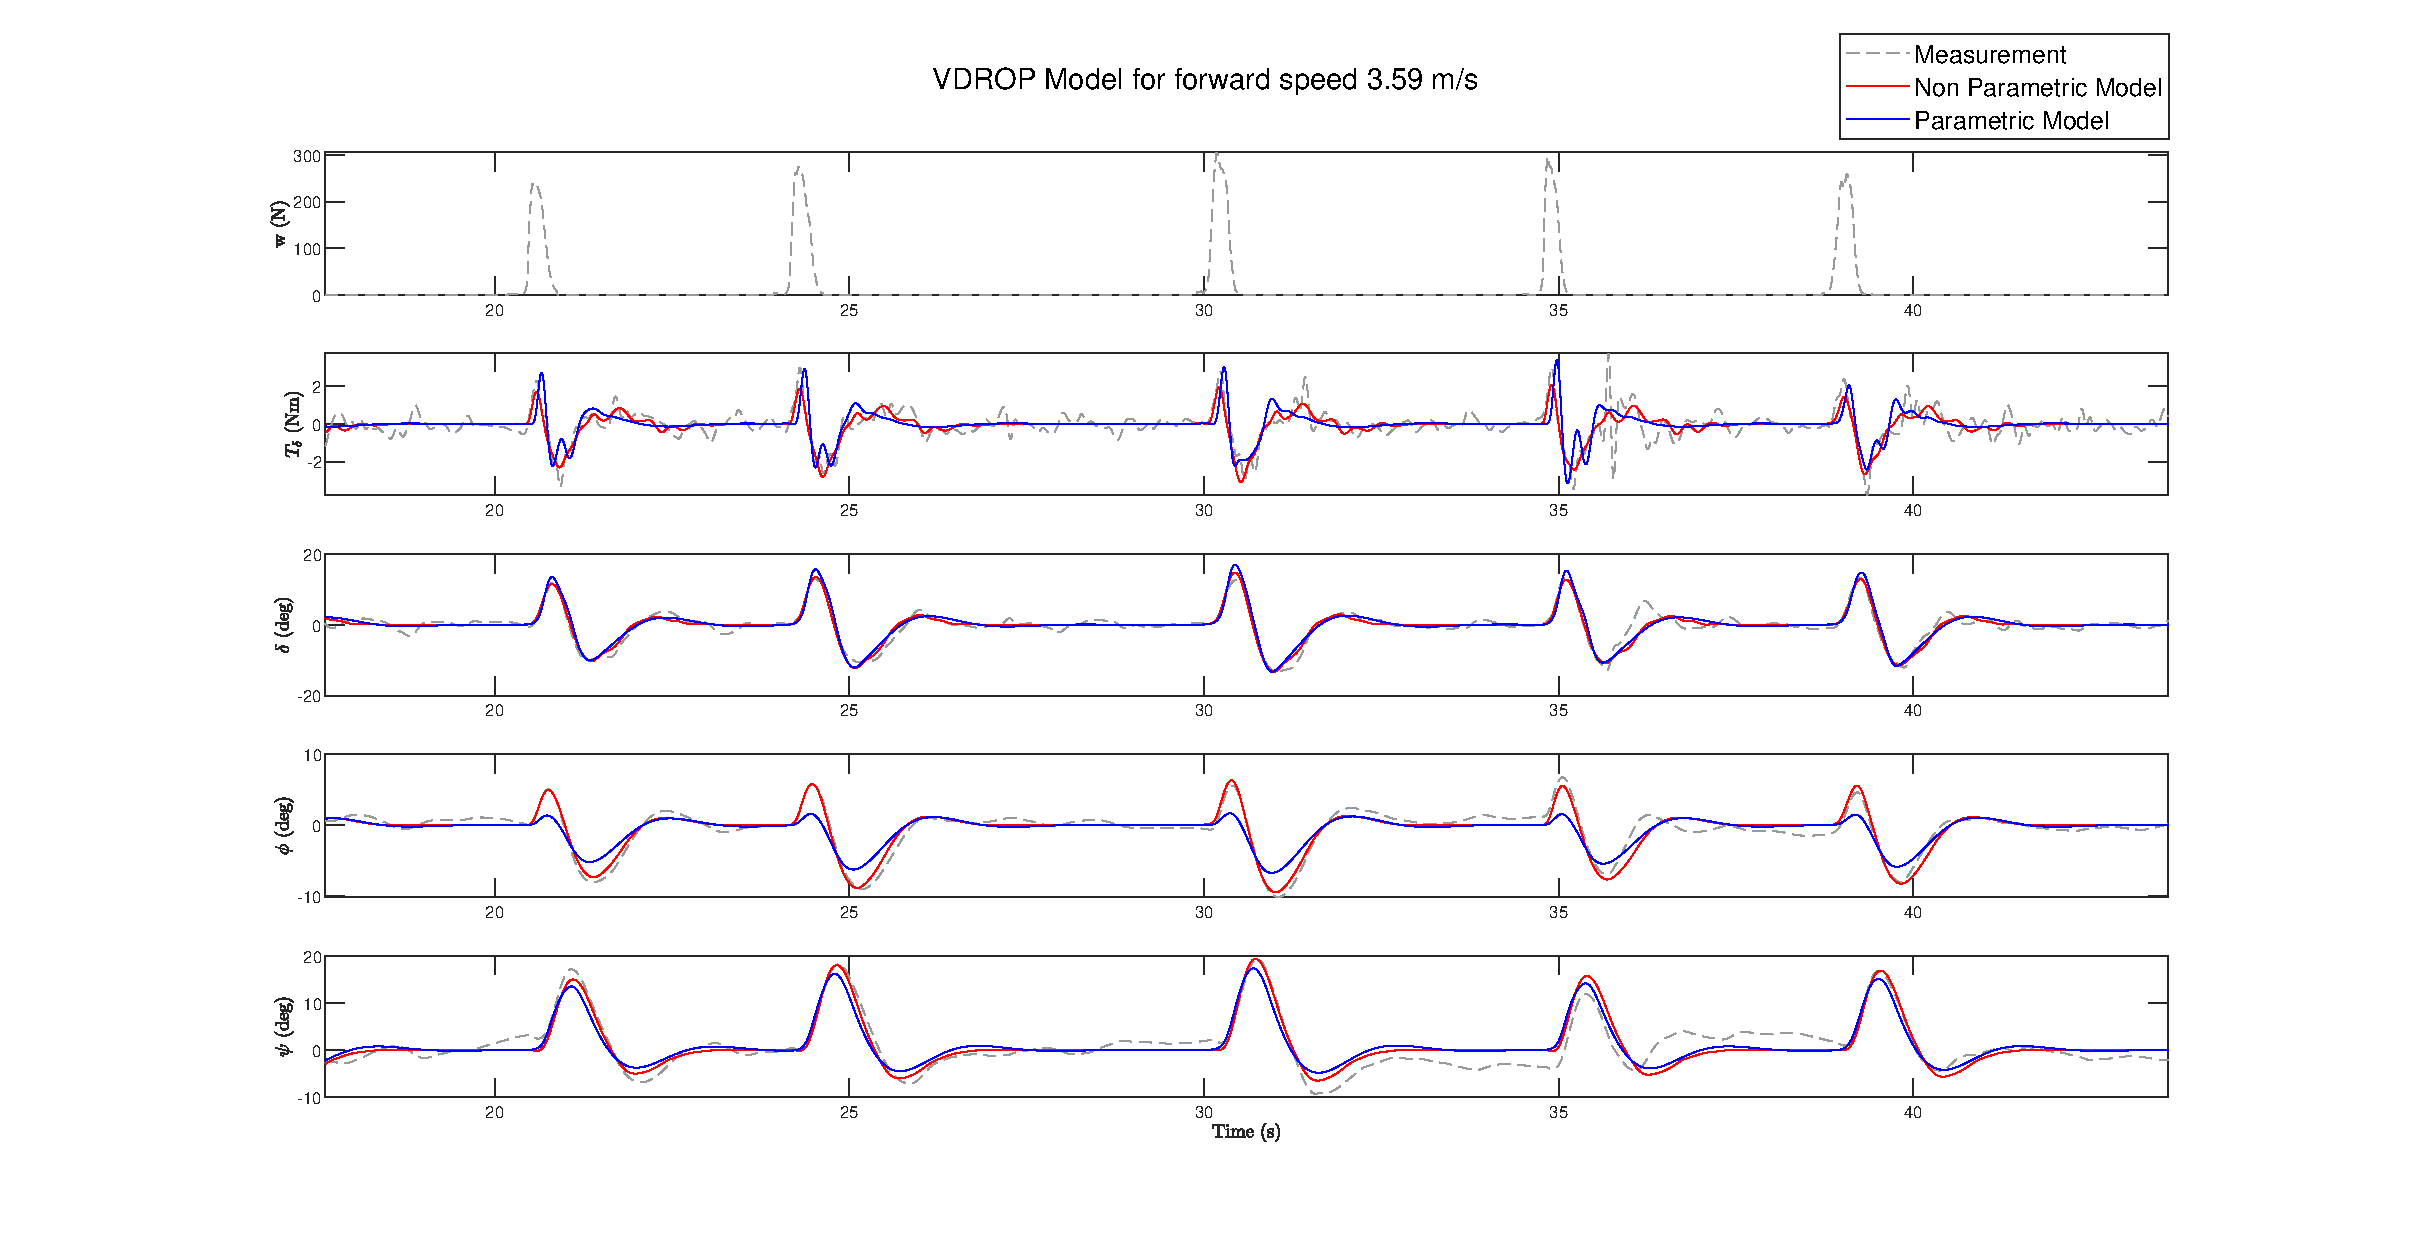
\includegraphics[width=1.4\textwidth]{images/raw_fit_plots/predict_36.eps}}
        \caption{}
        \label{fig:ropm_fit2}
    \end{subfigure}
    
    \caption{Comparison between parametric model output (ROP Model), non-parametric model ouput and measured signals for the two lowest speed levels for the case where torque feedback is present in the rider control model and biccyle is operating under the "haptics on" dynamics.}
    \label{fig:ropm_fitA}
 \end{figure}

 \begin{figure}
    \centering
    \begin{subfigure}[b]{\textwidth}
        \centering
        \makebox[\textwidth][c]{ 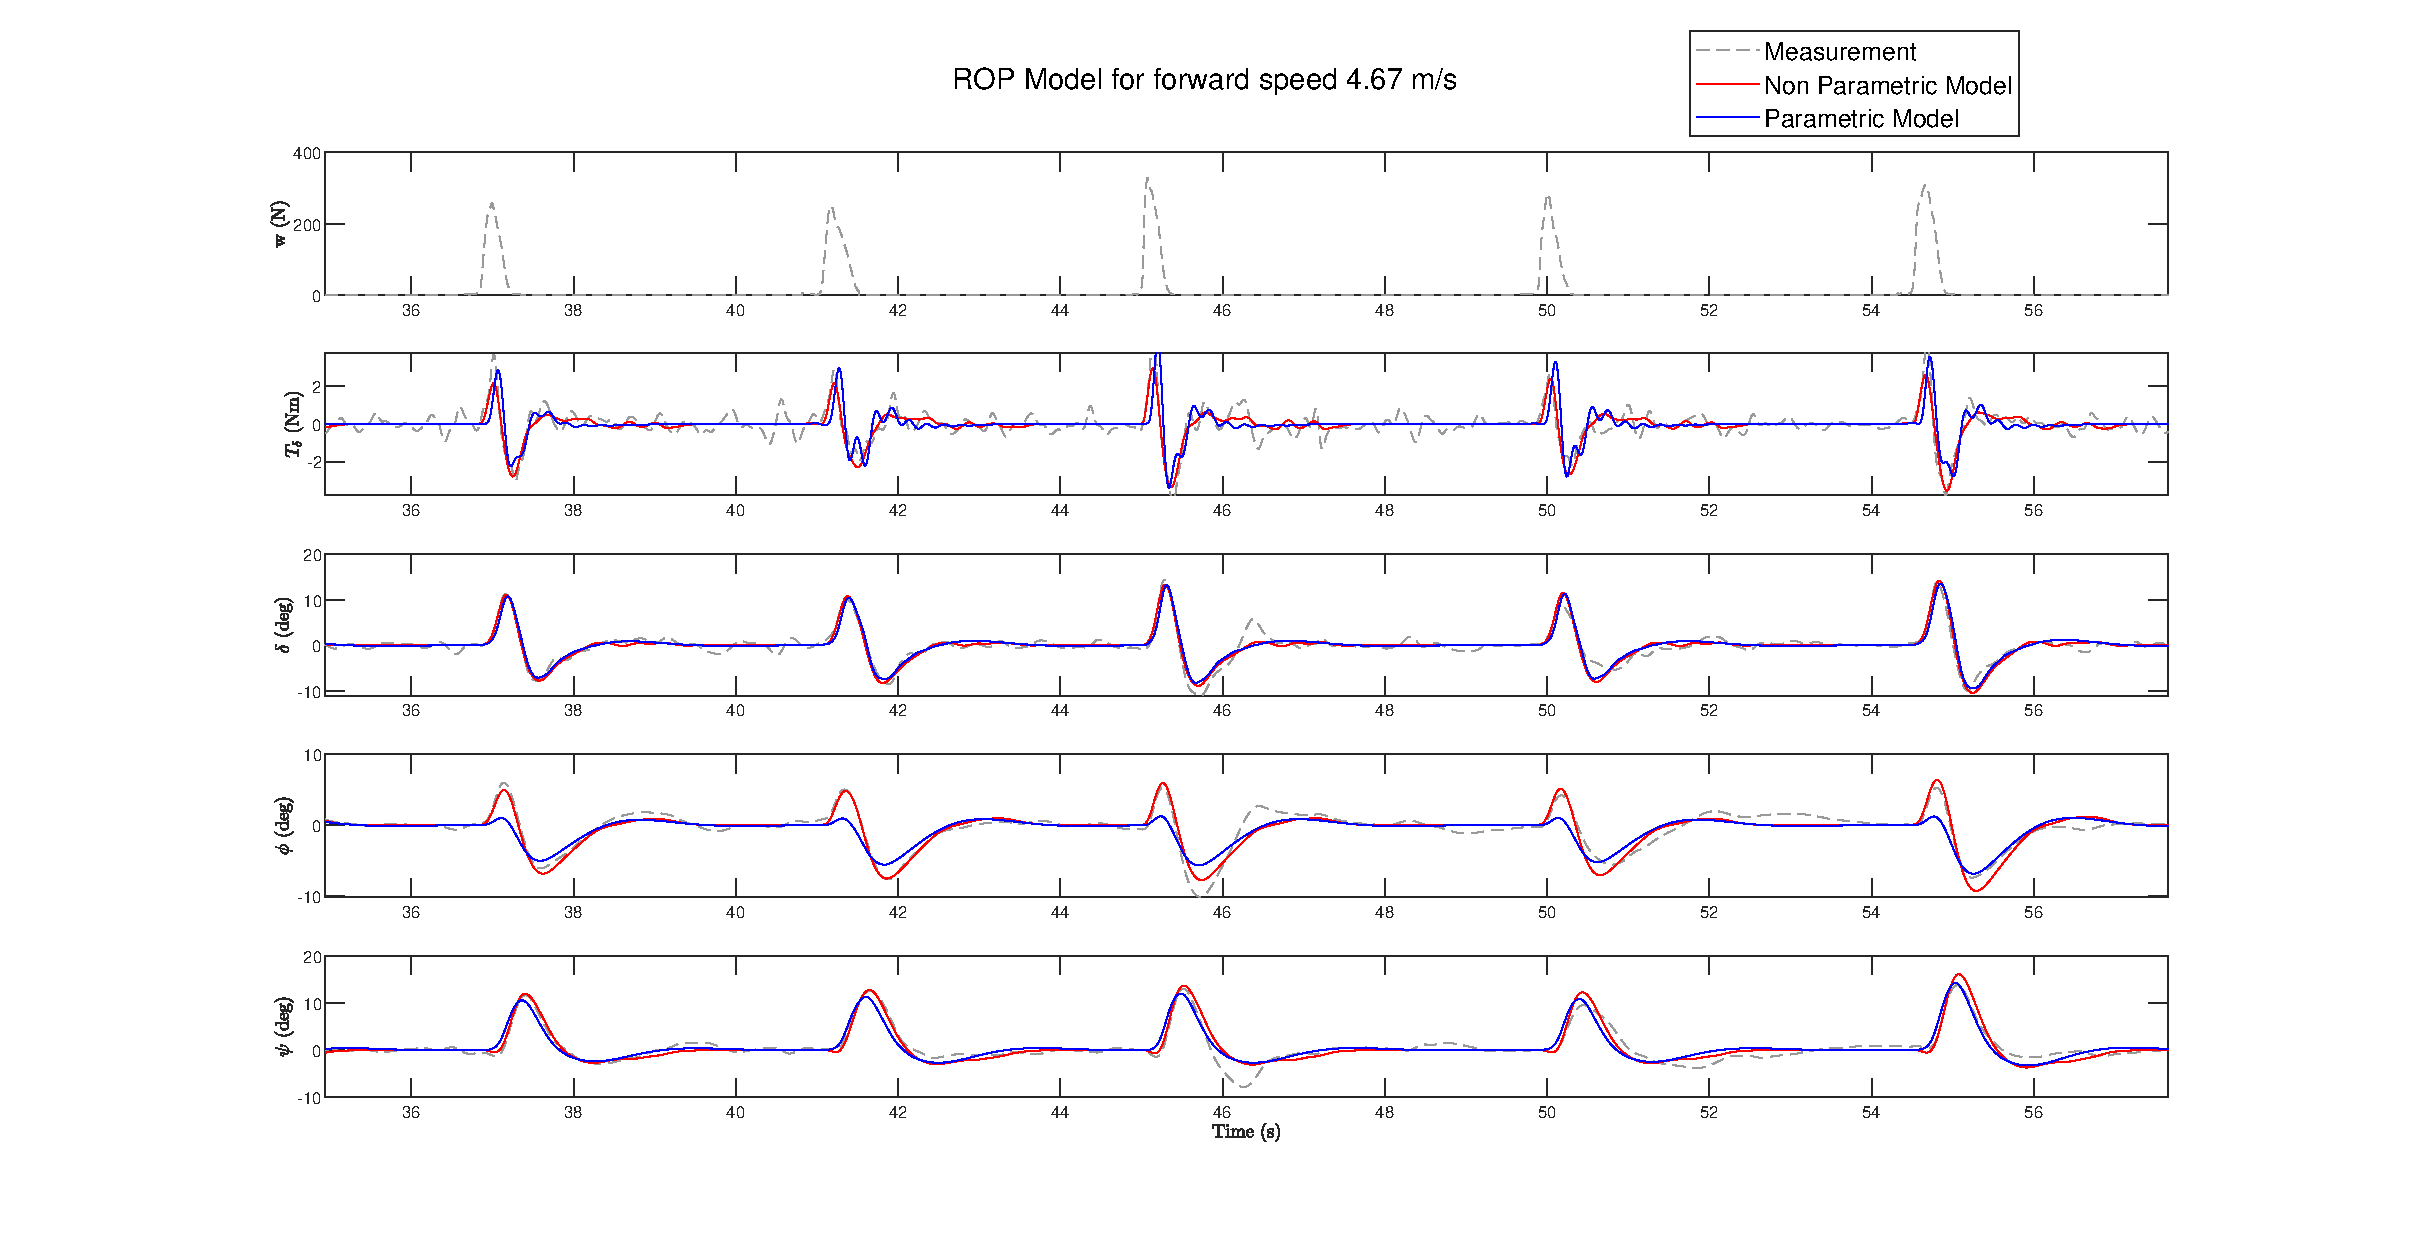
\includegraphics[width=1.4\textwidth]{images/raw_fit_plots/predict_46.eps}}
        \caption{}
        \label{fig:ropm_fit3}
    \end{subfigure}
    \begin{subfigure}[b]{\textwidth}
        \centering
        \makebox[\textwidth][c]{ 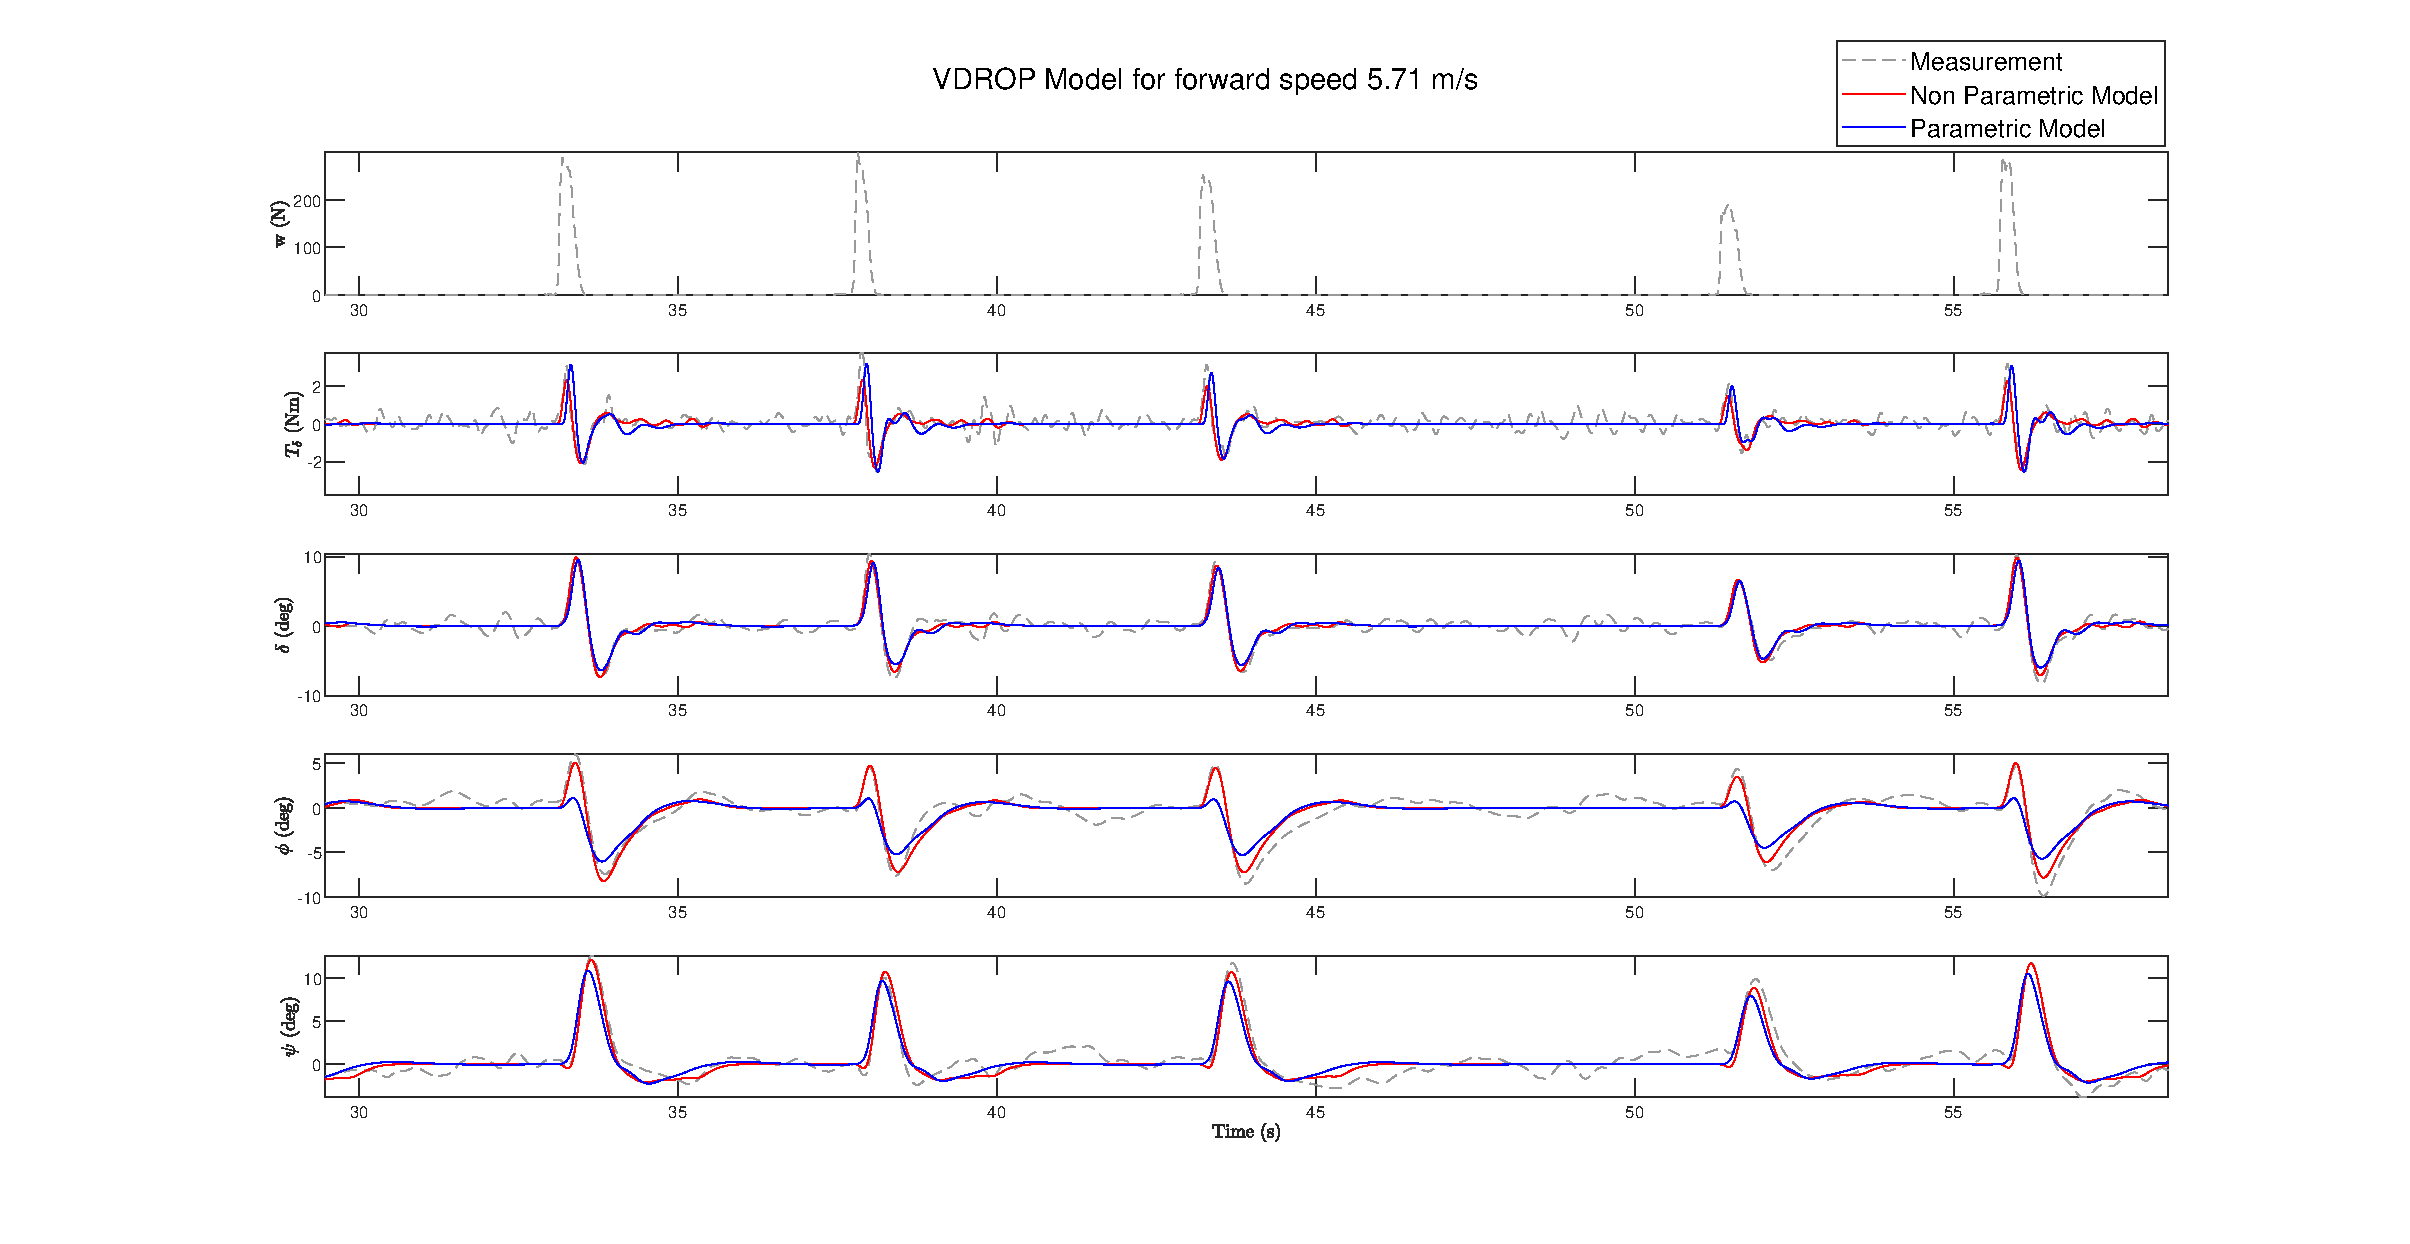
\includegraphics[width=1.4\textwidth]{images/raw_fit_plots/predict_57.eps}}
        \caption{}
        \label{fig:ropm_fit4}
    \end{subfigure}
    
    \caption{Comparison between parametric model output (ROP Model), non-parametric model ouput and  measured signals for the two highest speed levels for the case where torque feedback is present in the rider control model and biccyle is operating under the "haptics on" dynamics.}
    \label{fig:ropm_fitB}
 \end{figure}


\begin{figure}[!h]
    \centering
    \captionsetup{justification=centering,margin=2cm}

    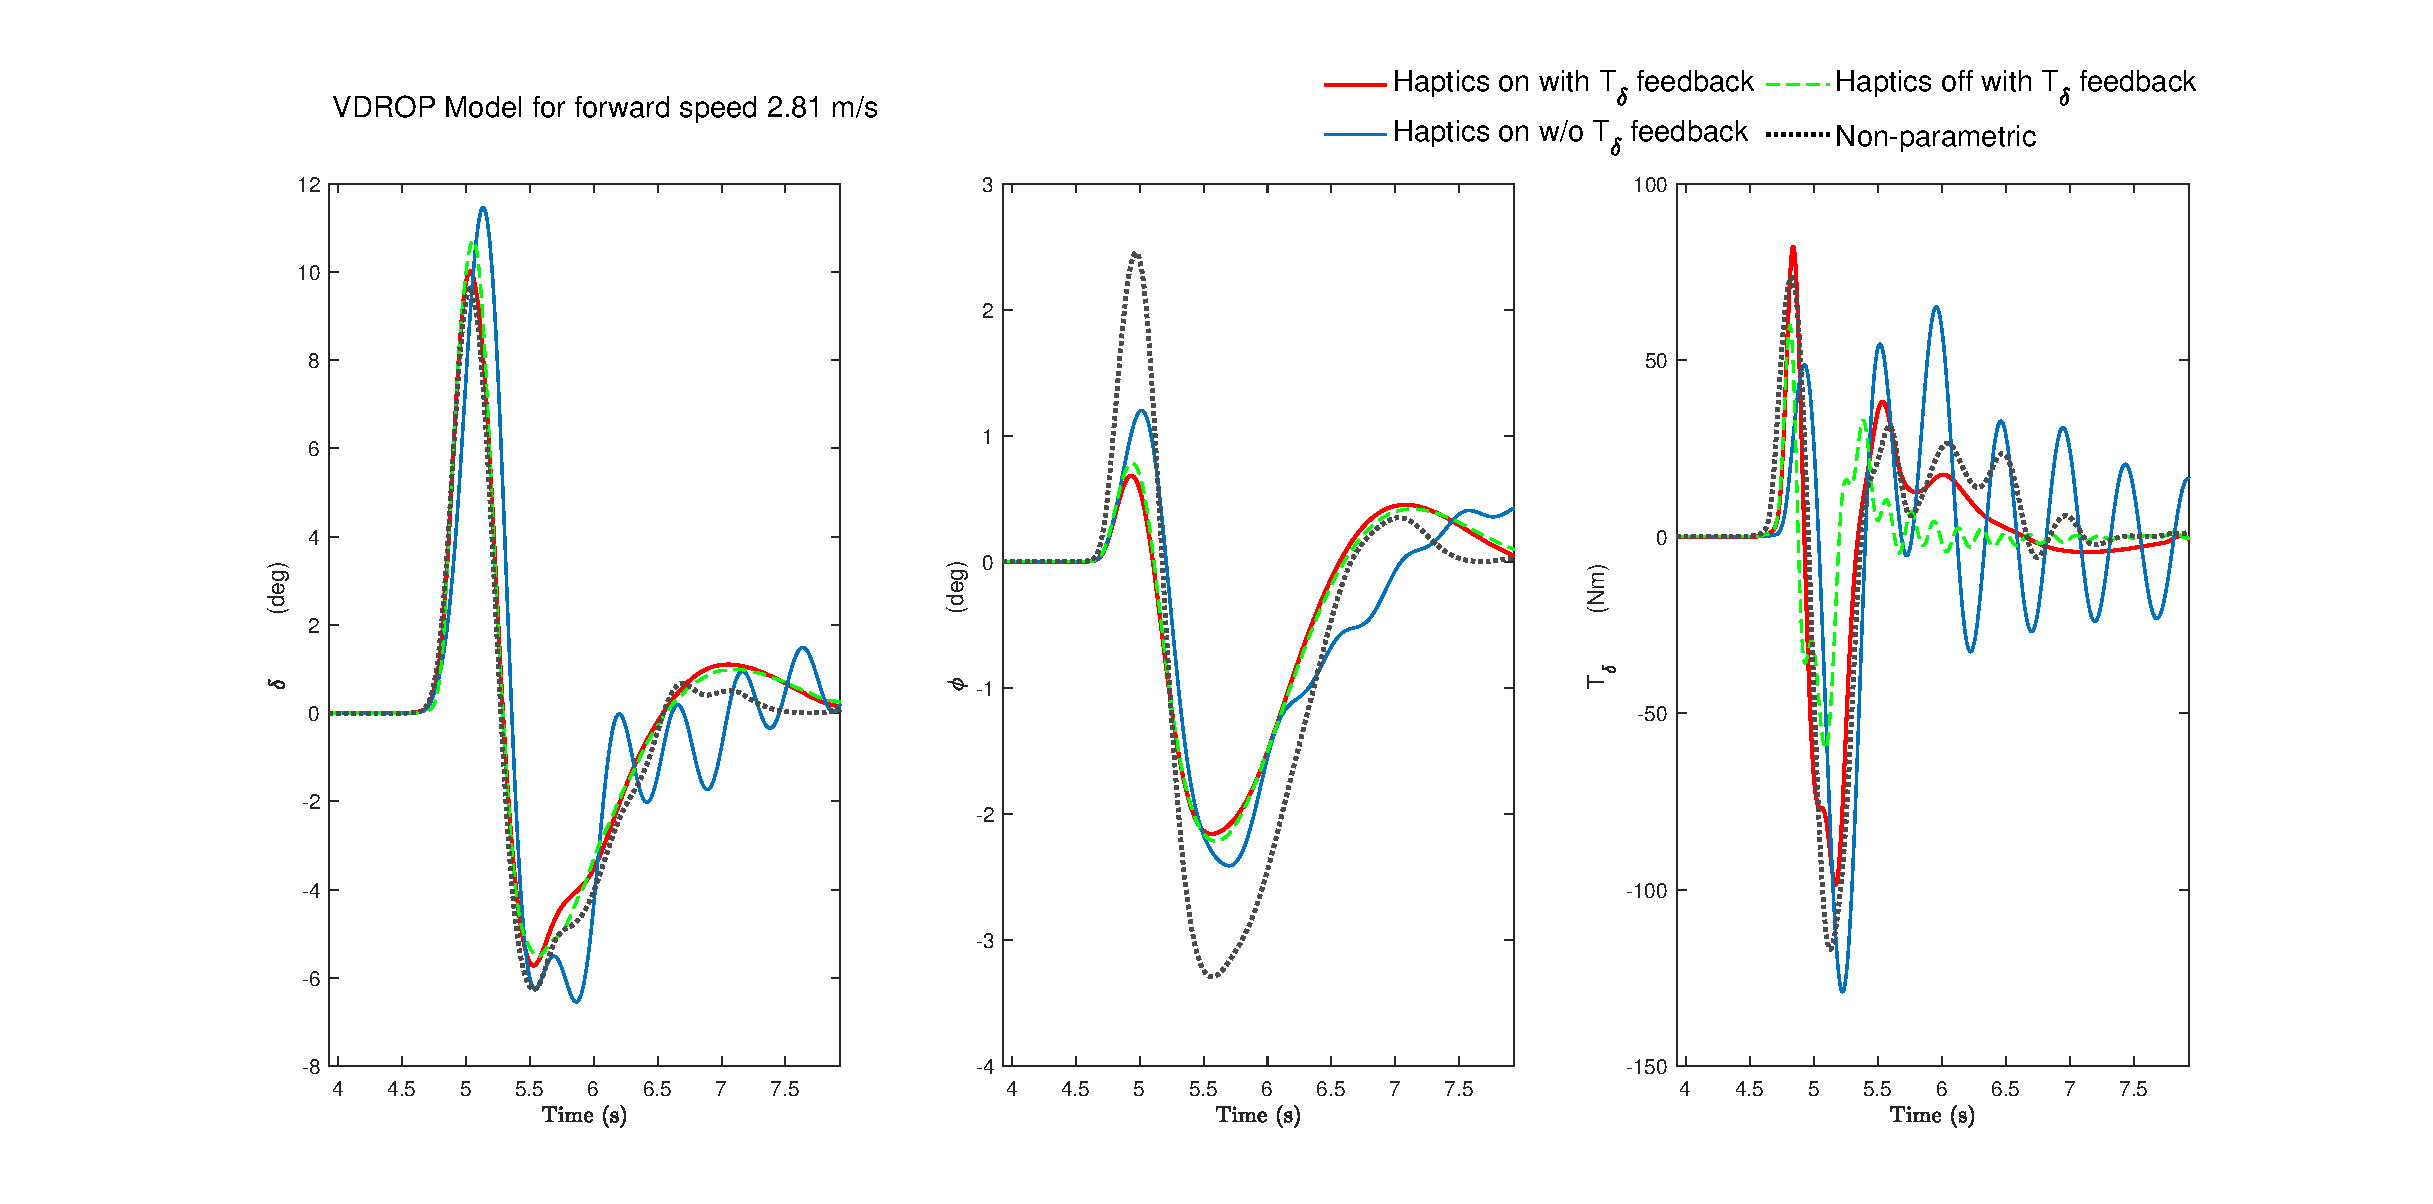
\includegraphics[width=\textwidth]{images/fb_compare_plots/ROP_fb_compare28.eps}
        \caption{Steering, roll angles and input rider torque compared among torque feedback levels  for the forward speed of 2.81 \si{\meter\per\second} in the ROP Model. Response of the first disturbance in the run is shown.}
    \label{fig:paper10}
\end{figure}

In \crefrange{fig:results_compare12}{fig:results_compare34}  a complete comparison between rider models for all feedback conditions is presented. The response shown is the result of the first lateral perturbation of each individual run. The zero delay and prediction models exhibit almost identical responses as it was evident from the over 90\% fit achieved. The variable delay model lags behind in both the produced control input and bicycle output, as is expected. Worth noting the lag in the control input of the prediction model in the first few milliseconds after the perturbation. Despite that fact the ROP model compensates and achieves similar output as the idealized zero delay case. This is a result of the fact that no matter how good the prediction algorithm is the human has no knowledge of the future so the response from the controller will start after the first state information arrives from the feedback pathways which are delayed. The forward model in this case does not help predict the state as it has no information of the external disturbance. 
% Please add the following required packages to your document preamble:
% \usepackage{multirow}





    \begin{figure}
        \centering
        \begin{subfigure}[b]{\textwidth}
            \centering
            \makebox[\textwidth][c]{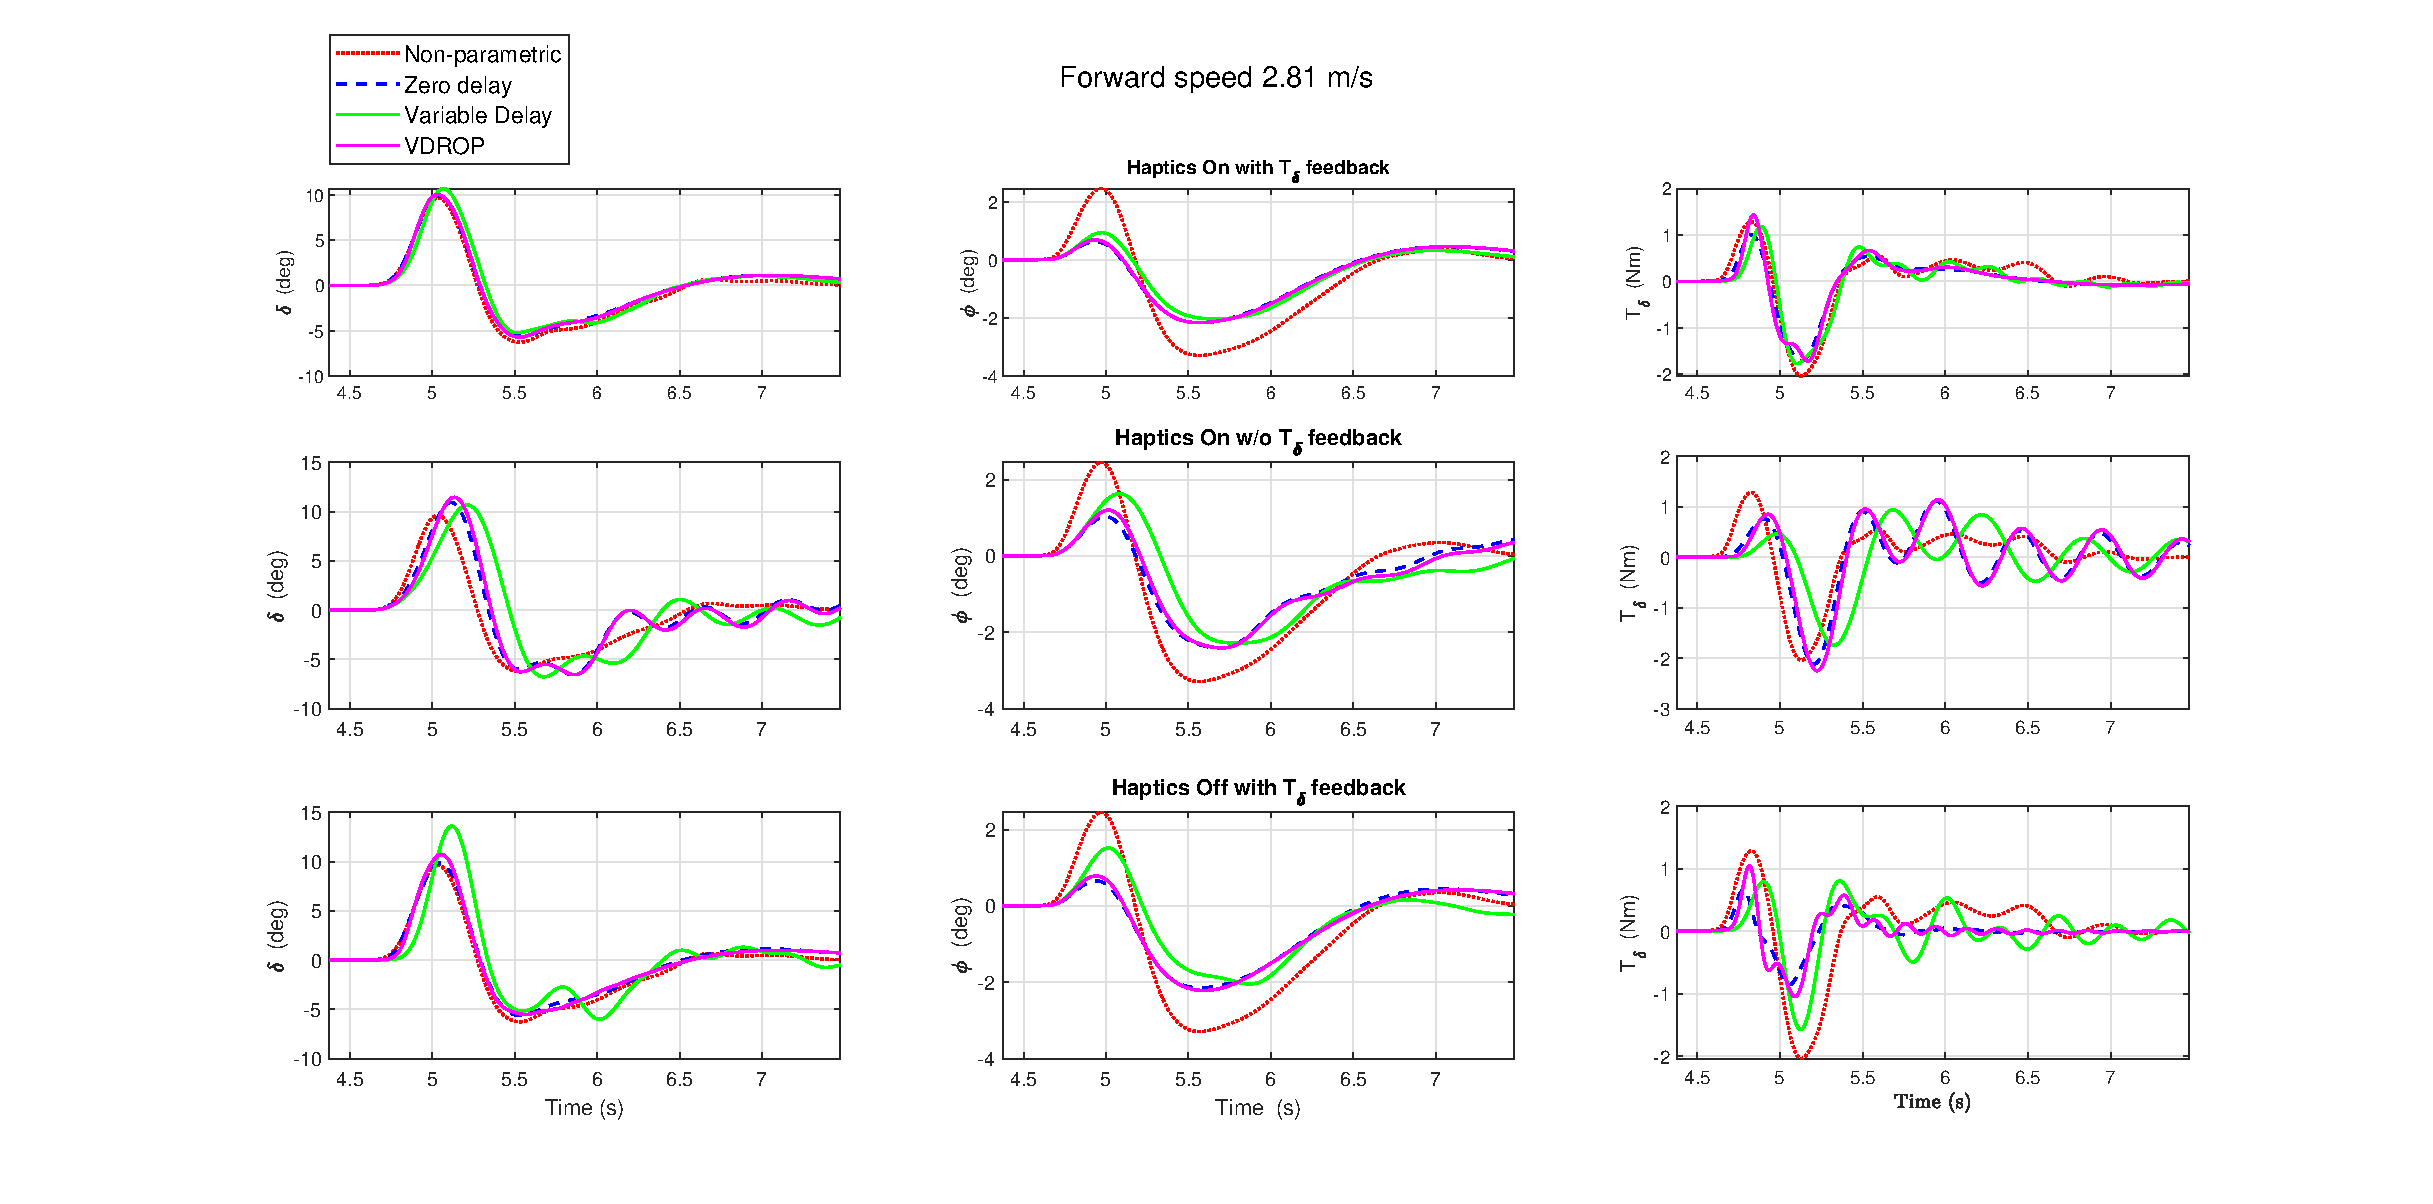
\includegraphics[width=1.1\textwidth]{images/compare_model_plots/compare_models_28.eps}}
            \caption{Comparison between the three rider models for forward speed 2.81 \si{\meter\per\second}}
            \label{fig:results_compare1}
        \end{subfigure}
        \begin{subfigure}[b]{\textwidth}
            \centering
            \makebox[\textwidth][c]{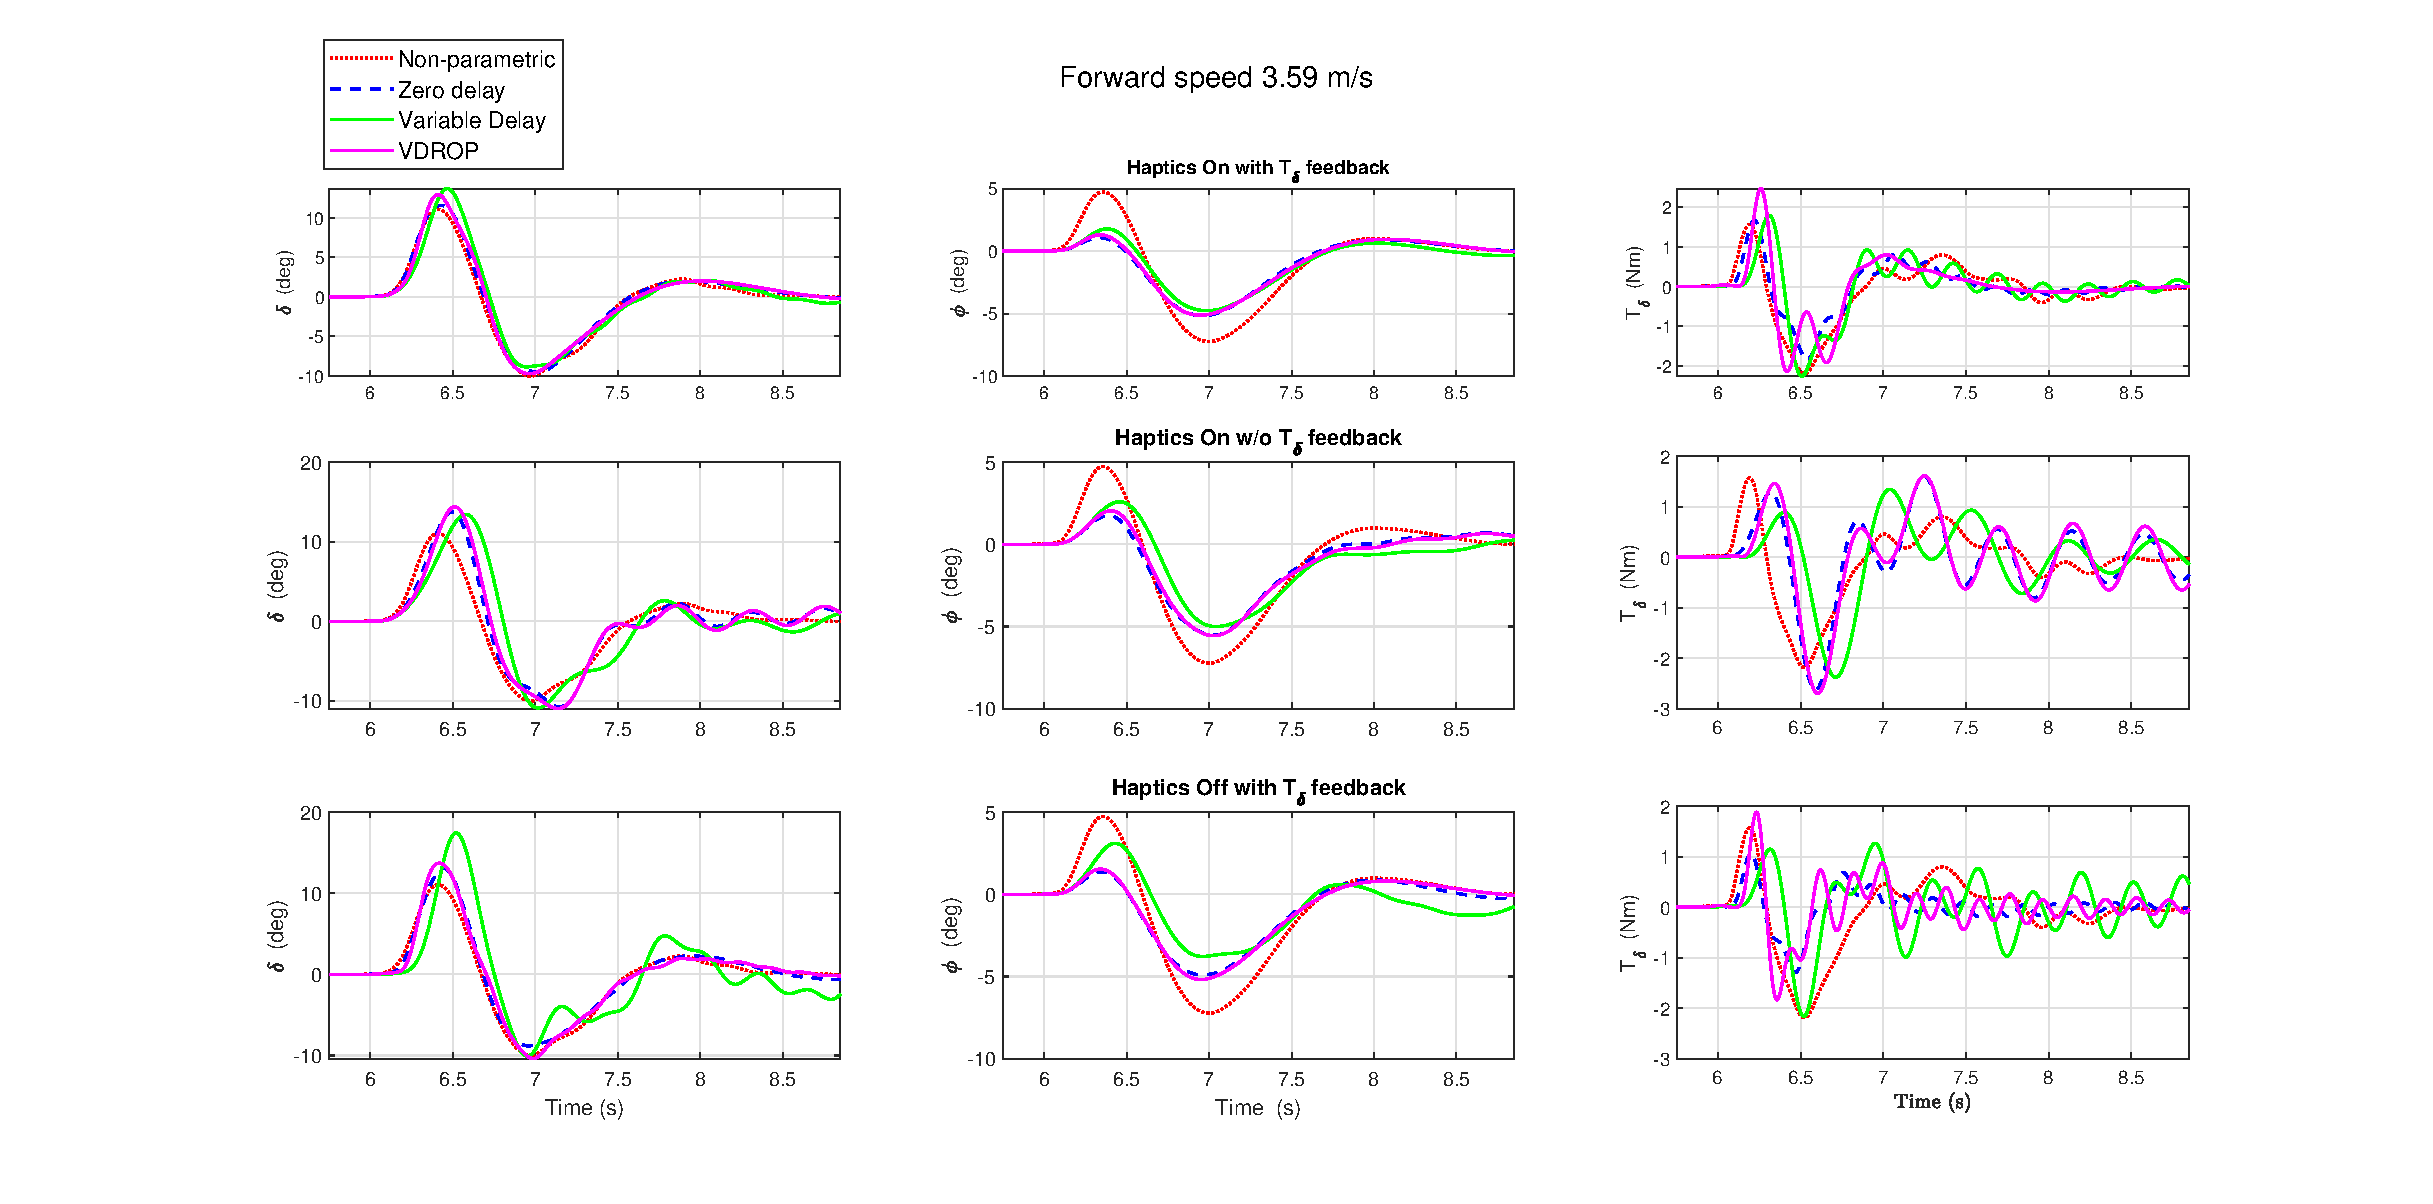
\includegraphics[width=1.1\linewidth]{images/compare_model_plots/compare_models_36.eps}}
            \caption{Comparison between the three rider models for forward speed 3.6 \si{\meter\per\second}}            
            \label{fig:results_compare2}
        \end{subfigure}
        \caption{Steering angle \ensuremath{\delta}, roll angle \ensuremath{\phi} and steering torque \ensuremath{T_\delta} compared among the three rider models implemented for all torque feedback conditions, for the two lowest speed levels for the response of the median rider to the first perturbation of each run. Non parametric output included for reference.}
        \label{fig:results_compare12}
     \end{figure}



     \begin{figure}
        \centering
        \begin{subfigure}[b]{\textwidth}
            \centering
            \makebox[\textwidth][c]{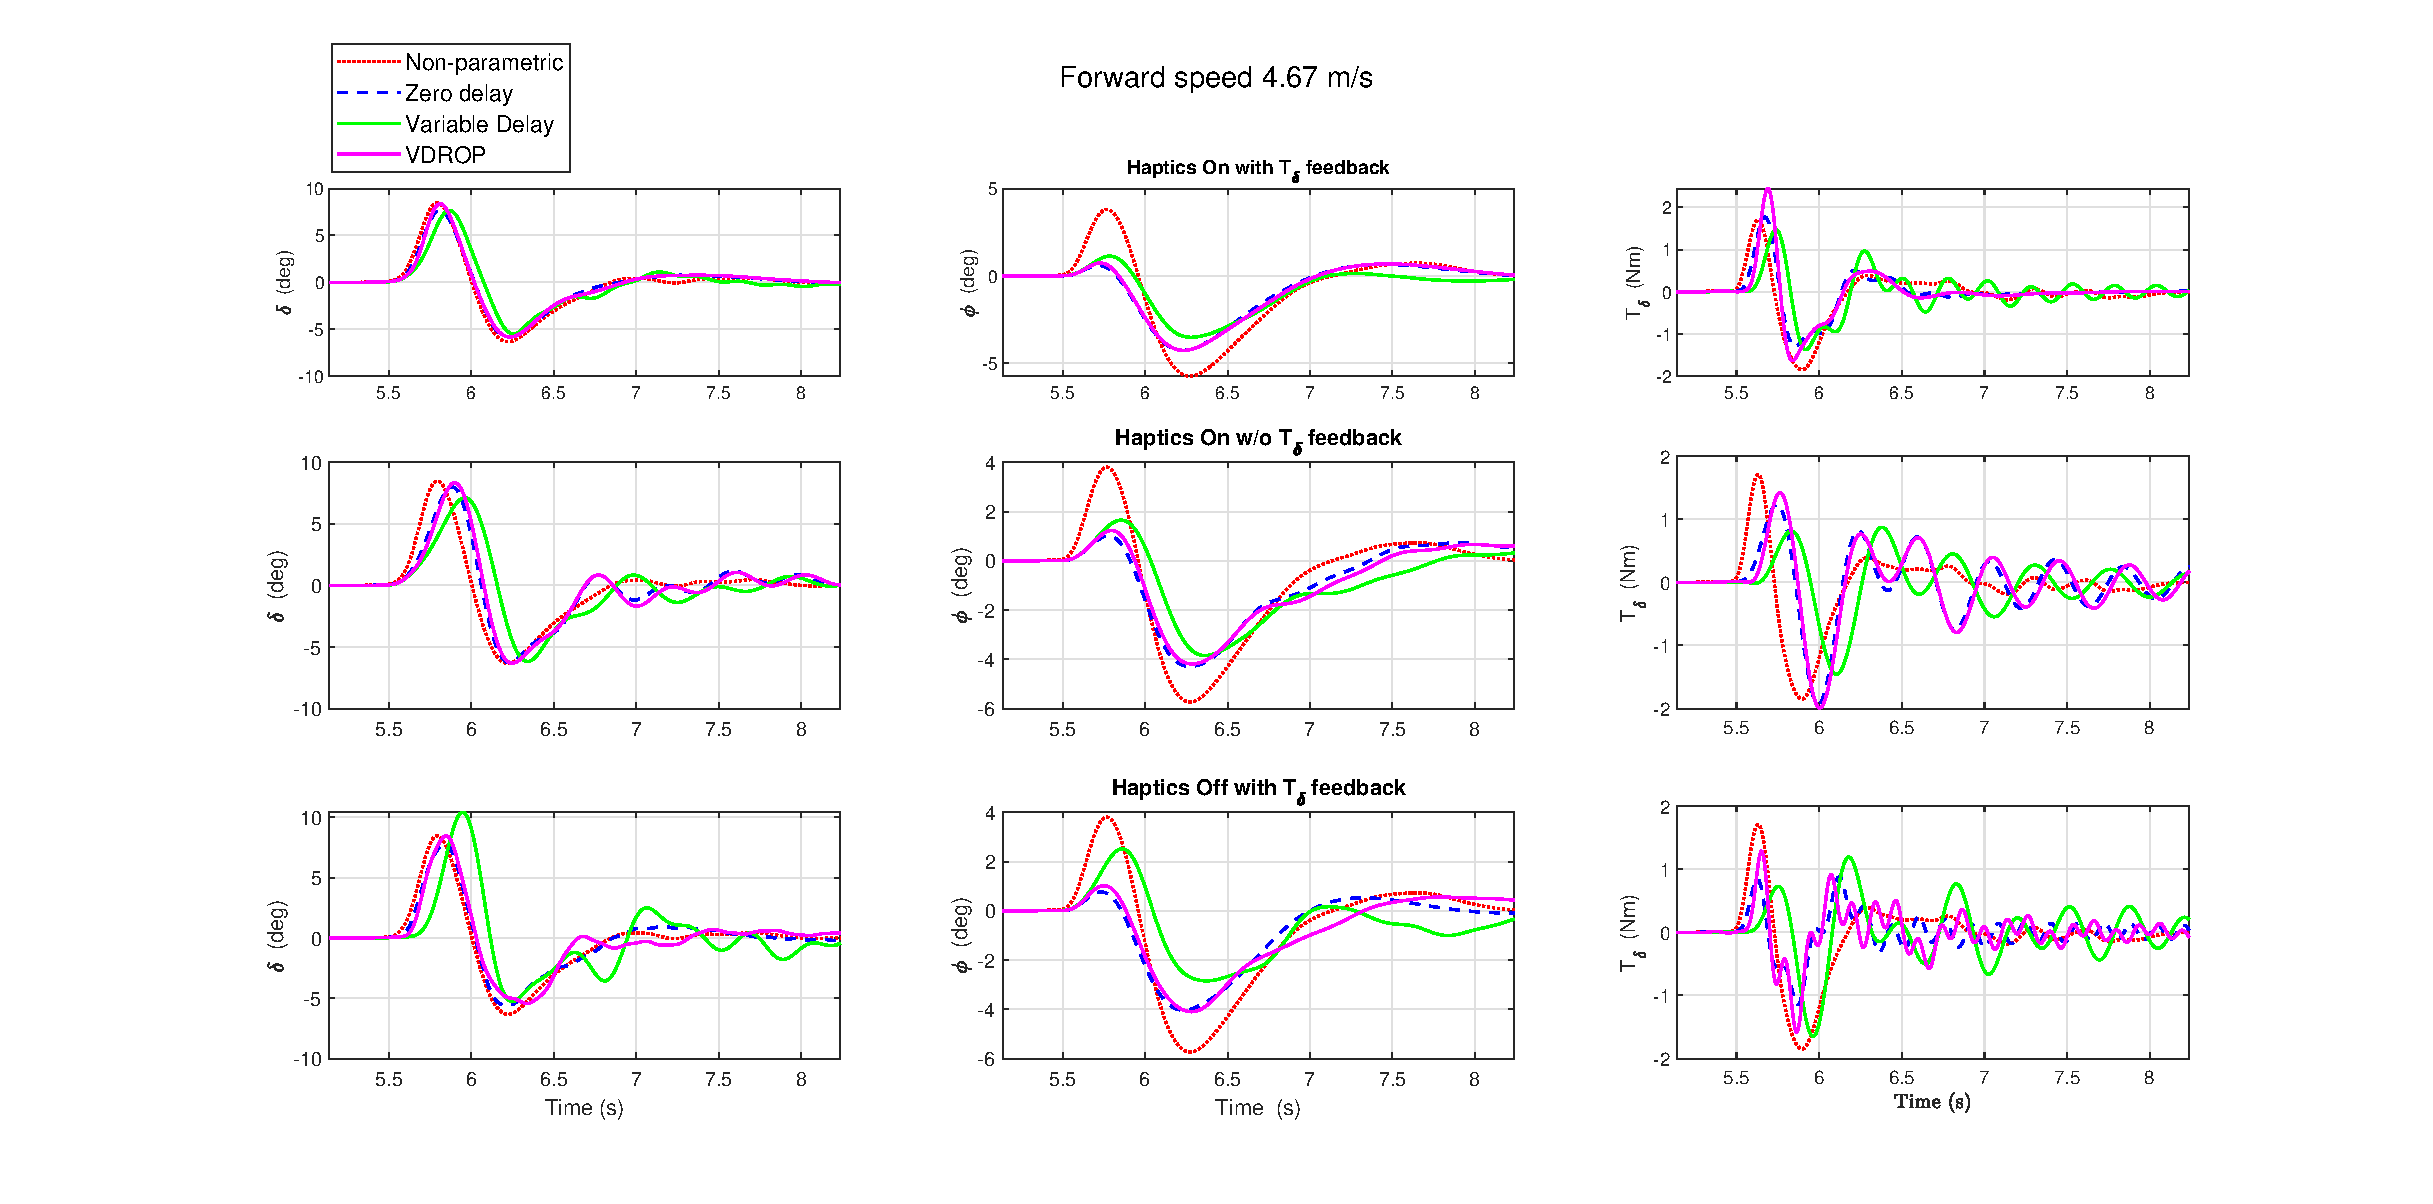
\includegraphics[width=1.2\linewidth]{images/compare_model_plots/compare_models_46.eps}}
            \caption{Comparison between the three rider models for forward speed 4.67 \si{\meter\per\second}}
            \label{fig:results_compare3}
        \end{subfigure}
        \begin{subfigure}[b]{\textwidth}
            \centering
            \makebox[\textwidth][c]{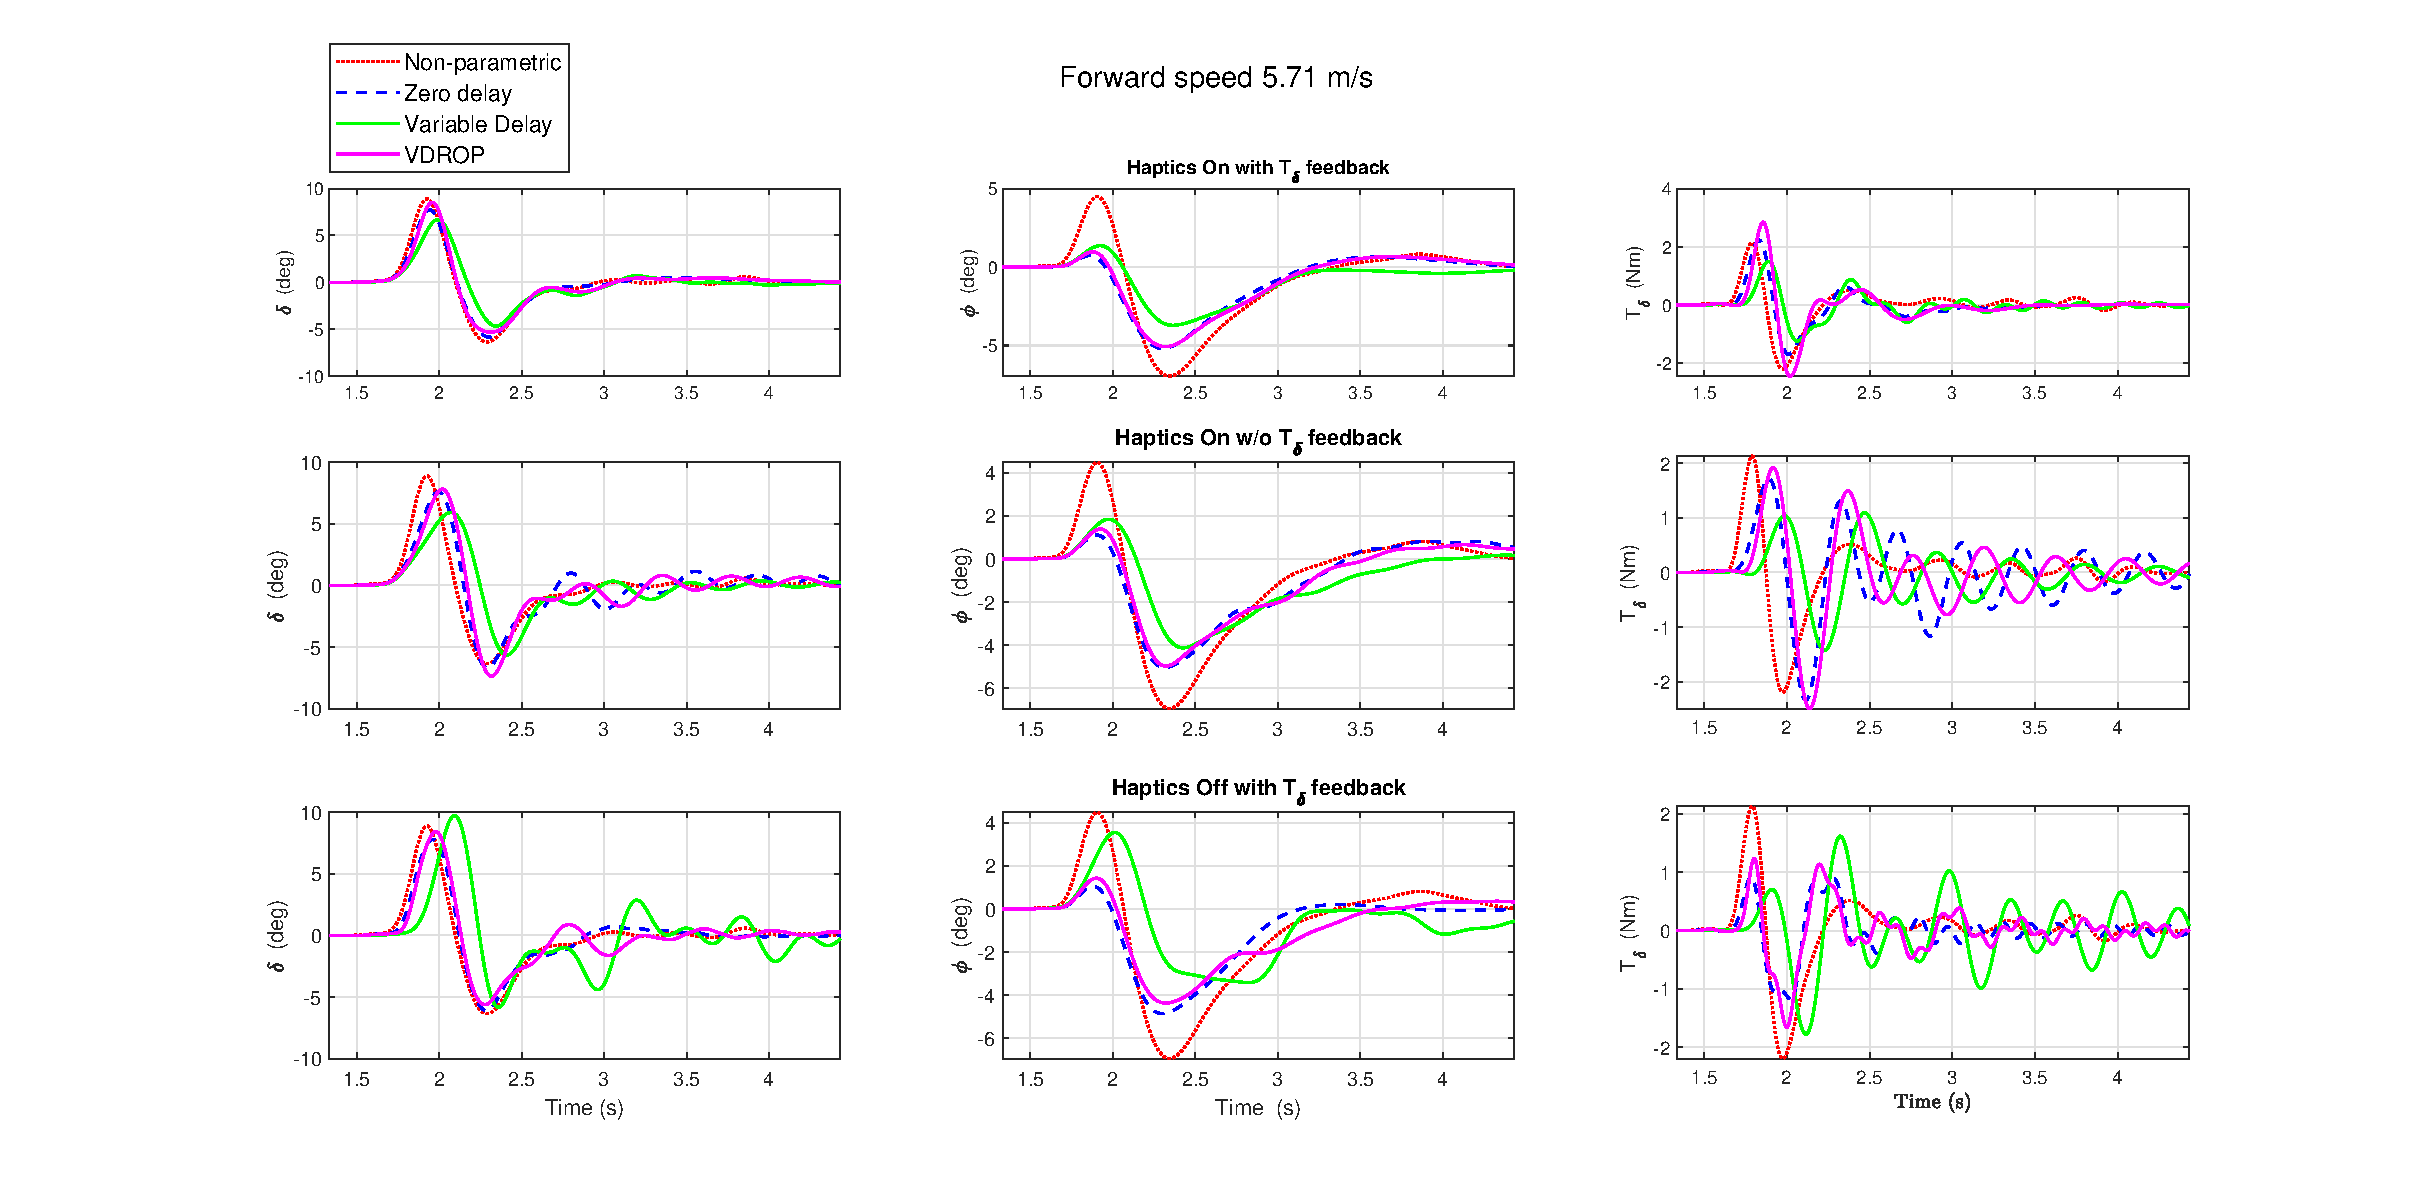
\includegraphics[width=1.2\linewidth]{images/compare_model_plots/compare_models_57.eps}}
            \caption{Comparison between the three rider models for forward speed 5.71 \si{\meter\per\second}}            
            \label{fig:results_compare4}
        \end{subfigure}
        \caption{Steering angle \ensuremath{\delta}, roll angle \ensuremath{\phi} and steering torque \ensuremath{T_\delta} compared among the three rider models implemented for all torque feedback conditions, for the two highest speed levels for the response of the median rider to the first perturbation of each run. Non-parametric output included for reference.}
        \label{fig:results_compare34}
     \end{figure}
Finally, In order to assess the effectiveness of the Reafferent Optimal Predictor, the ROP model is compared with an implementation of the prediction algorithm without the smith correction, meaning the predictor consists of just the discrete optimal predictor (see \cref{fig:delay_line}). For the comparison the gains estimated from the zero delay model are used, so as to remove any potential adaptation that might give the ROP model an advantage. The effect of the undelayed estimate using both approaches is seen in \cref{fig:predictor_compare}
\begin{figure}[!h]
    \centering
    \captionsetup{justification=centering,margin=2cm}

    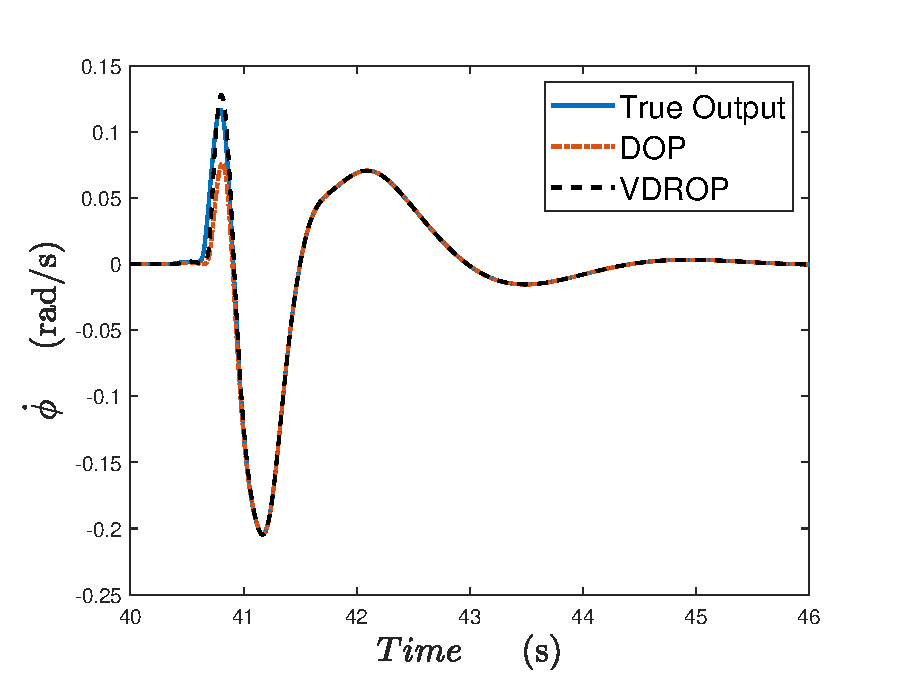
\includegraphics[width=\textwidth]{images/predictor_plots/rate_compare.eps}
    \caption{Comparison between true roll rate (red), and predicted roll rate using the reafferent optimal predictor(blue) and the discrete optimal predictor (black)}
    \label{fig:predictor_compare}
\end{figure}

From \cref{fig:predictor_compare} it is visible that the estimate of the state significantly improves due to the fact that the effect of the disturbance on the state albeit delayed is added back to the optimal prediction. Worth noting that both prediction strategies produce satisfactory results and manage to stabilize the system. However, the main advantage of  ROP is its ability to correct for internal model inaccuracies. In \cref{fig:predictor_compareA} the results of a simulation using ROP  model is compared with the results of the discrete optimal predictor but in this case internal model imperfections are introduced. This is done by replacing the perfect forward model with  the one used for the haptics off steering dynamics. The reasoning behind that is based on the assumption that the human has a reduced perception of bicycle dynamics that does not take into account the fact that roll also affects the state of the handlebar assembly. ROP manages to produce a good estimate of the state as can be seen in \cref{fig:predictor_compare1}. In \cref{fig:predictor_compare2} it is visible that ROP manages to stabilize the system while the simple optimal predictor fails.

\begin{figure}
    \centering
    \begin{subfigure}[b]{\textwidth}
        \centering
        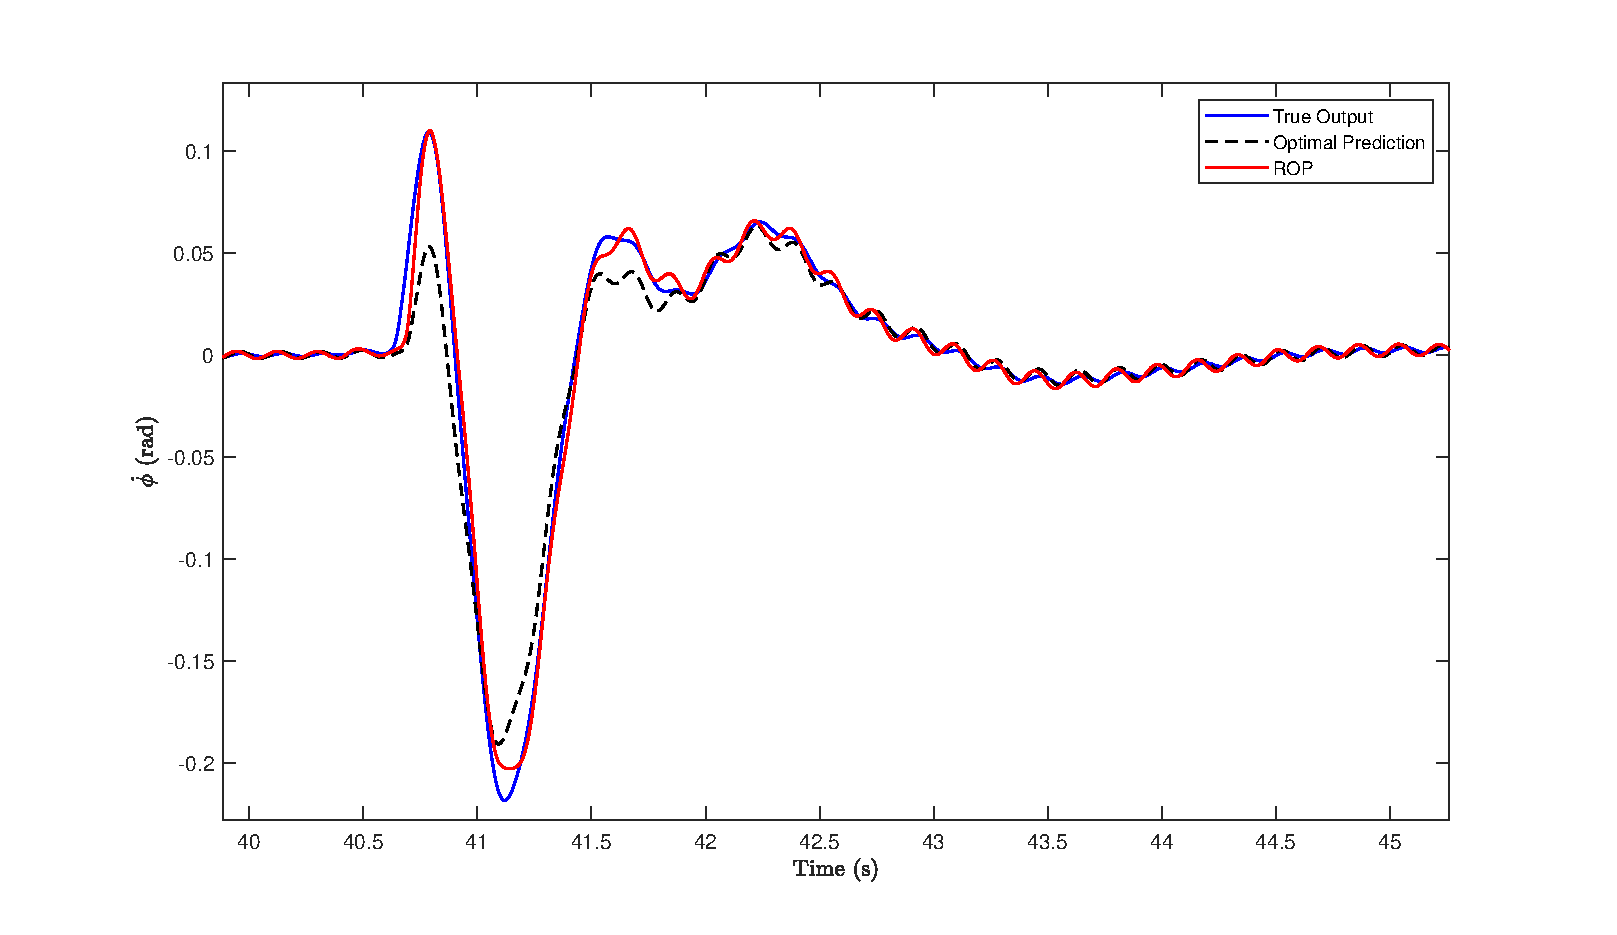
\includegraphics[width=\linewidth]{images/predictor_plots/rate_compare2.eps}
        \caption{Comparison between true roll rate (blue), and predicted roll rate using the reafferent optimal predictor(red) and the discrete optimal predictor (dotted black)}
        \label{fig:predictor_compare1}
    \end{subfigure}
    \begin{subfigure}[b]{\textwidth}
        \centering
       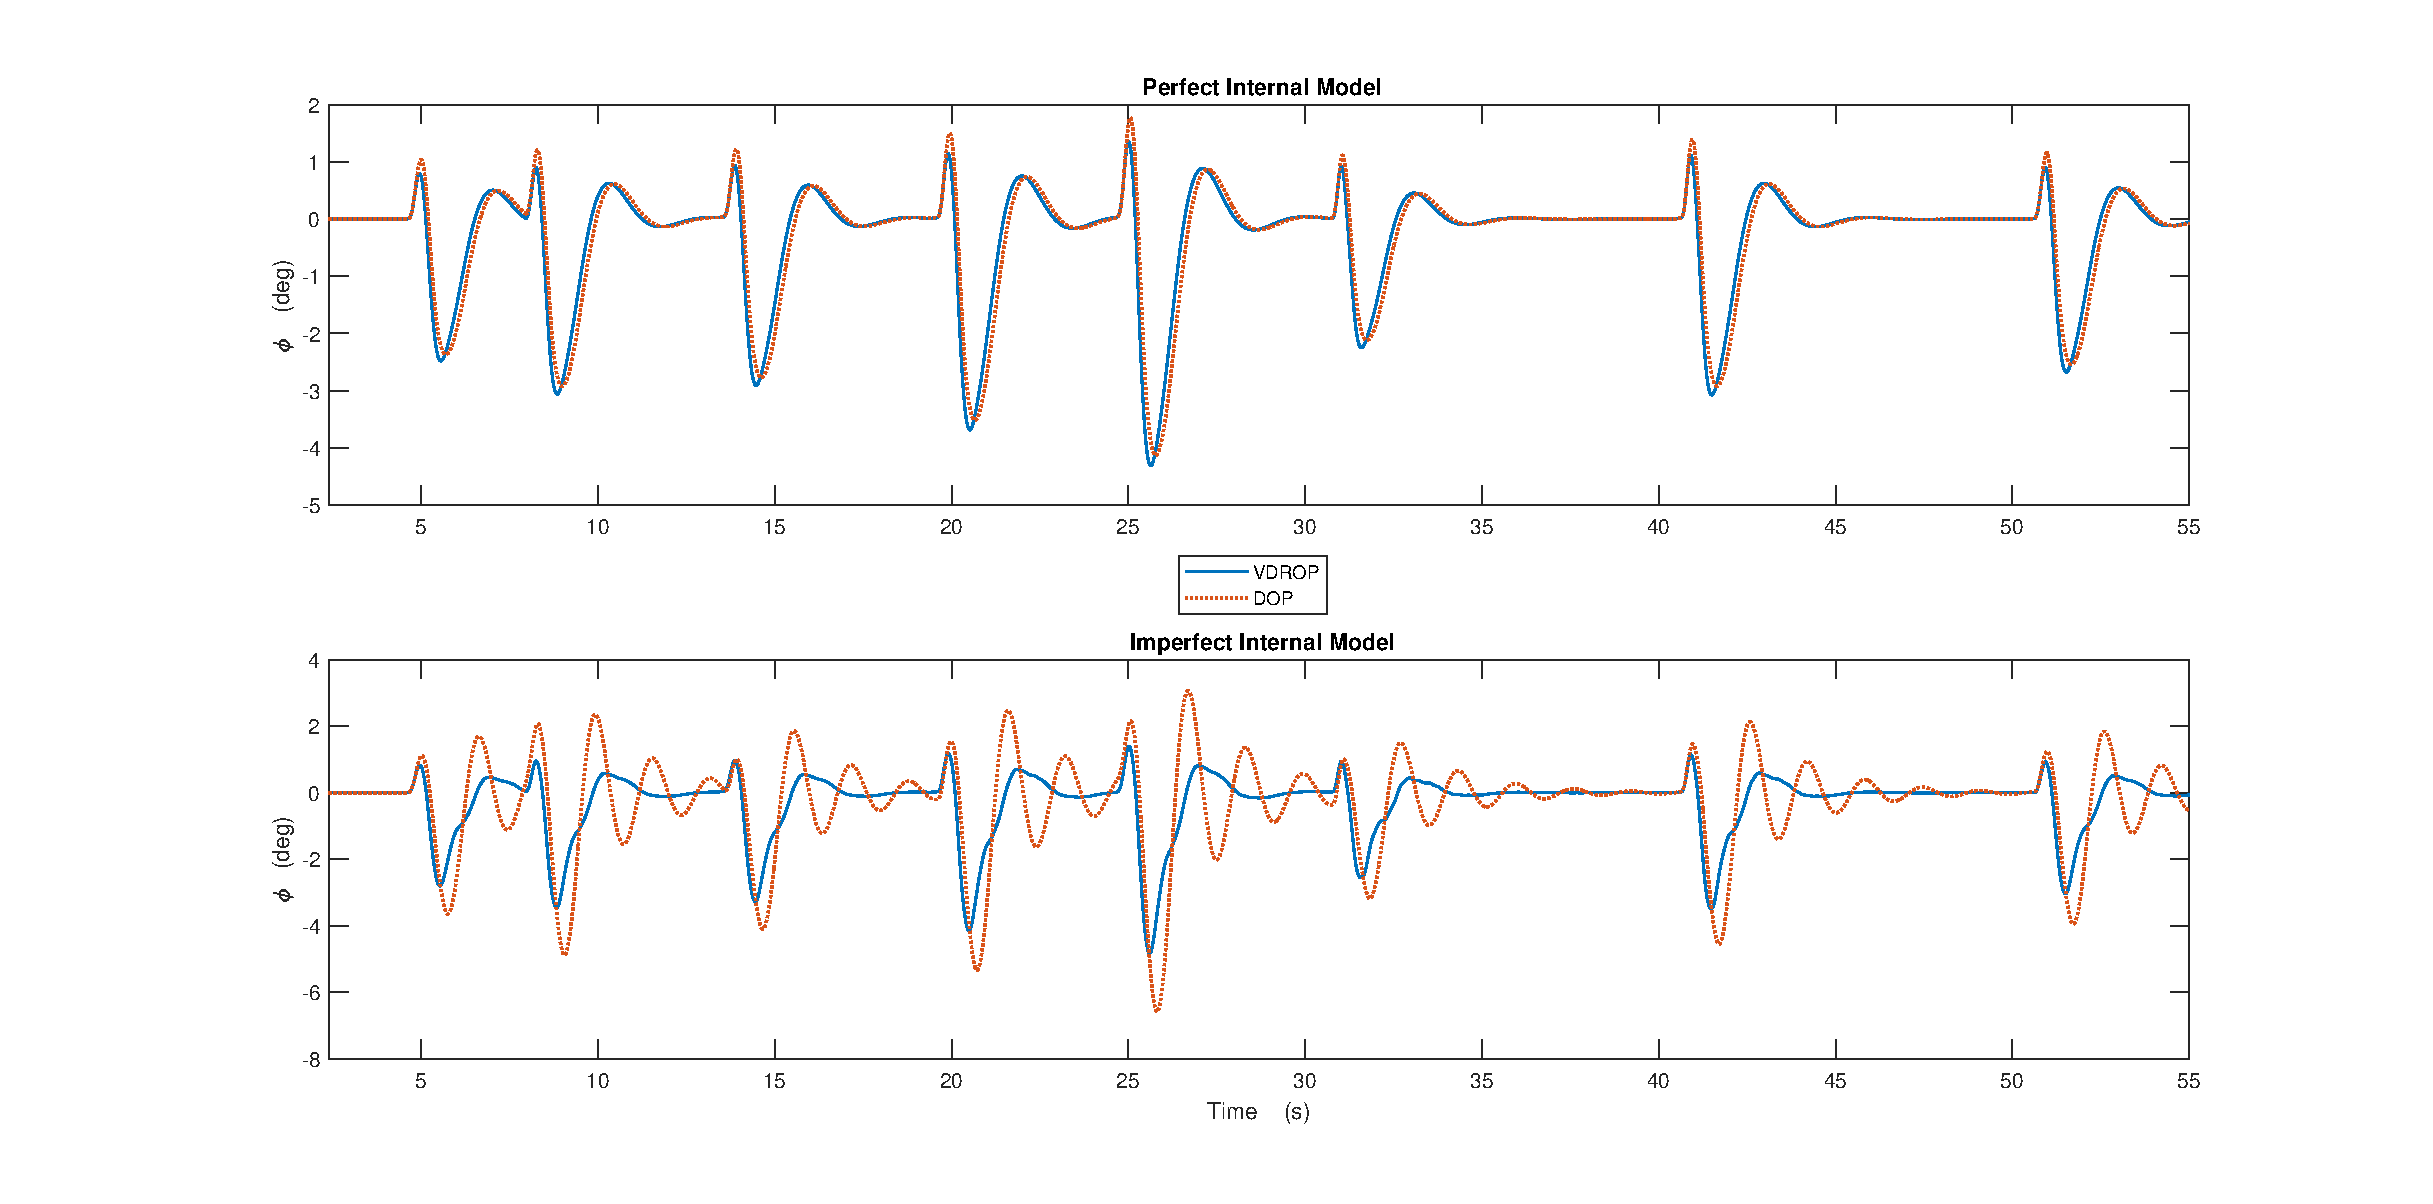
\includegraphics[width=\linewidth]{images/predictor_plots/compare_imperfect.eps}
        \caption{Steering torque and steering angle compared for a simulation using ROP and a simulation using the discrete optimal predictor.}            
        \label{fig:predictor_compare2}
    \end{subfigure}
    \caption{Results of the simulation using imperfect internal model. In (a) the state estimate of the roll rate is compared among prediction algorithms, while in (b) the steering  response to a prolong run subject to  the different prediction strategies is shown.}
    \label{fig:predictor_compareA}
 \end{figure}


     \begin{figure}
        \centering
        \begin{subfigure}[b]{\textwidth}
            \centering
            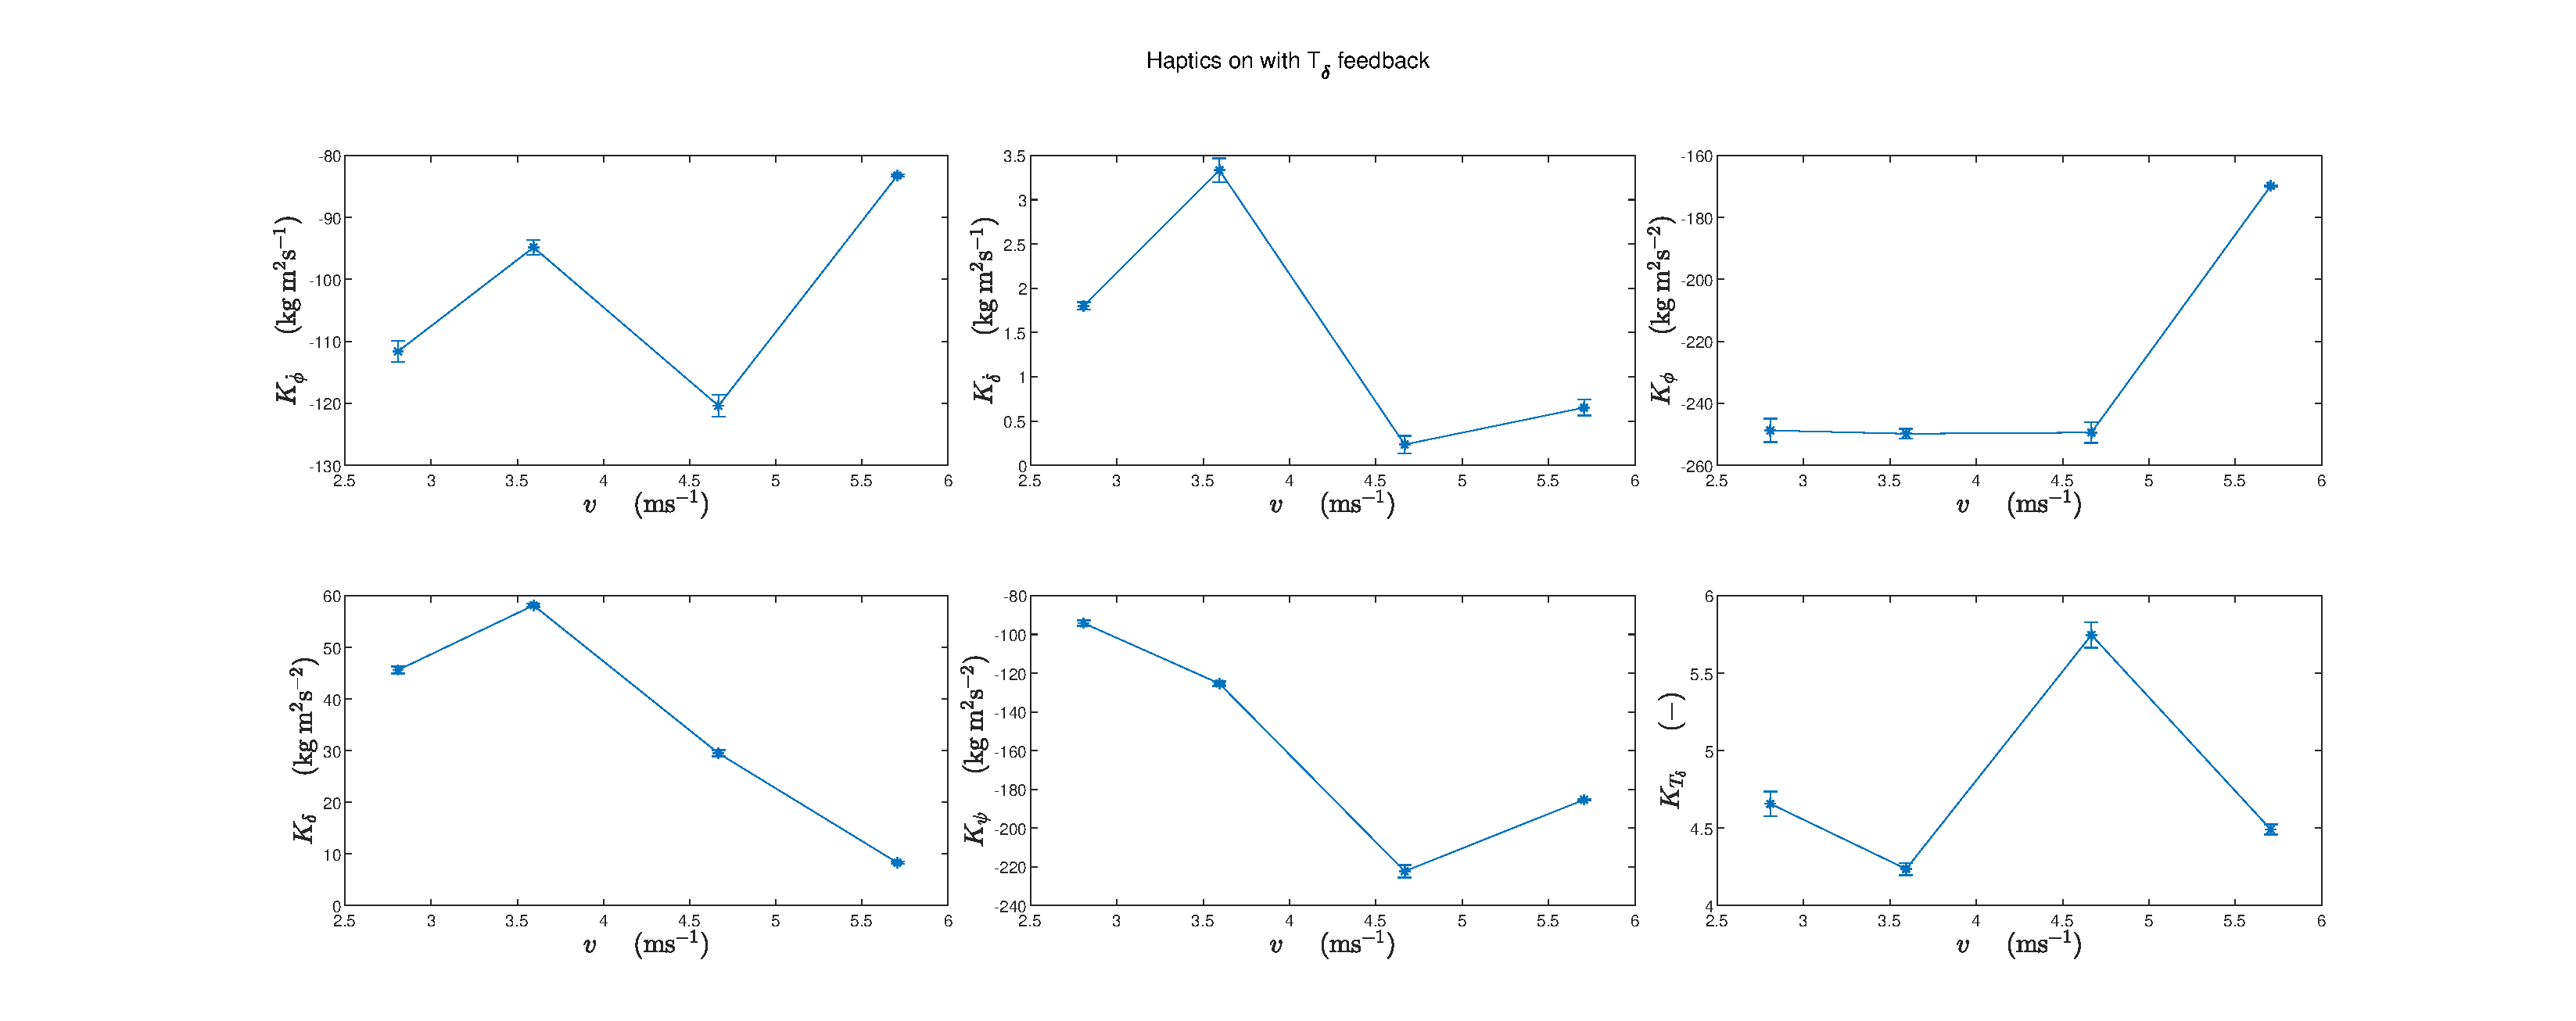
\includegraphics[width=1\linewidth]{images/gain_plots/hap_on_td_predict.eps}
            \caption{}
            \label{fig:gains_speed1}
        \end{subfigure}
        \begin{subfigure}[b]{\textwidth}
            \centering
            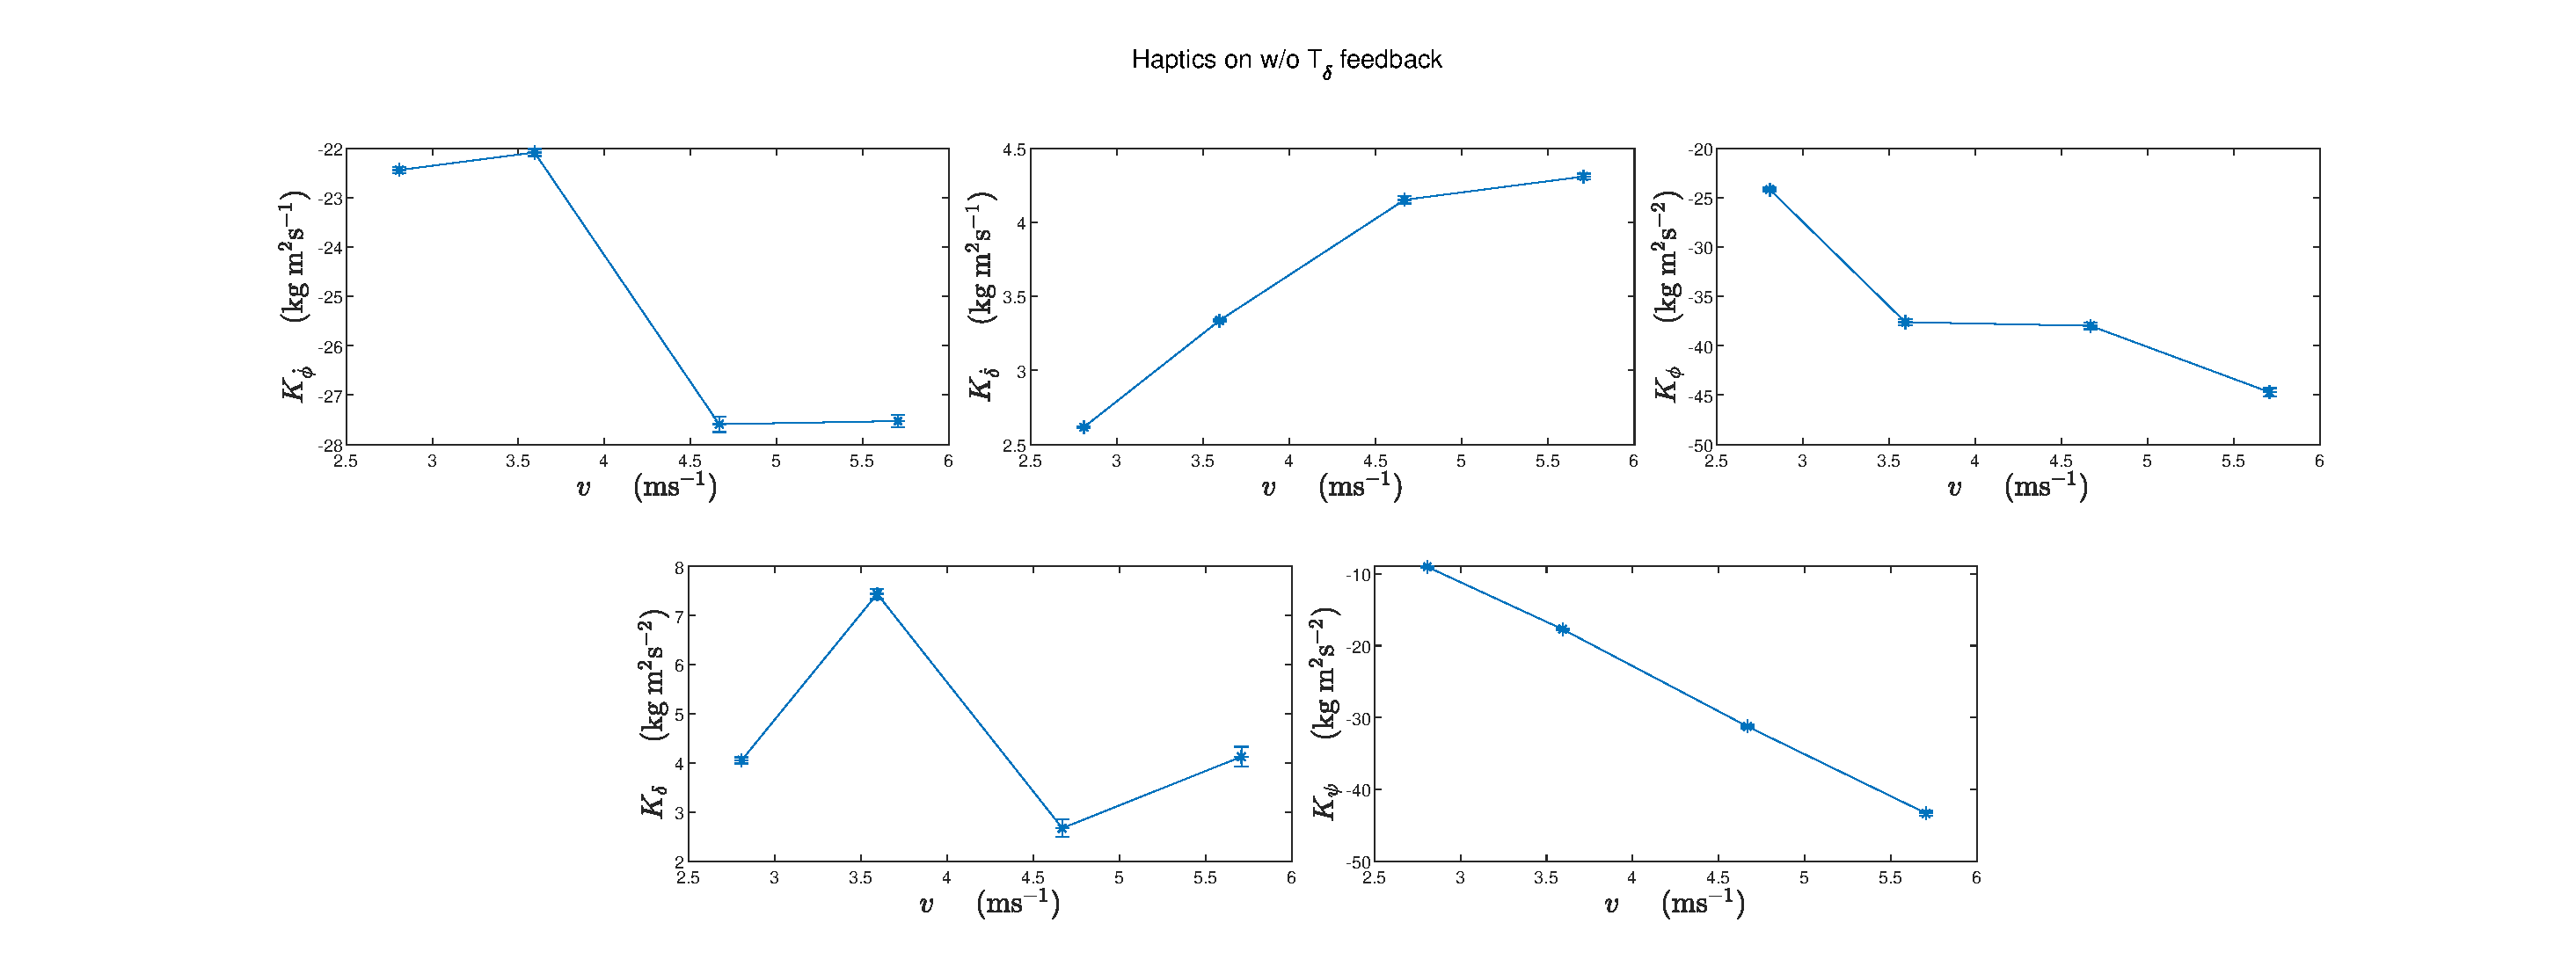
\includegraphics[width=1\linewidth]{images/gain_plots/hap_on_predict.eps}
            \caption{}            
            \label{fig:gains_speed2}
        \end{subfigure}
        \begin{subfigure}[b]{\textwidth}
            \centering
            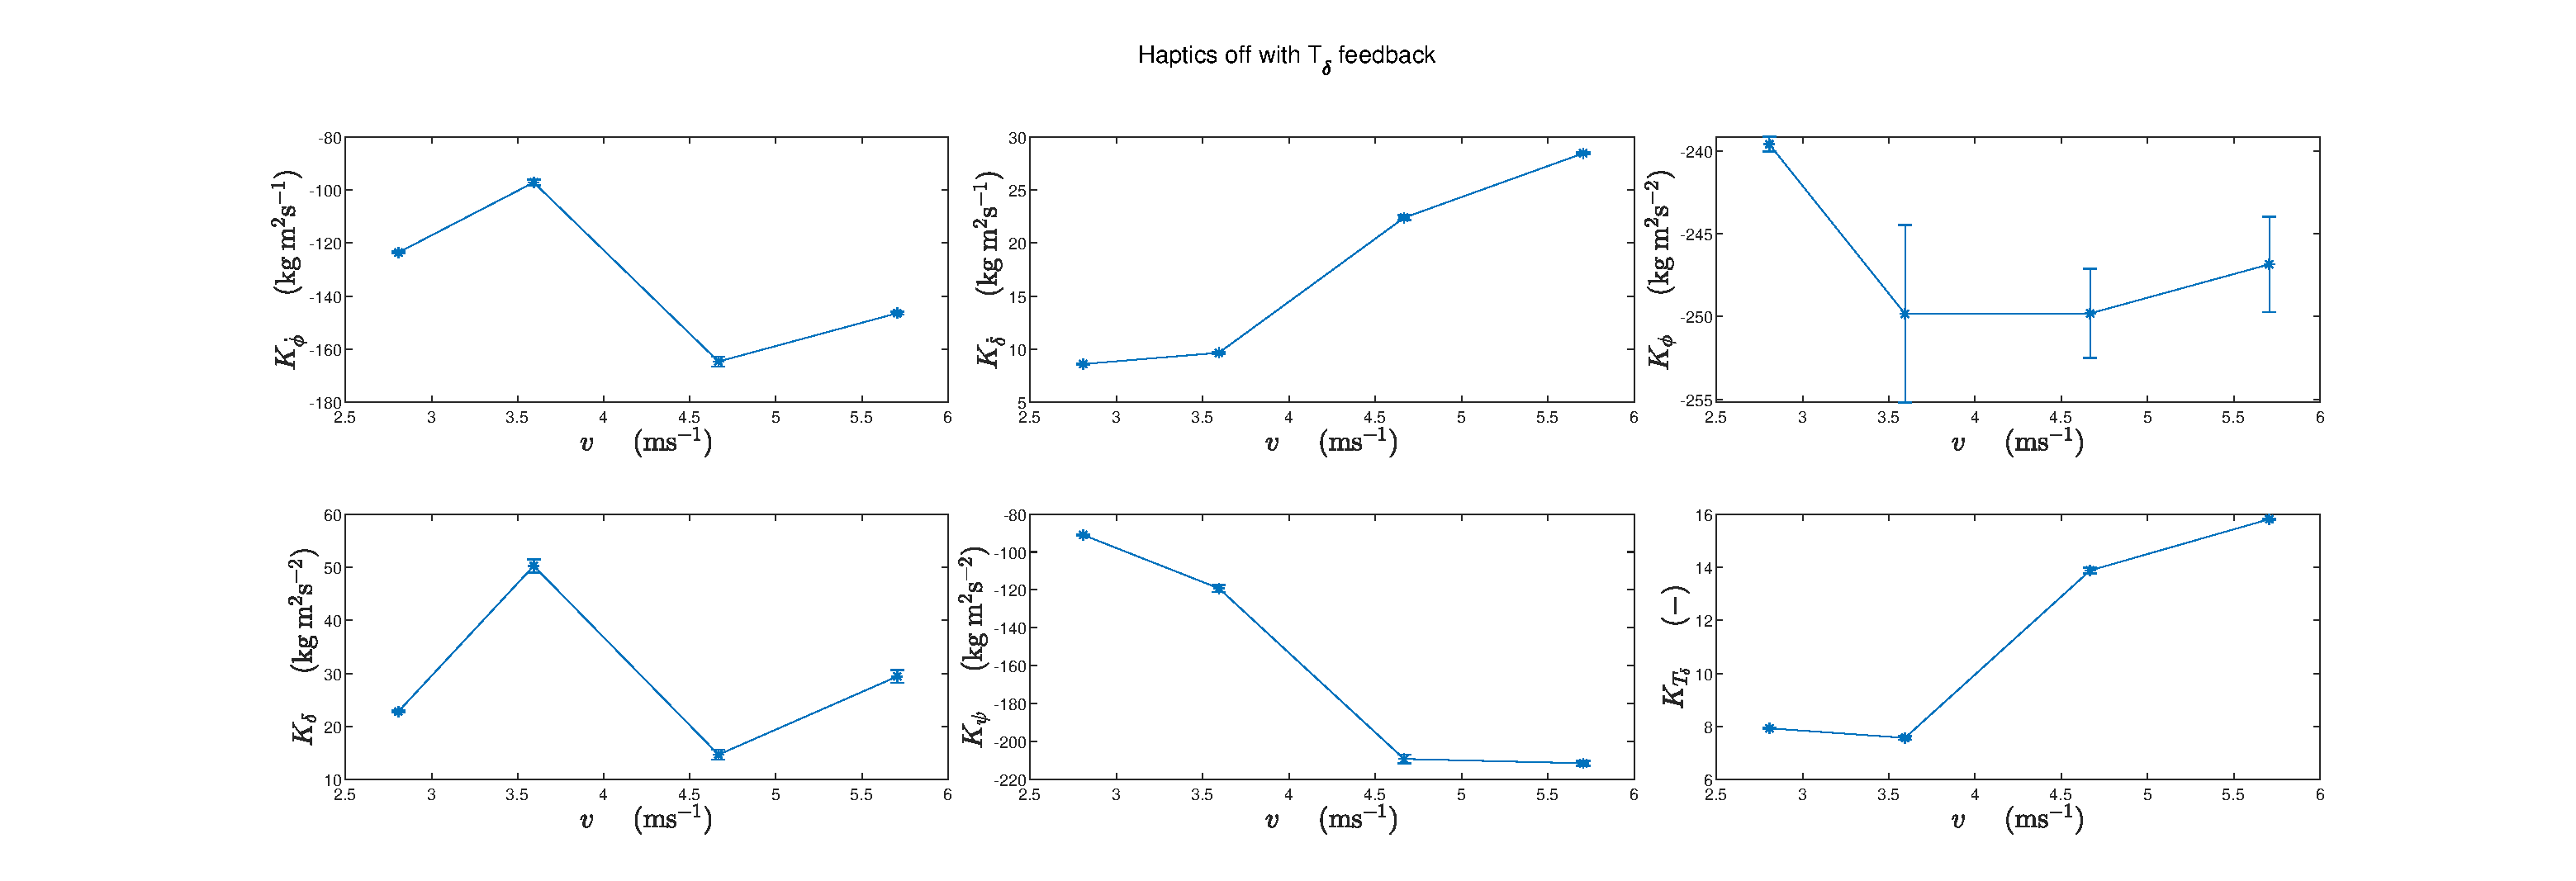
\includegraphics[width=1\linewidth]{images/gain_plots/hap_off_td_predict.eps}
            \caption{}            
            \label{fig:gains_speed3}
        \end{subfigure}
        \caption{Feedback control gains (\ensuremath{K}) as a function of forward velocity (\ensuremath{v}) for the different torque feedback levels for the median rider in the ROP Model. Error bars indicate the standard errror of the mean calculated from the covariance matrix calculated by \cref{fig:cov_mat}.}
        \label{fig:gains_speed}
     \end{figure}




\begin{table}[]
    \caption{ Results for the zero delay model as estimated for the median rider for all speed levels. Results are presented for the three conditions. Haptic on/off differentiates based on the dynamics of the bicycle model, while "with or w/o \ensuremath{T_\delta} feedback" differentiates based on the structure of the rider control model. The values of the gains are presented as well as their corresponding uncertainty level measured by the coefficient of variation \ensuremath{CV_i}. Additionally, the variance accounted for of the orientation outputs between parametric and non parametric signals is also presented. The derivative gains (\ensuremath{K_{\dot{\phi}}},\ensuremath{K_{\dot{\delta}}}) are measured in \si{\kilogram\square\meter\per\square\second} while the proportional gains (\ensuremath{K_{\phi}},\ensuremath{K_{\delta}},\ensuremath{K_{\psi}}) are measured in \si{\kilogram\square\meter\per\second}. The torque feedback gain \ensuremath{K_{T_\delta}} is dimensionless.}
    \label{tb:no_delay}
    \begin{tabular}{llcccccc}
    \hline
                                                   & Bicycle $\rightarrow$                                              & \multicolumn{4}{c}{Haptic On}                                                                                                                                                                         & \multicolumn{2}{c}{Haptic Off}                                                                    \\ \cline{2-8} 
                                                   & {\color[HTML]{333333} Rider $\;\;\;\;\rightarrow$} & \multicolumn{2}{l}{with $T_\delta$ feedback}                                                      & \multicolumn{2}{l}{w/o  $T_\delta$ feedback}                                                      & \multicolumn{2}{l}{with $T_\delta$ feedback}                                                      \\ \cline{2-8} 
                                                   &                                                                    & \multicolumn{1}{l}{}                        & \multicolumn{1}{l}{}                                & \multicolumn{1}{l}{}                        & \multicolumn{1}{l}{}                                & \multicolumn{1}{l}{}                        & \multicolumn{1}{l}{}                                \\
    \multirow{-2}{*}{Forward Speed}                &                                                                    & \multicolumn{1}{l}{\multirow{-2}{*}{Value}} & \multicolumn{1}{l}{\multirow{-2}{*}{CV ($10^{-4}$)}} & \multicolumn{1}{l}{\multirow{-2}{*}{Value}} & \multicolumn{1}{l}{\multirow{-2}{*}{CV ($10^{-4}$)}} & \multicolumn{1}{l}{\multirow{-2}{*}{Value}} & \multicolumn{1}{l}{\multirow{-2}{*}{CV ($10^{-4}$)}} \\ \hline
                                                   & $K_{\dot{\phi}} $                                                  & -77.17                                      & 114.86                                              & -22.46                                      & 29.77                                               & -115.36                                     & 213.52                                              \\
    \multirow{-2}{*}{2.8 $\si{\meter\per\second}$} & $K_{\dot{\delta}}$                                                 & 2.26                                        & 73.57                                               & 2.58                                        & 18.93                                               & 8.76                                        & 187.30                                              \\
                                                   & $K_{\phi} $                                                        & -164.88                                     & 132.25                                              & -24.50                                      & 73.14                                               & -248.24                                     & 217.05                                              \\
                                                   & $K_\delta $                                                        & 32.75                                       & 150.14                                              & 3.76                                        & 140.96                                              & 29.67                                       & 215.07                                              \\
                                                   & $K_\psi $                                                          & -63.22                                      & 133.29                                              & -9.85                                       & 53.71                                               & -93.44                                      & 223.02                                              \\
                                                   & $K_{T_\delta}$                                                     & 3.51                                        & 176.20                                              & -                                           & -                                                   & 7.53                                        & 223.83                                              \\ \cline{2-8} 
                                                   & $\mathbf{VAF}_\phi$                                                & \multicolumn{2}{c}{77.80}                                                                         & \multicolumn{2}{c}{82.79}                                                                         & \multicolumn{2}{c}{78.37}                                                                         \\
                                                   & $\mathbf{VAF}_\delta$                                              & \multicolumn{2}{c}{98.34}                                                                         & \multicolumn{2}{c}{79.19}                                                                         & \multicolumn{2}{c}{98.20}                                                                         \\
                                                   & $\mathbf{VAF}_\psi$                                                & \multicolumn{2}{c}{93.46}                                                                         & \multicolumn{2}{c}{93.51}                                                                         & \multicolumn{2}{c}{93.74}                                                                         \\
                                                   &                                                                    & \multicolumn{1}{l}{}                        & \multicolumn{1}{l}{}                                & \multicolumn{1}{l}{}                        & \multicolumn{1}{l}{}                                & \multicolumn{1}{l}{}                        & \multicolumn{1}{l}{}                                \\ \hline
                                                   & $K_{\dot{\phi}} $                                                  & -109.94                                     & 146.98                                              & -21.30                                      & 35.99                                               & -78.28                                      & 61.00                                               \\
    \multirow{-2}{*}{3.6 $\si{\meter\per\second}$} & $K_{\dot{\delta}}$                                                 & 8.22                                        & 139.00                                              & 3.30                                        & 24.78                                               & 9.09                                        & 51.11                                               \\
                                                   & $K_{\phi} $                                                        & -248.47                                     & 147.39                                              & -34.64                                      & 71.54                                               & -229.14                                     & 84.40                                               \\
                                                   & $K_\delta $                                                        & 50.78                                       & 147.72                                              & 6.48                                        & 130.57                                              & 53.16                                       & 92.96                                               \\
                                                   & $K_\psi $                                                          & -132.13                                     & 152.08                                              & -17.74                                      & 61.92                                               & -103.75                                     & 74.49                                               \\
                                                   & $K_{T_\delta}$                                                     & 4.52                                        & 167.24                                              & -                                           & -                                                   & 6.89                                        & 64.17                                               \\ \cline{2-8} 
                                                   & $\mathbf{VAF}_\phi$                                                & \multicolumn{2}{c}{79.92}                                                                         & \multicolumn{2}{c}{85.93}                                                                         & \multicolumn{2}{c}{80.89}                                                                         \\
                                                   & $\mathbf{VAF}_\delta$                                              & \multicolumn{2}{c}{98.83}                                                                         & \multicolumn{2}{c}{86.40}                                                                         & \multicolumn{2}{c}{97.08}                                                                         \\
                                                   & $\mathbf{VAF}_\psi$                                                & \multicolumn{2}{c}{95.33}                                                                         & \multicolumn{2}{c}{97.95}                                                                         & \multicolumn{2}{c}{95.15}                                                                         \\
                                                   &                                                                    & \multicolumn{1}{l}{}                        & \multicolumn{1}{l}{}                                & \multicolumn{1}{l}{}                        & \multicolumn{1}{l}{}                                & \multicolumn{1}{l}{}                        & \multicolumn{1}{l}{}                                \\ \hline
                                                   & $K_{\dot{\phi}} $                                                  & -92.50                                      & 117.34                                              & -27.29                                      & 46.40                                               & -102.63                                     & 40.87                                               \\
    \multirow{-2}{*}{4.7 $\si{\meter\per\second}$} & $K_{\dot{\delta}}$                                                 & 4.81                                        & 183.05                                              & 4.25                                        & 41.56                                               & 11.24                                       & 28.38                                               \\
                                                   & $K_{\phi} $                                                        & -183.03                                     & 135.64                                              & -38.17                                      & 76.43                                               & -249.74                                     & 74.10                                               \\
                                                   & $K_\delta $                                                        & 22.57                                       & 237.51                                              & 2.65                                        & 591.87                                              & 63.36                                       & 88.33                                               \\
                                                   & $K_\psi $                                                          & -165.42                                     & 126.89                                              & -33.78                                      & 63.74                                               & -188.67                                     & 58.81                                               \\
                                                   & $K_{T_\delta}$                                                     & 3.42                                        & 174.23                                              & -                                           & -                                                   & 8.98                                        & 13.88                                               \\ \cline{2-8} 
                                                   & $\mathbf{VAF}_\phi$                                                & \multicolumn{2}{c}{77.03}                                                                         & \multicolumn{2}{c}{83.06}                                                                         & \multicolumn{2}{c}{78.60}                                                                         \\
                                                   & $\mathbf{VAF}_\delta$                                              & \multicolumn{2}{c}{97.57}                                                                         & \multicolumn{2}{c}{80.27}                                                                         & \multicolumn{2}{c}{95.57}                                                                         \\
                                                   & $\mathbf{VAF}_\psi$                                                & \multicolumn{2}{c}{91.41}                                                                         & \multicolumn{2}{c}{97.03}                                                                         & \multicolumn{2}{c}{92.48}                                                                         \\
                                                   &                                                                    & \multicolumn{1}{l}{}                        & \multicolumn{1}{l}{}                                & \multicolumn{1}{l}{}                        & \multicolumn{1}{l}{}                                & \multicolumn{1}{l}{}                        & \multicolumn{1}{l}{}                                \\ \hline
                                                   & $K_{\dot{\phi}} $                                                  & -83.90                                      & 117.61                                              & -31.12                                      & 43.99                                               & -76.30                                      & 47.12                                               \\
    \multirow{-2}{*}{5.7 $\si{\meter\per\second}$} & $K_{\dot{\delta}}$                                                 & 5.83                                        & 142.87                                              & 5.58                                        & 40.62                                               & 10.91                                       & 30.23                                               \\
                                                   & $K_{\phi} $                                                        & -166.08                                     & 127.89                                              & -43.64                                      & 67.14                                               & -208.33                                     & 83.09                                               \\
                                                   & $K_\delta $                                                        & 14.85                                       & 98.10                                               & 1.14                                        & 1836.39                                             & 79.44                                       & 75.47                                               \\
                                                   & $K_\psi $                                                          & -186.77                                     & 128.56                                              & -49.82                                      & 52.31                                               & -176.96                                     & 69.82                                               \\
                                                   & $K_{T_\delta}$                                                     & 3.24                                        & 185.07                                              & -                                           & -                                                   & 8.45                                        & 29.67                                               \\ \cline{2-8} 
                                                   & $\mathbf{VAF}_\phi$                                                & \multicolumn{2}{c}{79.17}                                                                         & \multicolumn{2}{c}{84.03}                                                                         & \multicolumn{2}{c}{80.30}                                                                         \\
                                                   & $\mathbf{VAF}_\delta$                                              & \multicolumn{2}{c}{97.51}                                                                         & \multicolumn{2}{c}{84.09}                                                                         & \multicolumn{2}{c}{94.71}                                                                         \\
                                                   & $\mathbf{VAF}_\psi$                                                & \multicolumn{2}{c}{90.97}                                                                         & \multicolumn{2}{c}{96.41}                                                                         & \multicolumn{2}{c}{91.56}                                                                        
    \end{tabular}
    \end{table}

\begin{table}[]
    \caption{ Results for the variable delay model as estimated for the median rider for all speed levels. Results are presented for the three conditions. Haptic on/off differentiates based on the dynamics of the bicycle model, while "with or w/o \ensuremath{T_\delta} feedback" differentiates based on the structure of the rider control model. The values of the gains are presented as well as their corresponding uncertainty level measured by the coefficient of variation \ensuremath{CV_i}. Additionally, the variance accounted for of the orientation outputs between parametric and non parametric signals is also presented. The derivative gains (\ensuremath{K_{\dot{\phi}}},\ensuremath{K_{\dot{\delta}}}) are measured in \si{\kilogram\square\meter\per\square\second} while the proportional gains (\ensuremath{K_{\phi}},\ensuremath{K_{\delta}},\ensuremath{K_{\psi}}) are measured in \si{\kilogram\square\meter\per\second}. The torque feedback gain \ensuremath{K_{T_\delta}} is dimensionless.}
    \label{tb:variable}
    \begin{tabular}{llcccccc}
    \hline
                                                   & Bicycle $\rightarrow$                                  & \multicolumn{4}{c}{Haptic On}                                                                                                                                                                           & \multicolumn{2}{c}{Haptic Off}                                                                     \\ \cline{2-8} 
                                                   & {\color[HTML]{333333} Rider $\;\;\;\;\rightarrow$} & \multicolumn{2}{l}{with $T_\delta$ feedback}                                                       & \multicolumn{2}{l}{w/o  $T_\delta$ feedback}                                                       & \multicolumn{2}{l}{with $T_\delta$ feedback}                                                       \\ \cline{2-8} 
                                                   &                                                        & \multicolumn{1}{l}{}                        & \multicolumn{1}{l}{}                                 & \multicolumn{1}{l}{}                        & \multicolumn{1}{l}{}                                 & \multicolumn{1}{l}{}                        & \multicolumn{1}{l}{}                                 \\
    \multirow{-2}{*}{Forward Speed}                &                                                        & \multicolumn{1}{l}{\multirow{-2}{*}{Value}} & \multicolumn{1}{l}{\multirow{-2}{*}{CV ($10^{-4}$)}} & \multicolumn{1}{l}{\multirow{-2}{*}{Value}} & \multicolumn{1}{l}{\multirow{-2}{*}{CV ($10^{-4}$)}} & \multicolumn{1}{l}{\multirow{-2}{*}{Value}} & \multicolumn{1}{l}{\multirow{-2}{*}{CV ($10^{-4}$)}} \\ \hline
                                                   & $K_{\dot{\phi}} $                                      & -68.53                                      & 38.72                                                & -14.93                                      & 37.52                                                & -28.19                                      & 35.15                                                \\
    \multirow{-2}{*}{2.8 $\si{\meter\per\second}$} & $K_{\dot{\delta}}$                                     & 2.09                                        & 110.32                                               & 2.30                                        & 32.17                                                & 2.65                                        & 13.18                                                \\
                                                   & $K_{\phi} $                                            & -146.29                                     & 72.07                                                & -16.98                                      & 92.51                                                & -79.20                                      & 78.41                                                \\
                                                   & $K_\delta $                                            & 22.18                                       & 95.38                                                & 4.62                                        & 103.75                                               & 10.51                                       & 93.36                                                \\
                                                   & $K_\psi $                                              & -40.34                                      & 56.18                                                & -3.78                                       & 116.84                                               & -14.53                                      & 67.08                                                \\
                                                   & $K_{T_\delta}$                                         & 3.52                                        & 64.80                                                & -                                           & -                                                    & 2.59                                        & 29.48                                                \\ \cline{2-8} 
                                                   & $\mathbf{VAF}_\phi$                                    & \multicolumn{2}{c}{81.15}                                                                          & \multicolumn{2}{c}{69.61}                                                                          & \multicolumn{2}{c}{80.01}                                                                          \\
                                                   & $\mathbf{VAF}_\delta$                                  & \multicolumn{2}{c}{93.43}                                                                          & \multicolumn{2}{c}{23.34}                                                                          & \multicolumn{2}{c}{66.84}                                                                          \\
                                                   & $\mathbf{VAF}_\psi$                                    & \multicolumn{2}{c}{93.78}                                                                          & \multicolumn{2}{c}{69.67}                                                                          & \multicolumn{2}{c}{83.30}                                                                          \\
                                                   &                                                        & \multicolumn{1}{l}{}                        & \multicolumn{1}{l}{}                                 & \multicolumn{1}{l}{}                        & \multicolumn{1}{l}{}                                 & \multicolumn{1}{l}{}                        & \multicolumn{1}{l}{}                                 \\ \hline
                                                   & $K_{\dot{\phi}} $                                      & -51.02                                      & 56.62                                                & -15.40                                      & 55.90                                                & -21.25                                      & 51.31                                                \\
    \multirow{-2}{*}{3.6 $\si{\meter\per\second}$} & $K_{\dot{\delta}}$                                     & 2.50                                        & 170.45                                               & 2.81                                        & 50.20                                                & 2.79                                        & 17.72                                                \\
                                                   & $K_{\phi} $                                            & -120.51                                     & 85.28                                                & -22.82                                      & 102.83                                               & -76.41                                      & 90.89                                                \\
                                                   & $K_\delta $                                            & 16.58                                       & 153.27                                               & 3.94                                        & 243.76                                               & 17.14                                       & 84.92                                                \\
                                                   & $K_\psi $                                              & -43.06                                      & 79.41                                                & -7.37                                       & 147.32                                               & -13.30                                      & 103.52                                               \\
                                                   & $K_{T_\delta}$                                         & 3.42                                        & 62.79                                                & -                                           & -                                                    & 3.09                                        & 21.20                                                \\ \cline{2-8} 
                                                   & $\mathbf{VAF}_\phi$                                    & \multicolumn{2}{c}{82.85}                                                                          & \multicolumn{2}{c}{79.48}                                                                          & \multicolumn{2}{c}{73.14}                                                                          \\
                                                   & $\mathbf{VAF}_\delta$                                  & \multicolumn{2}{c}{91.63}                                                                          & \multicolumn{2}{c}{53.29}                                                                          & \multicolumn{2}{c}{52.83}                                                                          \\
                                                   & $\mathbf{VAF}_\psi$                                    & \multicolumn{2}{c}{95.10}                                                                          & \multicolumn{2}{c}{84.88}                                                                          & \multicolumn{2}{c}{71.58}                                                                          \\
                                                   &                                                        & \multicolumn{1}{l}{}                        & \multicolumn{1}{l}{}                                 & \multicolumn{1}{l}{}                        & \multicolumn{1}{l}{}                                 & \multicolumn{1}{l}{}                        & \multicolumn{1}{l}{}                                 \\ \hline
                                                   & $K_{\dot{\phi}} $                                      & -51.78                                      & 64.60                                                & -19.26                                      & 349.70                                               & -14.88                                      & 55.92                                                \\
    \multirow{-2}{*}{4.7 $\si{\meter\per\second}$} & $K_{\dot{\delta}}$                                     & 2.75                                        & 160.68                                               & 4.42                                        & 438.96                                               & 3.04                                        & 20.62                                                \\
                                                   & $K_{\phi} $                                            & -136.22                                     & 105.15                                               & -27.02                                      & 111.78                                               & -48.91                                      & 115.90                                               \\
                                                   & $K_\delta $                                            & 3.21                                        & 1156.00                                              & 0.01                                        & 492609.67                                            & 16.01                                       & 99.26                                                \\
                                                   & $K_\psi $                                              & -64.43                                      & 87.60                                                & -14.29                                      & 412.99                                               & -10.82                                      & 119.48                                               \\
                                                   & $K_{T_\delta}$                                         & 3.70                                        & 63.91                                                & -                                           & -                                                    & 2.61                                        & 30.62                                                \\ \cline{2-8} 
                                                   & $\mathbf{VAF}_\phi$                                    & \multicolumn{2}{c}{77.86}                                                                          & \multicolumn{2}{c}{71.14}                                                                          & \multicolumn{2}{c}{63.73}                                                                          \\
                                                   & $\mathbf{VAF}_\delta$                                  & \multicolumn{2}{c}{81.63}                                                                          & \multicolumn{2}{c}{36.19}                                                                          & \multicolumn{2}{c}{15.61}                                                                          \\
                                                   & $\mathbf{VAF}_\psi$                                    & \multicolumn{2}{c}{90.32}                                                                          & \multicolumn{2}{c}{80.57}                                                                          & \multicolumn{2}{c}{55.71}                                                                          \\
                                                   &                                                        & \multicolumn{1}{l}{}                        & \multicolumn{1}{l}{}                                 & \multicolumn{1}{l}{}                        & \multicolumn{1}{l}{}                                 & \multicolumn{1}{l}{}                        & \multicolumn{1}{l}{}                                 \\ \hline
                                                   & $K_{\dot{\phi}} $                                      & -38.58                                      & 136.91                                               & -19.65                                      & 110.85                                               & -10.10                                      & 62.29                                                \\
    \multirow{-2}{*}{5.7 $\si{\meter\per\second}$} & $K_{\dot{\delta}}$                                     & 1.13                                        & 2085.75                                              & 5.42                                        & 128.32                                               & 3.08                                        & 21.38                                                \\
                                                   & $K_{\phi} $                                            & -120.59                                     & 120.57                                               & -33.34                                      & 117.63                                               & -30.95                                      & 133.76                                               \\
                                                   & $K_\delta $                                            & 0.00                                        & 3969013.40                                           & 0.01                                        & 280859.33                                            & 18.46                                       & 79.69                                                \\
                                                   & $K_\psi $                                              & -60.65                                      & 95.03                                                & -19.20                                      & 183.00                                               & -8.17                                       & 131.56                                               \\
                                                   & $K_{T_\delta}$                                         & 4.27                                        & 191.50                                               & -                                           & -                                                    & 2.58                                        & 26.58                                                \\ \cline{2-8} 
                                                   & $\mathbf{VAF}_\phi$                                    & \multicolumn{2}{c}{73.65}                                                                          & \multicolumn{2}{c}{70.08}                                                                          & \multicolumn{2}{c}{49.58}                                                                          \\
                                                   & $\mathbf{VAF}_\delta$                                  & \multicolumn{2}{c}{77.99}                                                                          & \multicolumn{2}{c}{40.64}                                                                          & \multicolumn{2}{c}{-}                                                                              \\
                                                   & $\mathbf{VAF}_\psi$                                    & \multicolumn{2}{c}{84.32}                                                                          & \multicolumn{2}{c}{79.50}                                                                          & \multicolumn{2}{c}{39.90}                                                                         
    \end{tabular}
    \end{table}

\begin{table}[]
    \caption{ Results for the ROP model as estimated for the median rider for all speed levels. Results are presented for the three conditions. Haptic on/off differentiates based on the dynamics of the bicycle model, while "with or w/o \ensuremath{T_\delta} feedback" differentiates based on the structure of the rider control model. The values of the gains are presented as well as their corresponding uncertainty level measured by the coefficient of variation \ensuremath{CV_i}. Additionally, the variance accounted for of the orientation outputs between parametric and non parametric signals is also presented. The derivative gains (\ensuremath{K_{\dot{\phi}}},\ensuremath{K_{\dot{\delta}}}) are measured in \si{\kilogram\square\meter\per\square\second} while the proportional gains (\ensuremath{K_{\phi}},\ensuremath{K_{\delta}},\ensuremath{K_{\psi}}) are measured in \si{\kilogram\square\meter\per\second}. The torque feedback gain \ensuremath{K_{T_\delta}} is dimensionless.}
    \label{tb:predict}
    \begin{tabular}{llcccccc}
    \hline
                                                   & Bicycle $\rightarrow$                                  & \multicolumn{4}{c}{Haptics On}                                                                                                                                                                          & \multicolumn{2}{c}{Haptics Off}                                                                    \\ \cline{2-8} 
                                                   & {\color[HTML]{333333} Rider $\;\;\;\;\rightarrow$} & \multicolumn{2}{l}{with $T_\delta$ feedback}                                                       & \multicolumn{2}{l}{w/o  $T_\delta$ feedback}                                                       & \multicolumn{2}{l}{with $T_\delta$ feedback}                                                       \\ \cline{2-8} 
                                                   &                                                        & \multicolumn{1}{l}{}                        & \multicolumn{1}{l}{}                                 & \multicolumn{1}{l}{}                        & \multicolumn{1}{l}{}                                 & \multicolumn{1}{l}{}                        & \multicolumn{1}{l}{}                                 \\
    \multirow{-2}{*}{Forward Speed}                &                                                        & \multicolumn{1}{l}{\multirow{-2}{*}{Value}} & \multicolumn{1}{l}{\multirow{-2}{*}{CV ($10^{-4}$)}} & \multicolumn{1}{l}{\multirow{-2}{*}{Value}} & \multicolumn{1}{l}{\multirow{-2}{*}{CV ($10^{-4}$)}} & \multicolumn{1}{l}{\multirow{-2}{*}{Value}} & \multicolumn{1}{l}{\multirow{-2}{*}{CV ($10^{-4}$)}} \\ \hline
                                                   & $K_{\dot{\phi}} $                                      & -117.07                                     & 153.96                                               & -21.11                                      & 30.98                                                & -137.02                                     & 116.70                                               \\
    \multirow{-2}{*}{2.8 $\si{\meter\per\second}$} & $K_{\dot{\delta}}$                                     & 3.52                                        & 150.97                                               & 2.59                                        & 18.53                                                & 10.91                                       & 108.44                                               \\
                                                   & $K_{\phi} $                                            & -248.50                                     & 159.45                                               & -24.00                                      & 81.61                                                & -249.38                                     & 118.66                                               \\
                                                   & $K_\delta $                                            & 47.43                                       & 167.35                                               & 4.39                                        & 131.79                                               & 23.39                                       & 153.29                                               \\
                                                   & $K_\psi $                                              & -94.42                                      & 161.46                                               & -8.72                                       & 61.07                                                & -97.63                                      & 119.57                                               \\
                                                   & $K_{T_\delta}$                                         & 5.26                                        & 190.30                                               & -                                           & -                                                    & 10.13                                       & 113.01                                               \\ \cline{2-8} 
                                                   & $\mathbf{VAF}_\phi$                                    & \multicolumn{2}{c}{78.78}                                                                          & \multicolumn{2}{c}{82.85}                                                                          & \multicolumn{2}{c}{80.41}                                                                          \\
                                                   & $\mathbf{VAF}_\delta$                                  & \multicolumn{2}{c}{98.22}                                                                          & \multicolumn{2}{c}{71.52}                                                                          & \multicolumn{2}{c}{97.63}                                                                          \\
                                                   & $\mathbf{VAF}_\psi$                                    & \multicolumn{2}{c}{94.02}                                                                          & \multicolumn{2}{c}{91.92}                                                                          & \multicolumn{2}{c}{94.86}                                                                          \\
                                                   &                                                        & \multicolumn{1}{l}{}                        & \multicolumn{1}{l}{}                                 & \multicolumn{1}{l}{}                        & \multicolumn{1}{l}{}                                 & \multicolumn{1}{l}{}                        & \multicolumn{1}{l}{}                                 \\ \hline
                                                   & $K_{\dot{\phi}} $                                      & -103.91                                     & 220.15                                               & -20.03                                      & 42.10                                                & -129.88                                     & 125.12                                               \\
    \multirow{-2}{*}{3.6 $\si{\meter\per\second}$} & $K_{\dot{\delta}}$                                     & 7.55                                        & 205.98                                               & 3.28                                        & 31.80                                                & 17.90                                       & 126.50                                               \\
                                                   & $K_{\phi} $                                            & -249.50                                     & 213.85                                               & -32.88                                      & 85.42                                                & -249.87                                     & 114.03                                               \\
                                                   & $K_\delta $                                            & 55.63                                       & 203.91                                               & 6.79                                        & 142.33                                               & 35.97                                       & 139.80                                               \\
                                                   & $K_\psi $                                              & -125.68                                     & 224.37                                               & -15.64                                      & 66.86                                                & -133.59                                     & 120.60                                               \\
                                                   & $K_{T_\delta}$                                         & 4.52                                        & 253.01                                               & -                                           & -                                                    & 9.89                                        & 83.15                                                \\ \cline{2-8} 
                                                   & $\mathbf{VAF}_\phi$                                    & \multicolumn{2}{c}{81.64}                                                                          & \multicolumn{2}{c}{86.19}                                                                          & \multicolumn{2}{c}{83.39}                                                                          \\
                                                   & $\mathbf{VAF}_\delta$                                  & \multicolumn{2}{c}{98.02}                                                                          & \multicolumn{2}{c}{80.82}                                                                          & \multicolumn{2}{c}{97.11}                                                                          \\
                                                   & $\mathbf{VAF}_\psi$                                    & \multicolumn{2}{c}{96.21}                                                                          & \multicolumn{2}{c}{97.09}                                                                          & \multicolumn{2}{c}{97.15}                                                                          \\
                                                   &                                                        & \multicolumn{1}{l}{}                        & \multicolumn{1}{l}{}                                 & \multicolumn{1}{l}{}                        & \multicolumn{1}{l}{}                                 & \multicolumn{1}{l}{}                        & \multicolumn{1}{l}{}                                 \\ \hline
                                                   & $K_{\dot{\phi}} $                                      & -121.19                                     & 136.01                                               & -25.17                                      & 54.75                                                & -164.78                                     & 110.66                                               \\
    \multirow{-2}{*}{4.7 $\si{\meter\per\second}$} & $K_{\dot{\delta}}$                                     & 5.79                                        & 173.62                                               & 4.27                                        & 53.52                                                & 24.07                                       & 97.55                                                \\
                                                   & $K_{\phi} $                                            & -247.23                                     & 131.94                                               & -35.90                                      & 91.38                                                & -249.79                                     & 102.96                                               \\
                                                   & $K_\delta $                                            & 36.74                                       & 151.80                                               & 4.18                                        & 433.29                                               & 17.36                                       & 324.16                                               \\
                                                   & $K_\psi $                                              & -214.97                                     & 140.95                                               & -28.64                                      & 78.59                                                & -238.76                                     & 112.77                                               \\
                                                   & $K_{T_\delta}$                                         & 4.84                                        & 155.81                                               & -                                           & -                                                    & 13.11                                       & 80.91                                                \\ \cline{2-8} 
                                                   & $\mathbf{VAF}_\phi$                                    & \multicolumn{2}{c}{79.31}                                                                          & \multicolumn{2}{c}{82.12}                                                                          & \multicolumn{2}{c}{81.74}                                                                          \\
                                                   & $\mathbf{VAF}_\delta$                                  & \multicolumn{2}{c}{97.06}                                                                          & \multicolumn{2}{c}{71.92}                                                                          & \multicolumn{2}{c}{96.35}                                                                          \\
                                                   & $\mathbf{VAF}_\psi$                                    & \multicolumn{2}{c}{93.16}                                                                          & \multicolumn{2}{c}{95.95}                                                                          & \multicolumn{2}{c}{94.66}                                                                          \\
                                                   &                                                        & \multicolumn{1}{l}{}                        & \multicolumn{1}{l}{}                                 & \multicolumn{1}{l}{}                        & \multicolumn{1}{l}{}                                 & \multicolumn{1}{l}{}                        & \multicolumn{1}{l}{}                                 \\ \hline
                                                   & $K_{\dot{\phi}} $                                      & -111.38                                     & 131.04                                               & -28.44                                      & 45.72                                                & -150.97                                     & 93.00                                                \\
    \multirow{-2}{*}{5.7 $\si{\meter\per\second}$} & $K_{\dot{\delta}}$                                     & 6.57                                        & 126.55                                               & 5.57                                        & 44.04                                                & 32.07                                       & 82.12                                                \\
                                                   & $K_{\phi} $                                            & -235.65                                     & 149.45                                               & -40.32                                      & 86.47                                                & -222.44                                     & 109.50                                               \\
                                                   & $K_\delta $                                            & 32.77                                       & 191.97                                               & 3.59                                        & 572.06                                               & 25.75                                       & 302.64                                               \\
                                                   & $K_\psi $                                              & -248.74                                     & 145.69                                               & -41.87                                      & 65.89                                                & -249.99                                     & 106.96                                               \\
                                                   & $K_{T_\delta}$                                         & 4.95                                        & 190.76                                               & -                                           & -                                                    & 14.63                                       & 74.50                                                \\ \cline{2-8} 
                                                   & $\mathbf{VAF}_\phi$                                    & \multicolumn{2}{c}{81.15}                                                                          & \multicolumn{2}{c}{83.31}                                                                          & \multicolumn{2}{c}{84.13}                                                                          \\
                                                   & $\mathbf{VAF}_\delta$                                  & \multicolumn{2}{c}{97.11}                                                                          & \multicolumn{2}{c}{75.79}                                                                          & \multicolumn{2}{c}{94.72}                                                                          \\
                                                   & $\mathbf{VAF}_\psi$                                    & \multicolumn{2}{c}{92.70}                                                                          & \multicolumn{2}{c}{96.05}                                                                          & \multicolumn{2}{c}{95.41}                                                                         
    \end{tabular}
    \end{table}
\section{Discussion}
 
Since in the control scheme the feedback is defined as negative, positive feedback gains produce torques opposite to the direction of the state that they act on. In that case a  positive \ensuremath{K_\delta} works like a normal restoring spring and  a positive \ensuremath{K_{\dot{\delta}}} as a dissipative damper. This was a design choice for all gains related to muscle spindles, in order to simulate lower spinal reflexes which  lead to increased stiffness and damping of the handlebar assembly. This is the reason the index of dispersion for the gain \ensuremath{K_\delta} is so large for the cases where the estimate is near zero (see \cref{tb:variable}). The gradient descent algorithm if left unbounded would result in values lower than zero which would lead to a physiologically impossible reflex response.  

On the other hand, the proportional and derivative roll gains  are consistently negative among all models for all forward speeds and all torque feedback level conditions. This falls in line with what is believed to be the main balancing strategy for single track vehicles; the so called "steer into the fall". \ensuremath{K_\psi} always being negative means that the rider steers into the direction that heading is diverging, which  seems counter intuitive. However, this could be explained by the fact that the heading correction task and the roll stabilization are inherently coupled. \ensuremath{K_\psi} also exhibits a  consistent trend in all feedback conditions in all the rider models test. It decreases as the forward speed increases (see \cref{fig:gains_speed}). This might indicate that heading is what modulates the response as forward speed increases. As forward speed increases and the bicycle becomes more and more stable the rider shifts focus towards heading correction and less towards roll stabilization. 

While the delayed control input  of the rider is expected in the variable delay model, a noticeable delay can be discerned even in the ideal zero delay model (see \cref{fig:zdm_fitB}). This occurs because  of the lag induced by the neuromuscular transfer function (see \cref{eq:gnmBLOCKA,eq:gnmBLOCKB}), the parameters of which do not seem to fall in line with the measured behavior as the response of the rider to the disturbance in the non-parametric model is much faster. 

Major discrepancies can be discerned in the non-parametric rider torque and the parametric torque for all models in the haptics off with \ensuremath{T_\delta} condition (see \cref{fig:results_compare12,fig:results_compare34}). A choice was made to optimize the fit of the haptics off case with the non-parametric data-set of the haptics on condition, so as to make the impact of the change directly comparable. The non-parametric data-set of the haptics off experimental condition could have been used but that would invalidate the  purpose of the analysis, which is to see to what extent different torque feedback levels can approximate the same rider response. 

One might question the arbitrary choice of 50 \si{\milli\second} for the delay in the ROP model. Attempts were made to increase it  up the more conservative estimate of 100 \si{\milli\second}. Fitting performance for higher delay values did not cause significant change in the \ensuremath{\mathit{VAF}s} but it did affect the rider input creating an input signal that had little resemblance with its non-parametric counterpart.   Physiologically the human is expected to first exhibit some kind of response due his fast reflexive pathways and later modulate that with its slower senses by applying what could be considered "control". When a  global delay is put into the sensory measurements it handicaps the controller by making the human unable to react to the disturbance for the amount of dead time.



While the assumption that steering is the only active control input for the task of bicycle roll stabilization is correct, a secondary task is not taken into account by leaving the upper body unconstrained, which revolves around balancing of the torso and head. As a result, \ensuremath{\mathit{VAF}_\phi} never reaches values higher than 85 \%. This assumption  was  confirmed by performing a non linear model simulation, where bicycle and rider where modeled as two inverted pendulums with torsional spring and dampers in the two hinges. It was found that when a  controller, that tries to keep the center of mass of the upper pendulum constant, was activated the lean of the lower pendulum got larger compared to the case where both pendulums are rigidly connected. Consequently, the degree to which the rider can extrapolate information from their vestibular system to make deductions on the state of the bicycle is debatable, since the vestibular system measures roll rate and acceleration of the head and not the actual bicycle frame. However since this remains consistent among conditions, the effectiveness of the torque feedback loop will remain analogous.

A conclusion on the importance of \ensuremath{T_\delta} feedback can not be made by looking at the coefficient of variation, however the impact on fitting perfmance is signficant. This is  indicated  by the fact that when the torque feedback loop is severed \ensuremath{\mathit{VAF}_\delta} drops by at least 15\% for all models tested. Even in the variable delay model, torque feedback is potent enough to compensate for the delays and achieve over 90 \% fit in steering response for the lower forward speeds (see \cref{tb:variable}). This could be because torque inherently includes acceleration information and can give  the rider a preview of how the rest of the state is going to evolve. However, in the haptics off condition, where the torque feedback is not physiologically severed but lessened due to the changed steering dynamics,  a degradation in fitting performance was only noted for the model with uncompensated time delays. In this case torque feedback is still proportional to the steering acceleration so the "preview" information is not completely lost. However the rider receives no input for the effect of the disturbance because the torque that would naturally transfer through the front wheel contact point is filtered by the uncoupled fork-handlebar connection.  Despite all that, in the ROP model with prediction in place, the reduced state information was not enough to negatively hinder the quality of the fit, which could explain why no difference was found between steering configurations in the experiments conducted in \cite{dialynaseffect}. 

However, the pattern noted by the coefficient of variation of the proportional steering angle gain \ensuremath{K_\delta} led to the conclusion that the reflive modulation of steering stiffness does not contribute to the successfull rejection of lateral disturbances. This was further confirmed by removing the \ensuremath{\delta} feedback loop and noting that the \ensuremath{\mathit{VAF}_\delta} did not drop significantly (\ensuremath{< 5\%}). This falls in line with what was previously concluded in rider control literature \cite{schwab2013}.

The  prediction strategy used  manages to utilize the smith  principle to enhance the optimal  predictions of the tapped delay line with  information of the effect of the disturbance on the state through reafferent pathways and simultaneously compensate for internal model inaccuracies. Note that in the haptics off case the internal mode was not updated to reflect the changed dynamics, but the predictor manages to filter out the small discrepancies by comparing the forward model output with the delayed state measurements.


\section{Conclusions}
In an effort to iterate over existing rider control models, the ROP model is created that successfully accounts for sensory delays by the use of an internal forward model. It is shown that implementation of delay without some compensation does not produce results that match the experimental data.  A prediction strategy is developed that manages to  circumvent the inability of the conventional smith predictor to work on inherently unstable open loop systems by implementing a resetting forward model (discrete optimal predictor). The results matched the  measured non-parametric outputs with a good level of fit. Additionally, the model is found to be robust towards internal model inaccuracies. 

Furthermore the importance of the sensory inflow from the golgi tendon organs was thoroughly examined. From the results it is therefore concluded that a proper rider control model should include the torque feedback pathway. Contrary to what  the results of the analysis done by \citet{dialynaseffect} indicated, this work suggests that torque feedback is in fact crucial to the execution of the balancing task. However the torque feedback in the experiments was not physiologically neutered and  state information could be deduced by the remaining inertial properties of the handlebar. Even though a steer-by-wire system decouples the roll and steer dynamics the remaining inertial feedback of the handlebar components (haptics off) was proven to be adequate for the rider to achieve comparable performance between conditions. Further, experiments with negative stiffness applied at the handlebars could be conducted to cancel out inertial steering effects to validate experimentaly these results.


 
\begin{table}[h]
    \caption{Whipple model parameters for the steer-by-wire bicycle shown in \cref{fig:figure2}.}

    \begin{tabular}{lllll}
    \cline{1-3}
    \multicolumn{1}{l}{Parameter}                                         & \multicolumn{1}{l}{Symbol} & \multicolumn{1}{l}{Value} &  &  \\ \cline{1-3}
    wheel base                                                              & w                           & \ensuremath{1.03 m}        &  &  \\
    trail                                                                   & c                           &  \ensuremath{0.0665 m}     &  &  \\
    steer axis tilt \ensuremath{(\pi / 2-\text { head angle })  }           & \ensuremath{\lambda}        &  \ensuremath{\pi \char`\\ 10}                          &  &  \\
    rear wheel                                                              & R                           &                            &  &  \\
    radius                                                                  & \ensuremath{r_R}            &  \ensuremath{0.6858 m}     &  &  \\
    mass                                                                    & \ensuremath{m_R}            &  \ensuremath{8.5 \; kg}    &  &  \\
    mass moment of intertia                                                 &  \ensuremath{(I_{R_{xx}},I_{R_{yy}})} &  \ensuremath{(0.095625,0.19125) \;kg\;m^2}   &  &  \\
    rear body and frame assembly                                            & B                           &                            &  &  \\
    position centre of mass                                                 &  \ensuremath{\left(x_{\mathrm{B}}, z_{\mathrm{B}}\right)}              &       \ensuremath{(0.4,-0.6)}        &  &  \\
    mass                                                                    &     \ensuremath{m_B}           &  \ensuremath{95 kg}             &  &  \\
    mass moment of inertia                                                  &    \ensuremath{\left[ \begin{array}{ccc}{I_{\mathrm{Bxx}}} & {0} & {I_{\mathrm{B} x z}} \\ {0} & {I_{\mathrm{B} y y}} & {0} \\ {I_{\mathrm{B} x z}} & {0} & {I_{\mathrm{B} z z}}\end{array}\right]}            &     \ensuremath{\left[ \begin{array}{ccc}{9.2} & {0} & {2.4} \\ {0} & {11} & {0} \\ {2.4} & {0} & {2.8}\end{array}\right] \mathrm{kg\;m}^{2}}          &  &  \\
    front handlebar and fork assembly                                       & H                           &                            &  &  \\
    position centre of mass                                                 &    \ensuremath{\left(x_{\mathrm{H}}, z_{\mathrm{H}}\right)}            &   \ensuremath{(0.9,-0.66)}            &  &  \\
    mass                                                                    &     \ensuremath{m_H}           &    \ensuremath{1.5 kg}           &  &  \\
    mass moment of inertia                                                  &   \ensuremath{\left[ \begin{array}{ccc}{I_{\mathrm{H} x x}} & {0} & {I_{\mathrm{H} x z}} \\ {0} & {I_{\mathrm{Hyy}}} & {0} \\ {I_{\mathrm{Hxz}}} & {0} & {I_{\mathrm{H} z z}}\end{array}\right]}             &     \ensuremath{\left[ \begin{array}{ccc}{0.05892} & {0} & {-0.00756} \\ {0} & {0.06} & {0} \\ {-0.00756} & {0} & {0.00708}\end{array}\right] \mathrm{kg\;m}^{2}}          &  &  \\
    front wheel                                                             & F                           &                            &  &  \\
    radius                                                                  &     \ensuremath{r_F}           &    \ensuremath{0.6858 m}           &  &  \\
    mass                                                                    &     \ensuremath{m_F}           &     \ensuremath{1.84 kg}          &  &  \\
    mass moment of inertia                                                  &   \ensuremath{\left(I_{\mathrm{Fxx}}, I_{\mathrm{F} y y}\right)}             &    \ensuremath{(0.096,0.195) \mathrm{kg} \;\mathrm{m}^{2}}           &  &  \\
   battery rack                                      & b                           &                            &  &  \\
    position centre of mass                                                 &    \ensuremath{\left(x_{\mathrm{b}}, z_{\mathrm{b}}\right)}            &   \ensuremath{(0.4,-0.55)}            &  &  \\
    mass                                                                    &     \ensuremath{m_H}           &    \ensuremath{4 kg}           &  &  \\
    mass moment of inertia                                                  &   \ensuremath{\left[ \begin{array}{ccc}{I_{\mathrm{H} x x}} & {0} & {I_{\mathrm{H} x z}} \\ {0} & {I_{\mathrm{Hyy}}} & {0} \\ {I_{\mathrm{Hxz}}} & {0} & {I_{\mathrm{H} z z}}\end{array}\right]}             &     \ensuremath{\left[ \begin{array}{ccc}{0.02} & {0} & {-0.02} \\ {0} & {0.04} & {0} \\ {-0.02} & {0} & {0.02}\end{array}\right] \mathrm{kg\;m}^{2}}          &  &  \\
    
    
    \end{tabular}
    \captionsetup{justification=centering,margin=2cm}
    \label{tb:paper1}
    \end{table}

\begin{table}[h]
    \caption{Mass, damping and stiffness matrices for the bicycle model from \cref{fig:figure2} according to the parameters from \cref{tb:paper1}. Haptics On refers to the bicycle model used that is subject to the normal bicycle dyanamics while Haptics off refers to  the model parameters with the decoupled steering dyanmics.}
\begin{tabular}{l}

           {$\!\begin{aligned}    &\textbf{Haptics On}\\
          &\begin{array}{l}{\mathbf{M}_{0}=\left[\begin{array}{cc}{129.560969317222} & {1.90339264112109} \\ {1.90339264112109} & {0.153300561290599}\end{array}\right], \quad \mathbf{C}_{1}=\left[\begin{array}{cc}{0} & {37.686356977648515} \\ {-0.540721349837341} & {1.003016812829302}\end{array}\right]} \\ {\mathbf{K}_{0}=\left[\begin{array}{cc}{-104.1937454016045} & {-1.7093813017294}  \\ {-1.7093813017294} & {-0.4997649614618}\end{array}\right], \quad \mathbf{K}_{2}=\left[\begin{array}{ccc}{0} & {97.758506542423220} \\  {0} & {1.724635288121681}\end{array}\right]} \\ {c_s}= {0.014408} , \quad l_g=0.84  \\ \hline\end{array}\\
              &\textbf{Haptics Off}\\
          &\begin{array}{l}{\mathbf{M}_{0}=\left[\begin{array}{cc}{129.560969317222} & {1.90339264112109} \\ {0} & {0.096}\end{array}\right], \quad \mathbf{C}_{1}=\left[\begin{array}{cc}{0} & {37.686356977648515} \\ {0} & {0}\end{array}\right]} \\ {\mathbf{K}_{0}=\left[\begin{array}{cc}{-104.1937454016045} & {-1.7093813017294}  \\ {0} & {0}\end{array}\right], \quad \mathbf{K}_{2}=\left[\begin{array}{ccc}{0} & {97.758506542423220} \\  {0} & {0}\end{array}\right]} \\ {c_s}= {0} , \quad l_g=0.84  \\ \hline\end{array}\end{aligned}$}
  \end{tabular}
\end{table}